\documentclass[a4paper,pdftex,oneside,10pt,mathsans]{scrartcl} %,fleqn

% Wir geben alles im UTF-8 Zeichensatz ein (alles andere ist Unfug!)
\usepackage[T1]{fontenc}
\usepackage[utf8]{inputenc}
\usepackage{ngerman}

\newcommand{\Autoren}{\href{buchegger.uni@gmail.com}{Philipp Buchegger}}

\newcommand{\Gruppe}{Studenarbeit}
\newcommand{\Thema}{CPT Uni Tübingen}
\newcommand{\Titel}{Scheibendynamik in Binärsternsystemen mit FARGO}
\newcommand{\Datum}{Tübingen, den \today}
\newcommand{\Schluesselwoerter}{}


\usepackage{ae}

% Wir verwenden die neue deutsche Rechtschreibung (wir versuchen es zumindest ^^)
\usepackage{ngerman}
\usepackage[english,ngerman]{babel}

% Wir m�hten Grafiken verwenden und diese sollen als Ausgabetreiber pdfTex verwenden
\usepackage[pdftex]{graphicx}

% Keine Papierverschwendung wie es bei Tex-Standard blich ist
\usepackage[bottom=30mm,top=25mm,inner=20mm,outer=20mm,marginparwidth=15mm,marginparsep=3mm,headsep=10mm]{geometry}

% Die zus�zlichen AMS-Mathepakete, und sch�ere Integralgrenzen
\usepackage[intlimits]{amsmath}
\usepackage{amsthm}
\usepackage{amsopn}
\usepackage{amscd}
\usepackage{amsfonts}
\usepackage{amssymb}
%\usepackage{mathrsfs}

% Einheitenbefehle \unit und \unitfrac
\usepackage{units}

% Sch�ere und flexiblere Kopfzeilen
\usepackage{fancyhdr}

% Ab und zu m�hten wir Seiten im Querformat einbauen
\usepackage{pdflscape}

% Vorschau PDFs erstellen
\usepackage{thumbpdf}

% Type1-Fonts (damit die PDFs nicht so verpixeln)
% Folgende Pakete sollten deshalb installiert sein:
% Font-Packages: CTAN: fonts/cmbright/, CTAN: fonts/ps-type1/cm-super/, CTAN: fonts/ps-type1/hfbright/
\usepackage{type1cm}

% Komplette PDFs (oder Seiten daraus) importieren
\usepackage{pdfpages}

% If-Abfragen erm�lichen
\usepackage{ifthen}

% Quellcodes sch� darstellen
\usepackage{verbatim}

% Erweitere Quellcodedarstellung
\usepackage{listings}

% Verschiedene Pakete (was machten die nochmals?)
\usepackage{titling}
\usepackage{textcomp}
\usepackage{nonfloat}
\usepackage{booktabs}

% Erweitere Aufz�lungen
\usepackage{eqlist}
\usepackage{paralist}

% Farbuntersttzung
\usepackage{color}

% PDF spezifische Funktionen
\usepackage[a4paper,breaklinks,unicode,colorlinks,linktocpage,pdftex,linkcolor=blue,urlcolor=blue,backref,pagebackref,bookmarks,bookmarksnumbered]{hyperref}

% dsfont
\usepackage{multicol,wasysym,expdlist}

% kleine Layoutfehler fixen
\usepackage{ellipsis,fixltx2e,mparhack}

\usepackage{microtype}

% absolute Textpositionierung
\usepackage{textpos}

% Indexerstellung
\usepackage{makeidx}
\usepackage{booktabs}

% Immer Serifenlos schreiben
\renewcommand{\familydefault}{\sfdefault}

% Abs�ze nicht einrcken
\setlength{\parindent}{0em}

% Titel, Autor, Datum konfigurieren (fr Titelseite)
\title{ \textbf{\Titel} \\ \Thema}
\ifthenelse{ \equal{\Gruppe}{} }{ \author{\Autoren} }{ \author{\Autoren \\ \Gruppe}}
\date{\Datum}

% PDF Informationen
\hypersetup{
  pdftitle=\Titel,
  pdfsubject=\Thema,
  pdfauthor=\Autoren,
  pdfkeywords=\Schluesselwoerter,
  pdfcreator={LaTeX},
  pdfproducer={LaTeX}
  %pdfpagemode=None
  %pdfpagelayout=Singlepage  (keine Lesezeichen)
}

\fancypagestyle{plain}{%
}

% C++ Layout fuer Quellcodes importieren
\lstloadlanguages{c++}

\begin{document}
\definecolor{Gray}{gray}{0.5}

% Farben und Quellcodedefinitionen fr die sch�e Darstellung von LISP/Scheme
\definecolor{darkblue}{rgb}{0,0,.6}
\definecolor{darkred}{rgb}{.6,0,0}
\definecolor{darkgreen}{rgb}{0,.6,0}
\definecolor{red}{rgb}{.98,0,0}
%
\lstset{
  numbers=left,
  numberblanklines=false,
  showspaces=false,
  showstringspaces=false,
  numberstyle=\tiny,
  language=C++,
  inputencoding=utf8,
  extendedchars=true,
  basicstyle=\ttfamily,
  commentstyle=\itshape\color{Gray},
  keywordstyle=\bfseries\color{darkblue},
  directivestyle=\color{darkgreen},
  stringstyle=\color{darkred},
  breaklines,
  postbreak=\space,
  breakindent=5pt,
  tabsize=8}

% normalerweise mit Buchstaben a), b) aufz�len
\renewcommand{\labelenumi}{\alph{enumi})}

% keine Nummerierung der �erschriften
\setcounter{secnumdepth}{0}

% etwas kleinere Formelabst�de
\setlength{\jot}{6pt}

% Seitenlayout mit Kopfzeilen definieren
\pagestyle{fancy}
\rhead{\today}
\chead{}
\lhead{\textbf{\Titel} \\ \Thema}
\lfoot{\Autoren}
\cfoot{}
\rfoot{\thepage}
\renewcommand{\headrulewidth}{0.4pt}
\renewcommand{\footrulewidth}{0.4pt}
\renewcommand{\headheight}{25.pt}

% Titelseite erstellen
\maketitle

% Und etwas Platz darunter lassen
\vspace{1em}

\setlength{\baselineskip}{1.25\baselineskip}
\setlength{\parskip}{\baselineskip}
\setcounter{secnumdepth}{3}
\setcounter{tocdepth}{2}
\setlength{\plitemsep}{0.3\baselineskip}

\setlength{\abovedisplayskip}{0.5\baselineskip}
\setlength{\abovedisplayshortskip}{0pt}
\setlength{\belowdisplayskip}{0.5\baselineskip}
\setlength{\belowdisplayshortskip}{0.5\baselineskip}

\newcommand{\super}[1]{\ensuremath{^{\textrm{#1}}}}
\newcommand{\sub}[1]{\ensuremath{_{\textnormal{#1}}}}

\newcommand{\e}{\mathrm e}

\tableofcontents 
\section{Einleitung}
Wie ist unsere Erde entstanden? TODO blabla
Ein vielversprechendes Modell daf�r sind Akkretionsscheiben. Um gen�gend starke St�rungen zu haben, ist ein Bin�rstern ein gutes Mittel

\section{FARGO}
\begin{itemize}
\item loest die Navier-Stokes-Gleichung und Kontinuitaetsgleichung fuer eine Keplersche Disk um den Zentralstern, sowie fuer umlaufende Planeten
\item Isotherme Zustandsgleichung mit frei waehlbarer Temperatur oder Schallgeschwindigkeit
\item 2D Polargitter Hydrocode
\item van Leer upwind Algorithmus auf einem staggered mesh
\item frei waehlbare Anzahl an Planeten bzw. jetzt Sternen
\item FARGO-Algorithmus (Fast Advection in Rotating Gaseous Objects)
\item OpenMP und MPI parallelisiert
\end{itemize}
\subsection{FARGO-Modifikationen}

\subsubsection{FARGO-Erweiterung: Planet-Eccentricity und Sterne als Sekundaerobjekte}
TODO planeten -> Sterne
Anstatt einer globalen Exzentrizität aller Sekundaerobjekte kann man in der Konfigurationsdatei die Exzentrizität eines jeden Sekundaerobjekts bzw angeben. Die Planeten/Binärsterne starten in der Apoapsis, also dem Punkt mit der größten Entfernung zum Hauptkörper. Davor konnte man die Exzentrizitaet nur global festlegen. Beim Initiaisieren einer Rechnung sieht man bei einem Sekundaerobjekt:

\begin{tabular}{|c|c|c|c|c|c|c|c|c|c|c|c|c|c|}
\hline
\#  &  name & mass [m0]  & x [l0] & y [l0] & vx & vy & e  & a & T [t0] & T [a] & accreting  & feels disk & feels plan.\\\hline
0 & Star & 1 & 1 & 0 & 0 & 1.41 & 2.22e-16 & 1 & 4.44 & 0.707 & 0 & - & -\\\hline
\end{tabular}

Wie wir hier sehen kann man anstatt von Planeten auch Sterne eintragen. Das fuehrt zu einigen Modifikationen, da Binaersterne sich nicht in der Scheibe aufhalten und man somit Potential Smoothing bzw. weglassen kann, mehr dazu spaeter.

Bisher ist der Stern auf einer festen Bahn und spuert keine Kraefte der Scheibe. Das kann aber genau so wie die Wechselwirkung von Sternen und Planeten untereinander auch aktiviert werden. Die Entwicklung der Bahn der Planeten bzw. Sterne kann in der Datei 'planet0.dat' beobachtet werden.

\subsubsection{FARGO-Erweiterung: Disk-Eccentricity}
Um die Exzentrizitaet einer Disk zu berechnen, wird jede einzelne Gitterzelle als Planet eines Zweikoerperproblemes angesehen. Dazu wird der Drehimpuls
\begin{align}
\vec{L}=\vec{r}\times\vec{p}
\end{align}
bestimmt, womit man ueber den Laplace-Runge-Lenz-Vektor
\begin{align}
\vec{A}=\vec{p}\times\vec{L}-m\alpha\frac{\vec{r}}{r}
\end{align}
auf die Exzentrizitaet kommt:
\begin{align}
\epsilon=\frac{A}{m\alpha}
\end{align}
Um auf eine repraesentative Groesse fuer die gesamte Scheibe zu kommen, wird die Exzentrizitaet jeder einzelnen Zelle mit ihrer Masse gewichtet. Die Masse wird aus der Oberflaechendichte mal der Oberflaeche berechnet.

Es laesst sich aber auch die Exzentrizitaet aller Zellen ausgeben, sowie deren 1D-Profil. Die Exzentrizitaet der gesamten Disk wird fuer jeden Zeitschritt in der Datei 'disk\_quantities.dat' abgespeichert.
\begin {figure}
	\begin{center}
		% GNUPLOT: LaTeX picture with Postscript
\begingroup
  \makeatletter
  \providecommand\color[2][]{%
    \GenericError{(gnuplot) \space\space\space\@spaces}{%
      Package color not loaded in conjunction with
      terminal option `colourtext'%
    }{See the gnuplot documentation for explanation.%
    }{Either use 'blacktext' in gnuplot or load the package
      color.sty in LaTeX.}%
    \renewcommand\color[2][]{}%
  }%
  \providecommand\includegraphics[2][]{%
    \GenericError{(gnuplot) \space\space\space\@spaces}{%
      Package graphicx or graphics not loaded%
    }{See the gnuplot documentation for explanation.%
    }{The gnuplot epslatex terminal needs graphicx.sty or graphics.sty.}%
    \renewcommand\includegraphics[2][]{}%
  }%
  \providecommand\rotatebox[2]{#2}%
  \@ifundefined{ifGPcolor}{%
    \newif\ifGPcolor
    \GPcolortrue
  }{}%
  \@ifundefined{ifGPblacktext}{%
    \newif\ifGPblacktext
    \GPblacktexttrue
  }{}%
  % define a \g@addto@macro without @ in the name:
  \let\gplgaddtomacro\g@addto@macro
  % define empty templates for all commands taking text:
  \gdef\gplbacktext{}%
  \gdef\gplfronttext{}%
  \makeatother
  \ifGPblacktext
    % no textcolor at all
    \def\colorrgb#1{}%
    \def\colorgray#1{}%
  \else
    % gray or color?
    \ifGPcolor
      \def\colorrgb#1{\color[rgb]{#1}}%
      \def\colorgray#1{\color[gray]{#1}}%
      \expandafter\def\csname LTw\endcsname{\color{white}}%
      \expandafter\def\csname LTb\endcsname{\color{black}}%
      \expandafter\def\csname LTa\endcsname{\color{black}}%
      \expandafter\def\csname LT0\endcsname{\color[rgb]{1,0,0}}%
      \expandafter\def\csname LT1\endcsname{\color[rgb]{0,1,0}}%
      \expandafter\def\csname LT2\endcsname{\color[rgb]{0,0,1}}%
      \expandafter\def\csname LT3\endcsname{\color[rgb]{1,0,1}}%
      \expandafter\def\csname LT4\endcsname{\color[rgb]{0,1,1}}%
      \expandafter\def\csname LT5\endcsname{\color[rgb]{1,1,0}}%
      \expandafter\def\csname LT6\endcsname{\color[rgb]{0,0,0}}%
      \expandafter\def\csname LT7\endcsname{\color[rgb]{1,0.3,0}}%
      \expandafter\def\csname LT8\endcsname{\color[rgb]{0.5,0.5,0.5}}%
    \else
      % gray
      \def\colorrgb#1{\color{black}}%
      \def\colorgray#1{\color[gray]{#1}}%
      \expandafter\def\csname LTw\endcsname{\color{white}}%
      \expandafter\def\csname LTb\endcsname{\color{black}}%
      \expandafter\def\csname LTa\endcsname{\color{black}}%
      \expandafter\def\csname LT0\endcsname{\color{black}}%
      \expandafter\def\csname LT1\endcsname{\color{black}}%
      \expandafter\def\csname LT2\endcsname{\color{black}}%
      \expandafter\def\csname LT3\endcsname{\color{black}}%
      \expandafter\def\csname LT4\endcsname{\color{black}}%
      \expandafter\def\csname LT5\endcsname{\color{black}}%
      \expandafter\def\csname LT6\endcsname{\color{black}}%
      \expandafter\def\csname LT7\endcsname{\color{black}}%
      \expandafter\def\csname LT8\endcsname{\color{black}}%
    \fi
  \fi
  \setlength{\unitlength}{0.0500bp}%
  \begin{picture}(7200.00,5040.00)%
    \gplgaddtomacro\gplbacktext{%
      \csname LTb\endcsname%
      \put(1210,704){\makebox(0,0)[r]{\strut{} 0}}%
      \put(1210,1317){\makebox(0,0)[r]{\strut{} 0.1}}%
      \put(1210,1929){\makebox(0,0)[r]{\strut{} 0.2}}%
      \put(1210,2542){\makebox(0,0)[r]{\strut{} 0.3}}%
      \put(1210,3155){\makebox(0,0)[r]{\strut{} 0.4}}%
      \put(1210,3767){\makebox(0,0)[r]{\strut{} 0.5}}%
      \put(1210,4380){\makebox(0,0)[r]{\strut{} 0.6}}%
      \put(1342,484){\makebox(0,0){\strut{} 0}}%
      \put(1845,484){\makebox(0,0){\strut{} 0.05}}%
      \put(2347,484){\makebox(0,0){\strut{} 0.1}}%
      \put(2850,484){\makebox(0,0){\strut{} 0.15}}%
      \put(3352,484){\makebox(0,0){\strut{} 0.2}}%
      \put(3855,484){\makebox(0,0){\strut{} 0.25}}%
      \put(4357,484){\makebox(0,0){\strut{} 0.3}}%
      \put(4860,484){\makebox(0,0){\strut{} 0.35}}%
      \put(5362,484){\makebox(0,0){\strut{} 0.4}}%
      \put(5865,484){\makebox(0,0){\strut{} 0.45}}%
      \put(6367,484){\makebox(0,0){\strut{} 0.5}}%
      \put(6870,484){\makebox(0,0){\strut{} 0.55}}%
      \put(440,2542){\rotatebox{90}{\makebox(0,0){\strut{}Eccentricity}}}%
      \put(4106,154){\makebox(0,0){\strut{}$Radius_{Disk}$ [AU]}}%
      \put(4106,4710){\makebox(0,0){\strut{}Disk Eccentricity 1D}}%
    }%
    \gplgaddtomacro\gplfronttext{%
      \csname LTb\endcsname%
      \put(5883,4207){\makebox(0,0)[r]{\strut{}Eccentricity}}%
    }%
    \gplbacktext
    \put(0,0){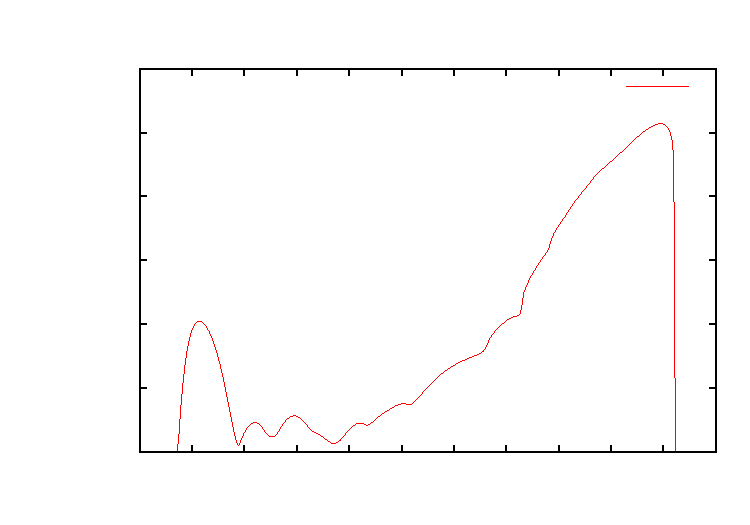
\includegraphics{diskecc1D}}%
    \gplfronttext
  \end{picture}%
\endgroup

	\end{center}
\caption{1D-Profil der Exzentrizitaet einer Disk nach einem Binary Orbit}
\end {figure}
\begin {figure}
	\begin{center}
		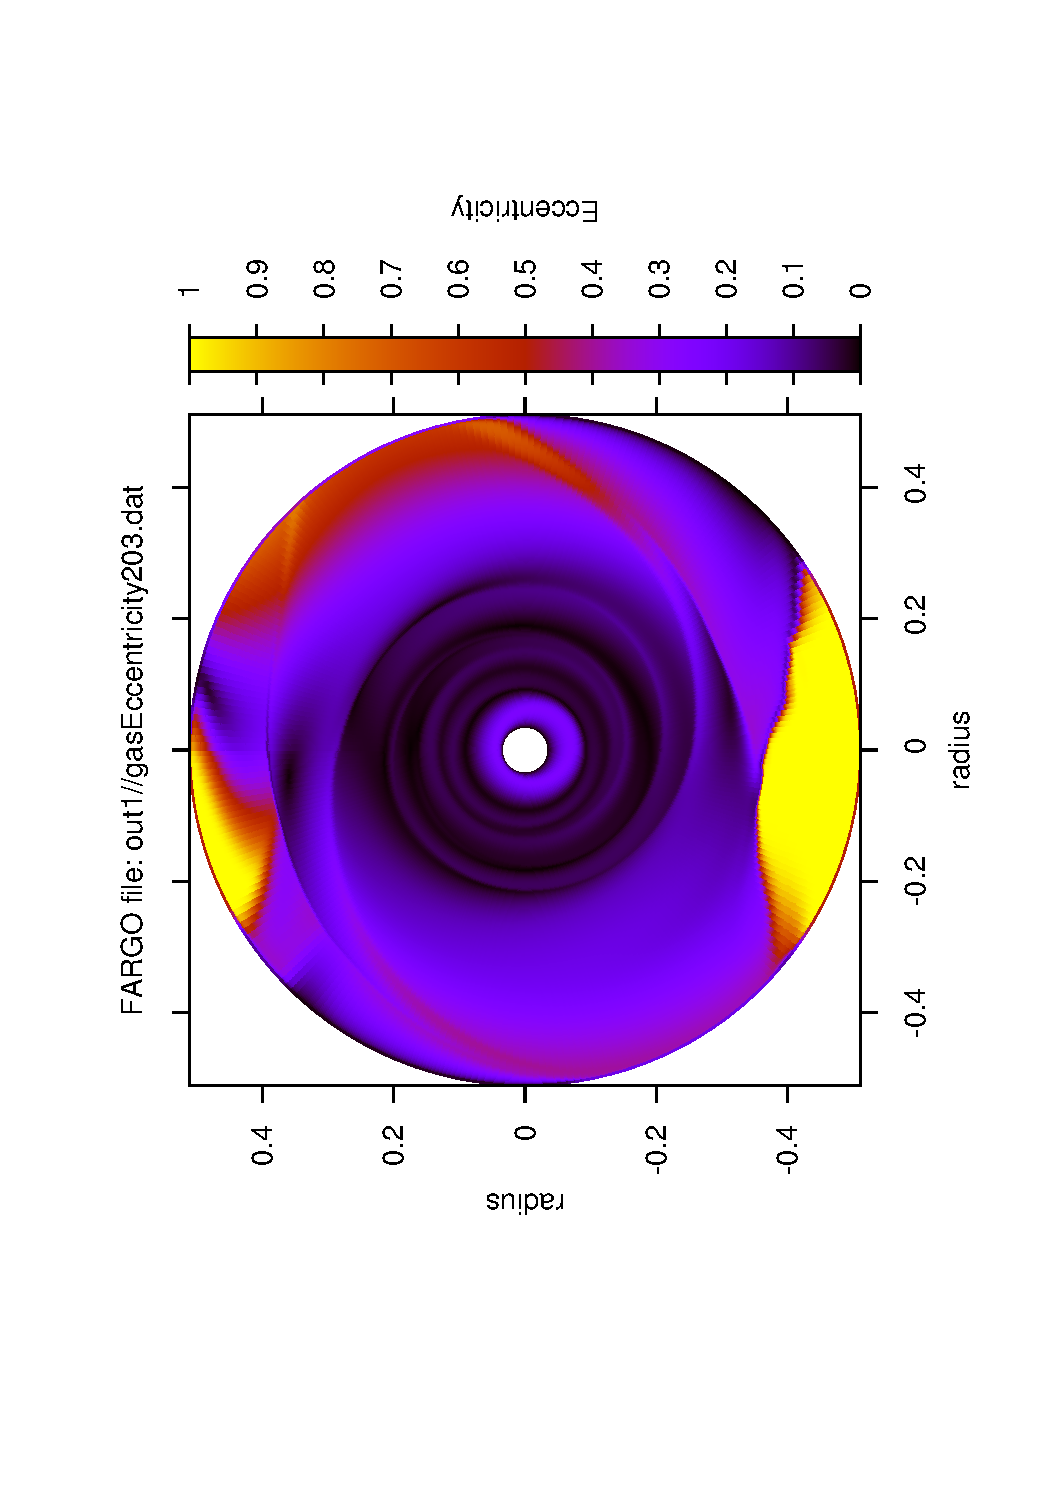
\includegraphics[scale=0.5,angle=270]{gasEccentricity203}
	\end{center}
\caption{2D-Profil der Exzentrizitaet einer Disk nach einem Binary Orbit}
\end {figure}

\subsection{CVNR}
Der FARGO-Code hat eine künstliche Viskosität in den Druck-Quelltermen. Um einen Vergleich mit RH2D und NIRVANA durchführen zu können, kann man jetzt die künstliche Viskosität in der Variable CVNR konfigurieren. Der Standardwert ist 1.41. Wenn man Rechnungen ohne kuenstliche Viskositaet durchfuehrt, kommt es in der Scheibe oft zu hohen Geschwindigkeiten einzelner Zellen. Dies kann zu einem Kollaps der Exzentrizitaet der Scheibe fuehren. Nach einer Weile erholt sich die Scheibe zwar wieder, doch macht das physikalisch einfach keinen Sinn:
\begin {figure}
	\begin{center}
		% GNUPLOT: LaTeX picture with Postscript
\begingroup
  \makeatletter
  \providecommand\color[2][]{%
    \GenericError{(gnuplot) \space\space\space\@spaces}{%
      Package color not loaded in conjunction with
      terminal option `colourtext'%
    }{See the gnuplot documentation for explanation.%
    }{Either use 'blacktext' in gnuplot or load the package
      color.sty in LaTeX.}%
    \renewcommand\color[2][]{}%
  }%
  \providecommand\includegraphics[2][]{%
    \GenericError{(gnuplot) \space\space\space\@spaces}{%
      Package graphicx or graphics not loaded%
    }{See the gnuplot documentation for explanation.%
    }{The gnuplot epslatex terminal needs graphicx.sty or graphics.sty.}%
    \renewcommand\includegraphics[2][]{}%
  }%
  \providecommand\rotatebox[2]{#2}%
  \@ifundefined{ifGPcolor}{%
    \newif\ifGPcolor
    \GPcolortrue
  }{}%
  \@ifundefined{ifGPblacktext}{%
    \newif\ifGPblacktext
    \GPblacktexttrue
  }{}%
  % define a \g@addto@macro without @ in the name:
  \let\gplgaddtomacro\g@addto@macro
  % define empty templates for all commands taking text:
  \gdef\gplbacktext{}%
  \gdef\gplfronttext{}%
  \makeatother
  \ifGPblacktext
    % no textcolor at all
    \def\colorrgb#1{}%
    \def\colorgray#1{}%
  \else
    % gray or color?
    \ifGPcolor
      \def\colorrgb#1{\color[rgb]{#1}}%
      \def\colorgray#1{\color[gray]{#1}}%
      \expandafter\def\csname LTw\endcsname{\color{white}}%
      \expandafter\def\csname LTb\endcsname{\color{black}}%
      \expandafter\def\csname LTa\endcsname{\color{black}}%
      \expandafter\def\csname LT0\endcsname{\color[rgb]{1,0,0}}%
      \expandafter\def\csname LT1\endcsname{\color[rgb]{0,1,0}}%
      \expandafter\def\csname LT2\endcsname{\color[rgb]{0,0,1}}%
      \expandafter\def\csname LT3\endcsname{\color[rgb]{1,0,1}}%
      \expandafter\def\csname LT4\endcsname{\color[rgb]{0,1,1}}%
      \expandafter\def\csname LT5\endcsname{\color[rgb]{1,1,0}}%
      \expandafter\def\csname LT6\endcsname{\color[rgb]{0,0,0}}%
      \expandafter\def\csname LT7\endcsname{\color[rgb]{1,0.3,0}}%
      \expandafter\def\csname LT8\endcsname{\color[rgb]{0.5,0.5,0.5}}%
    \else
      % gray
      \def\colorrgb#1{\color{black}}%
      \def\colorgray#1{\color[gray]{#1}}%
      \expandafter\def\csname LTw\endcsname{\color{white}}%
      \expandafter\def\csname LTb\endcsname{\color{black}}%
      \expandafter\def\csname LTa\endcsname{\color{black}}%
      \expandafter\def\csname LT0\endcsname{\color{black}}%
      \expandafter\def\csname LT1\endcsname{\color{black}}%
      \expandafter\def\csname LT2\endcsname{\color{black}}%
      \expandafter\def\csname LT3\endcsname{\color{black}}%
      \expandafter\def\csname LT4\endcsname{\color{black}}%
      \expandafter\def\csname LT5\endcsname{\color{black}}%
      \expandafter\def\csname LT6\endcsname{\color{black}}%
      \expandafter\def\csname LT7\endcsname{\color{black}}%
      \expandafter\def\csname LT8\endcsname{\color{black}}%
    \fi
  \fi
  \setlength{\unitlength}{0.0500bp}%
  \begin{picture}(7200.00,5040.00)%
    \gplgaddtomacro\gplbacktext{%
      \csname LTb\endcsname%
      \put(1210,704){\makebox(0,0)[r]{\strut{} 0}}%
      \csname LTb\endcsname%
      \put(1210,1439){\makebox(0,0)[r]{\strut{} 0.2}}%
      \csname LTb\endcsname%
      \put(1210,2174){\makebox(0,0)[r]{\strut{} 0.4}}%
      \csname LTb\endcsname%
      \put(1210,2910){\makebox(0,0)[r]{\strut{} 0.6}}%
      \csname LTb\endcsname%
      \put(1210,3645){\makebox(0,0)[r]{\strut{} 0.8}}%
      \csname LTb\endcsname%
      \put(1210,4380){\makebox(0,0)[r]{\strut{} 1}}%
      \csname LTb\endcsname%
      \put(1342,484){\makebox(0,0){\strut{} 0}}%
      \csname LTb\endcsname%
      \put(2033,484){\makebox(0,0){\strut{} 20}}%
      \csname LTb\endcsname%
      \put(2724,484){\makebox(0,0){\strut{} 40}}%
      \csname LTb\endcsname%
      \put(3415,484){\makebox(0,0){\strut{} 60}}%
      \csname LTb\endcsname%
      \put(4106,484){\makebox(0,0){\strut{} 80}}%
      \csname LTb\endcsname%
      \put(4797,484){\makebox(0,0){\strut{} 100}}%
      \csname LTb\endcsname%
      \put(5488,484){\makebox(0,0){\strut{} 120}}%
      \csname LTb\endcsname%
      \put(6179,484){\makebox(0,0){\strut{} 140}}%
      \csname LTb\endcsname%
      \put(6870,484){\makebox(0,0){\strut{} 160}}%
      \put(440,2542){\rotatebox{90}{\makebox(0,0){\strut{}Eccentricity}}}%
      \put(4106,154){\makebox(0,0){\strut{}Time [Years]}}%
      \put(4106,4710){\makebox(0,0){\strut{}h = 0.04}}%
    }%
    \gplgaddtomacro\gplfronttext{%
      \csname LTb\endcsname%
      \put(5883,4207){\makebox(0,0)[r]{\strut{}q=0.1}}%
      \csname LTb\endcsname%
      \put(5883,3987){\makebox(0,0)[r]{\strut{}q=0.2}}%
      \csname LTb\endcsname%
      \put(5883,3767){\makebox(0,0)[r]{\strut{}q=0.3}}%
      \csname LTb\endcsname%
      \put(5883,3547){\makebox(0,0)[r]{\strut{}q=0.4}}%
      \csname LTb\endcsname%
      \put(5883,3327){\makebox(0,0)[r]{\strut{}q=0.5}}%
      \csname LTb\endcsname%F
      \put(5883,3107){\makebox(0,0)[r]{\strut{}q=0.6}}%
      \csname LTb\endcsname%
      \put(5883,2887){\makebox(0,0)[r]{\strut{}q=0.7}}%
      \csname LTb\endcsname%
      \put(5883,2667){\makebox(0,0)[r]{\strut{}q=0.8}}%
      \csname LTb\endcsname%
      \put(5883,2447){\makebox(0,0)[r]{\strut{}q=0.9}}%
      \csname LTb\endcsname%
      \put(5883,2227){\makebox(0,0)[r]{\strut{}q=1.0}}%
    }%
    \gplbacktext
    \put(0,0){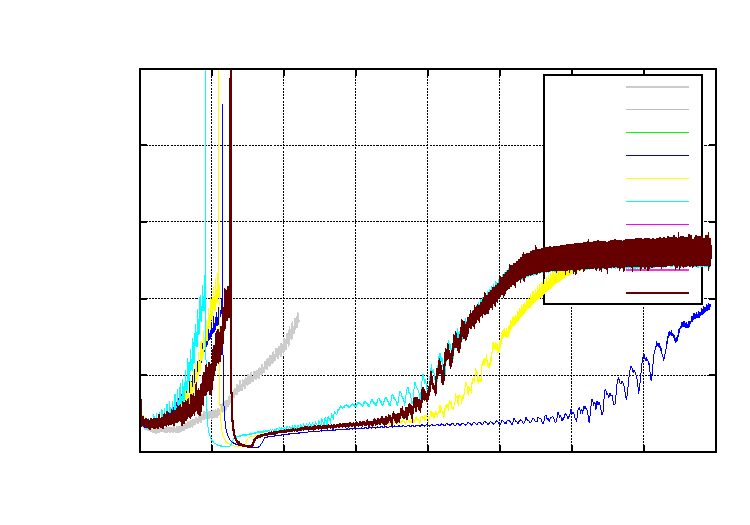
\includegraphics{CVNRCollapse}}%
    \gplfronttext
  \end{picture}%
\endgroup

	\end{center}
\caption{Ohne kuenstliche Viskositaet werden Zellen am Rand der Disk sehr schnell und bringen die Disk zum kollabieren.}
\end {figure}


Wenn man dieselbe Rechnung mit CVNR = 1.41 berechnet, hat man anfangs dieselbe Steigung und den Selben Endwert, aber nicht den starken Abfall dazwischen.
\subsection{Boundary-Conditions}
FARGO hat folgende Randbedingungen implementiert:
\begin{itemize}
\item Open:
Bei offenen Randbedingungen geht sehr viel Masse verloren:
\begin {figure}
	\begin{center}
		% GNUPLOT: LaTeX picture with Postscript
\begingroup
  \makeatletter
  \providecommand\color[2][]{%
    \GenericError{(gnuplot) \space\space\space\@spaces}{%
      Package color not loaded in conjunction with
      terminal option `colourtext'%
    }{See the gnuplot documentation for explanation.%
    }{Either use 'blacktext' in gnuplot or load the package
      color.sty in LaTeX.}%
    \renewcommand\color[2][]{}%
  }%
  \providecommand\includegraphics[2][]{%
    \GenericError{(gnuplot) \space\space\space\@spaces}{%
      Package graphicx or graphics not loaded%
    }{See the gnuplot documentation for explanation.%
    }{The gnuplot epslatex terminal needs graphicx.sty or graphics.sty.}%
    \renewcommand\includegraphics[2][]{}%
  }%
  \providecommand\rotatebox[2]{#2}%
  \@ifundefined{ifGPcolor}{%
    \newif\ifGPcolor
    \GPcolortrue
  }{}%
  \@ifundefined{ifGPblacktext}{%
    \newif\ifGPblacktext
    \GPblacktexttrue
  }{}%
  % define a \g@addto@macro without @ in the name:
  \let\gplgaddtomacro\g@addto@macro
  % define empty templates for all commands taking text:
  \gdef\gplbacktext{}%
  \gdef\gplfronttext{}%
  \makeatother
  \ifGPblacktext
    % no textcolor at all
    \def\colorrgb#1{}%
    \def\colorgray#1{}%
  \else
    % gray or color?
    \ifGPcolor
      \def\colorrgb#1{\color[rgb]{#1}}%
      \def\colorgray#1{\color[gray]{#1}}%
      \expandafter\def\csname LTw\endcsname{\color{white}}%
      \expandafter\def\csname LTb\endcsname{\color{black}}%
      \expandafter\def\csname LTa\endcsname{\color{black}}%
      \expandafter\def\csname LT0\endcsname{\color[rgb]{1,0,0}}%
      \expandafter\def\csname LT1\endcsname{\color[rgb]{0,1,0}}%
      \expandafter\def\csname LT2\endcsname{\color[rgb]{0,0,1}}%
      \expandafter\def\csname LT3\endcsname{\color[rgb]{1,0,1}}%
      \expandafter\def\csname LT4\endcsname{\color[rgb]{0,1,1}}%
      \expandafter\def\csname LT5\endcsname{\color[rgb]{1,1,0}}%
      \expandafter\def\csname LT6\endcsname{\color[rgb]{0,0,0}}%
      \expandafter\def\csname LT7\endcsname{\color[rgb]{1,0.3,0}}%
      \expandafter\def\csname LT8\endcsname{\color[rgb]{0.5,0.5,0.5}}%
    \else
      % gray
      \def\colorrgb#1{\color{black}}%
      \def\colorgray#1{\color[gray]{#1}}%
      \expandafter\def\csname LTw\endcsname{\color{white}}%
      \expandafter\def\csname LTb\endcsname{\color{black}}%
      \expandafter\def\csname LTa\endcsname{\color{black}}%
      \expandafter\def\csname LT0\endcsname{\color{black}}%
      \expandafter\def\csname LT1\endcsname{\color{black}}%
      \expandafter\def\csname LT2\endcsname{\color{black}}%
      \expandafter\def\csname LT3\endcsname{\color{black}}%
      \expandafter\def\csname LT4\endcsname{\color{black}}%
      \expandafter\def\csname LT5\endcsname{\color{black}}%
      \expandafter\def\csname LT6\endcsname{\color{black}}%
      \expandafter\def\csname LT7\endcsname{\color{black}}%
      \expandafter\def\csname LT8\endcsname{\color{black}}%
    \fi
  \fi
  \setlength{\unitlength}{0.0500bp}%
  \begin{picture}(7200.00,5040.00)%
    \gplgaddtomacro\gplbacktext{%
      \csname LTb\endcsname%
      \put(1738,704){\makebox(0,0)[r]{\strut{} 0.00075}}%
      \put(1738,1229){\makebox(0,0)[r]{\strut{} 0.0008}}%
      \put(1738,1754){\makebox(0,0)[r]{\strut{} 0.00085}}%
      \put(1738,2279){\makebox(0,0)[r]{\strut{} 0.0009}}%
      \put(1738,2805){\makebox(0,0)[r]{\strut{} 0.00095}}%
      \put(1738,3330){\makebox(0,0)[r]{\strut{} 0.001}}%
      \put(1738,3855){\makebox(0,0)[r]{\strut{} 0.00105}}%
      \put(1738,4380){\makebox(0,0)[r]{\strut{} 0.0011}}%
      \put(1870,484){\makebox(0,0){\strut{} 0}}%
      \put(2703,484){\makebox(0,0){\strut{} 1000}}%
      \put(3537,484){\makebox(0,0){\strut{} 2000}}%
      \put(4370,484){\makebox(0,0){\strut{} 3000}}%
      \put(5203,484){\makebox(0,0){\strut{} 4000}}%
      \put(6037,484){\makebox(0,0){\strut{} 5000}}%
      \put(6870,484){\makebox(0,0){\strut{} 6000}}%
      \put(440,2542){\rotatebox{90}{\makebox(0,0){\strut{}Mass [$M_{astrosun}$]}}}%
      \put(4370,154){\makebox(0,0){\strut{}Time [Years]}}%
      \put(4370,4710){\makebox(0,0){\strut{}Disk Mass}}%
    }%
    \gplgaddtomacro\gplfronttext{%
      \csname LTb\endcsname%
      \put(5883,4207){\makebox(0,0)[r]{\strut{}Mass}}%
    }%
    \gplbacktext
    \put(0,0){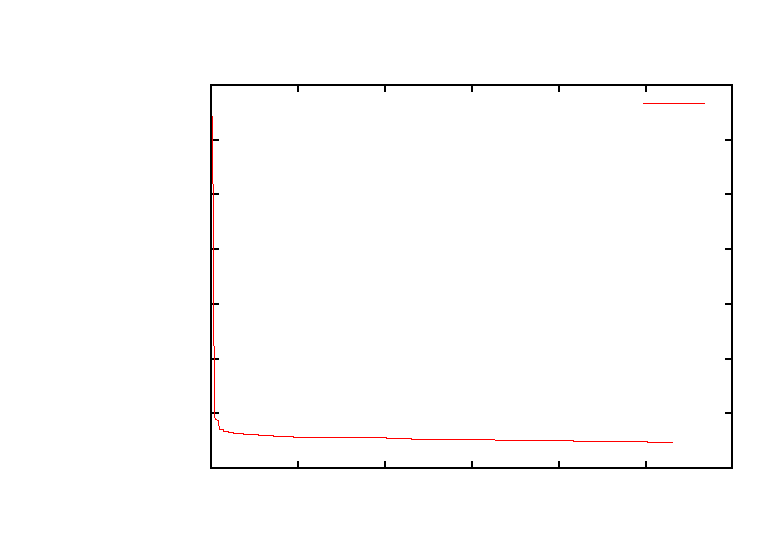
\includegraphics{diskmass}}%
    \gplfronttext
  \end{picture}%
\endgroup

	\end{center}
\caption{Masseverlust der Disk: Nach dem ersten Binaersternorbit geht der Grossteil der Masse verloren.}
\end {figure}
\item Reflecting
\item Non-Reflecting, Evanescent haben wir nicht verwendet.
\end{itemize}
\section{Potential-Smoothing}
Wenn sich ein Planet in der Akkretionsscheibe befindet, so wird sein Potential mit $\frac{1}{(r+\epsilon)^2}$ geglaettet.
Wenn wir eine Akkretionsscheibe in einem Binärsternsystem betrachten, müssen wir, um sinnvolle Ergebnisse zu erhalten, den Binärstern anders betrachten als einen Planeten: Die Entfernung eines Planeten ist viel geringer. Bei Binaersternen macht also Potential-Smoothing keinen Sinn. Hier hilft man sich, indem man das Thicknesssmoothing auf z.B. $\epsilon=10^-{9}$ setzt und somit die Abfrage fuer das Roche-Smoothing umgeht.
\section{Modellierung exzentrischer Binaersternsysteme}
Die exzentrische Bahn des Binaersterns stoert und veraendert die Disk signifikant! Durch hohe Exzentrizitaeten fliegt der Stern im Periastron sehr nah an der Disk vorbei und setzt sie somit bei jedem Binary Orbit grossen Kraeften aus. Dies fuehrt offensichtlich bei jedem Binary Orbit zu einer starken Aenderung der Exzentrizitaet. Doch was passiert, wenn man sich eine groessere Zeitspanne und somit mehrere Binary Orbits ansieht? Das wollen wir im Folgenden herausfinden.
\subsection{$\gamma$ Cep}
Physikalische Parameter:


\begin{tabular}{|c|c|c|c|c|c|c|}
\hline$M_1$ & $M_2$ & a & e & $M_p$ & $a_p$ & $e_p$\\\hline
1.59 & 0.378 & 18.5 & 0.36 & 1.70 & 2.13 & 0.20\\\hline
\end{tabular}


Diese physikalischen Parameter kann man nicht immer direkt in FARGO uebertragen: FARGO verwendet als Masse fuer den Primaerstern immer 1, also muss man die Masse des Binaersterns entsprechend skalieren: $M_1 = 1.0 ; M_2 = 0.2378$. Wir beruecksichtigen hier keine Wechselwirkung des Binaersterns mit der Scheibe, d.h. der Binaerstern ist auf seiner festen Bahn. Mittels der config File fuer die Planeten kann man auch Wechselwirkung mit der Disk und anderen Planeten einschalten, das ist aber noch nicht getestet worden. Genau so mit Vorsicht muss man die Code-Zeit betrachten. Nur mit dem richtigen Umrechenfaktor ergibt sich die korrekte Zeit fuer die Orbits. Bei einem Orbit von 1 $\unit{AU}$ ist der Faktor z.B. $0.126212$
\begin {figure}
	\begin{center}
		% GNUPLOT: LaTeX picture with Postscript
\begingroup
  \makeatletter
  \providecommand\color[2][]{%
    \GenericError{(gnuplot) \space\space\space\@spaces}{%
      Package color not loaded in conjunction with
      terminal option `colourtext'%
    }{See the gnuplot documentation for explanation.%
    }{Either use 'blacktext' in gnuplot or load the package
      color.sty in LaTeX.}%
    \renewcommand\color[2][]{}%
  }%
  \providecommand\includegraphics[2][]{%
    \GenericError{(gnuplot) \space\space\space\@spaces}{%
      Package graphicx or graphics not loaded%
    }{See the gnuplot documentation for explanation.%
    }{The gnuplot epslatex terminal needs graphicx.sty or graphics.sty.}%
    \renewcommand\includegraphics[2][]{}%
  }%
  \providecommand\rotatebox[2]{#2}%
  \@ifundefined{ifGPcolor}{%
    \newif\ifGPcolor
    \GPcolortrue
  }{}%
  \@ifundefined{ifGPblacktext}{%
    \newif\ifGPblacktext
    \GPblacktexttrue
  }{}%
  % define a \g@addto@macro without @ in the name:
  \let\gplgaddtomacro\g@addto@macro
  % define empty templates for all commands taking text:
  \gdef\gplbacktext{}%
  \gdef\gplfronttext{}%
  \makeatother
  \ifGPblacktext
    % no textcolor at all
    \def\colorrgb#1{}%
    \def\colorgray#1{}%
  \else
    % gray or color?
    \ifGPcolor
      \def\colorrgb#1{\color[rgb]{#1}}%
      \def\colorgray#1{\color[gray]{#1}}%
      \expandafter\def\csname LTw\endcsname{\color{white}}%
      \expandafter\def\csname LTb\endcsname{\color{black}}%
      \expandafter\def\csname LTa\endcsname{\color{black}}%
      \expandafter\def\csname LT0\endcsname{\color[rgb]{1,0,0}}%
      \expandafter\def\csname LT1\endcsname{\color[rgb]{0,1,0}}%
      \expandafter\def\csname LT2\endcsname{\color[rgb]{0,0,1}}%
      \expandafter\def\csname LT3\endcsname{\color[rgb]{1,0,1}}%
      \expandafter\def\csname LT4\endcsname{\color[rgb]{0,1,1}}%
      \expandafter\def\csname LT5\endcsname{\color[rgb]{1,1,0}}%
      \expandafter\def\csname LT6\endcsname{\color[rgb]{0,0,0}}%
      \expandafter\def\csname LT7\endcsname{\color[rgb]{1,0.3,0}}%
      \expandafter\def\csname LT8\endcsname{\color[rgb]{0.5,0.5,0.5}}%
    \else
      % gray
      \def\colorrgb#1{\color{black}}%
      \def\colorgray#1{\color[gray]{#1}}%
      \expandafter\def\csname LTw\endcsname{\color{white}}%
      \expandafter\def\csname LTb\endcsname{\color{black}}%
      \expandafter\def\csname LTa\endcsname{\color{black}}%
      \expandafter\def\csname LT0\endcsname{\color{black}}%
      \expandafter\def\csname LT1\endcsname{\color{black}}%
      \expandafter\def\csname LT2\endcsname{\color{black}}%
      \expandafter\def\csname LT3\endcsname{\color{black}}%
      \expandafter\def\csname LT4\endcsname{\color{black}}%
      \expandafter\def\csname LT5\endcsname{\color{black}}%
      \expandafter\def\csname LT6\endcsname{\color{black}}%
      \expandafter\def\csname LT7\endcsname{\color{black}}%
      \expandafter\def\csname LT8\endcsname{\color{black}}%
    \fi
  \fi
  \setlength{\unitlength}{0.0500bp}%
  \begin{picture}(7200.00,5040.00)%
    \gplgaddtomacro\gplbacktext{%
      \csname LTb\endcsname%
      \put(1872,1153){\makebox(0,0)[r]{\strut{}-20}}%
      \put(1872,1947){\makebox(0,0)[r]{\strut{}-10}}%
      \put(1872,2740){\makebox(0,0)[r]{\strut{} 0}}%
      \put(1872,3533){\makebox(0,0)[r]{\strut{} 10}}%
      \put(1872,4327){\makebox(0,0)[r]{\strut{} 20}}%
      \put(2255,484){\makebox(0,0){\strut{}-10}}%
      \put(2791,484){\makebox(0,0){\strut{}-5}}%
      \put(3326,484){\makebox(0,0){\strut{} 0}}%
      \put(3862,484){\makebox(0,0){\strut{} 5}}%
      \put(4398,484){\makebox(0,0){\strut{} 10}}%
      \put(4934,484){\makebox(0,0){\strut{} 15}}%
      \put(5469,484){\makebox(0,0){\strut{} 20}}%
      \put(6005,484){\makebox(0,0){\strut{} 25}}%
      \put(1234,2740){\rotatebox{90}{\makebox(0,0){\strut{}y}}}%
      \put(4040,154){\makebox(0,0){\strut{}x}}%
    }%
    \gplgaddtomacro\gplfronttext{%
      \csname LTb\endcsname%
      \put(5089,4603){\makebox(0,0)[r]{\strut{}Primary Star}}%
      \csname LTb\endcsname%
      \put(5089,4383){\makebox(0,0)[r]{\strut{}Bahn}}%
      \csname LTb\endcsname%
      \put(5089,4163){\makebox(0,0)[r]{\strut{}Binary Star}}%
    }%
    \gplbacktext
    \put(0,0){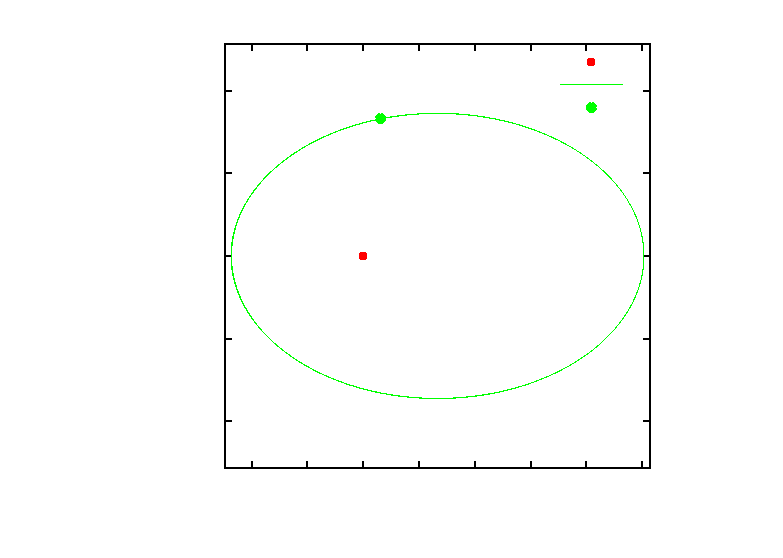
\includegraphics{binstar}}%
    \gplfronttext
  \end{picture}%
\endgroup

	\end{center}
\caption{Der Binaerstern umrundet den Primaerstern auf seiner festen Umlaufbahn. Um die Fehler der Bewegung zu ueberpruefen, wird die zuvor angegebene Exzentrizitaet anhand der Bewegung berechnet.}
\end {figure}

Um erste Tests und einen Vergleich mit Kleys RH2D durchzufuehren, wurde das Setup von $\gamma$ Cep verwendet. Es werden die Dichteprofile, Exzentrizitaetsprofile nach einigen Binaerorbits untersucht.
\begin {figure}
	\begin{center}
		% GNUPLOT: LaTeX picture with Postscript
\begingroup
  \makeatletter
  \providecommand\color[2][]{%
    \GenericError{(gnuplot) \space\space\space\@spaces}{%
      Package color not loaded in conjunction with
      terminal option `colourtext'%
    }{See the gnuplot documentation for explanation.%
    }{Either use 'blacktext' in gnuplot or load the package
      color.sty in LaTeX.}%
    \renewcommand\color[2][]{}%
  }%
  \providecommand\includegraphics[2][]{%
    \GenericError{(gnuplot) \space\space\space\@spaces}{%
      Package graphicx or graphics not loaded%
    }{See the gnuplot documentation for explanation.%
    }{The gnuplot epslatex terminal needs graphicx.sty or graphics.sty.}%
    \renewcommand\includegraphics[2][]{}%
  }%
  \providecommand\rotatebox[2]{#2}%
  \@ifundefined{ifGPcolor}{%
    \newif\ifGPcolor
    \GPcolortrue
  }{}%
  \@ifundefined{ifGPblacktext}{%
    \newif\ifGPblacktext
    \GPblacktexttrue
  }{}%
  % define a \g@addto@macro without @ in the name:
  \let\gplgaddtomacro\g@addto@macro
  % define empty templates for all commands taking text:
  \gdef\gplbacktext{}%
  \gdef\gplfronttext{}%
  \makeatother
  \ifGPblacktext
    % no textcolor at all
    \def\colorrgb#1{}%
    \def\colorgray#1{}%
  \else
    % gray or color?
    \ifGPcolor
      \def\colorrgb#1{\color[rgb]{#1}}%
      \def\colorgray#1{\color[gray]{#1}}%
      \expandafter\def\csname LTw\endcsname{\color{white}}%
      \expandafter\def\csname LTb\endcsname{\color{black}}%
      \expandafter\def\csname LTa\endcsname{\color{black}}%
      \expandafter\def\csname LT0\endcsname{\color[rgb]{1,0,0}}%
      \expandafter\def\csname LT1\endcsname{\color[rgb]{0,1,0}}%
      \expandafter\def\csname LT2\endcsname{\color[rgb]{0,0,1}}%
      \expandafter\def\csname LT3\endcsname{\color[rgb]{1,0,1}}%
      \expandafter\def\csname LT4\endcsname{\color[rgb]{0,1,1}}%
      \expandafter\def\csname LT5\endcsname{\color[rgb]{1,1,0}}%
      \expandafter\def\csname LT6\endcsname{\color[rgb]{0,0,0}}%
      \expandafter\def\csname LT7\endcsname{\color[rgb]{1,0.3,0}}%
      \expandafter\def\csname LT8\endcsname{\color[rgb]{0.5,0.5,0.5}}%
    \else
      % gray
      \def\colorrgb#1{\color{black}}%
      \def\colorgray#1{\color[gray]{#1}}%
      \expandafter\def\csname LTw\endcsname{\color{white}}%
      \expandafter\def\csname LTb\endcsname{\color{black}}%
      \expandafter\def\csname LTa\endcsname{\color{black}}%
      \expandafter\def\csname LT0\endcsname{\color{black}}%
      \expandafter\def\csname LT1\endcsname{\color{black}}%
      \expandafter\def\csname LT2\endcsname{\color{black}}%
      \expandafter\def\csname LT3\endcsname{\color{black}}%
      \expandafter\def\csname LT4\endcsname{\color{black}}%
      \expandafter\def\csname LT5\endcsname{\color{black}}%
      \expandafter\def\csname LT6\endcsname{\color{black}}%
      \expandafter\def\csname LT7\endcsname{\color{black}}%
      \expandafter\def\csname LT8\endcsname{\color{black}}%
    \fi
  \fi
  \setlength{\unitlength}{0.0500bp}%
  \begin{picture}(7200.00,5040.00)%
    \gplgaddtomacro\gplbacktext{%
      \csname LTb\endcsname%
      \put(1210,704){\makebox(0,0)[r]{\strut{} 0}}%
      \put(1210,1229){\makebox(0,0)[r]{\strut{} 100}}%
      \put(1210,1754){\makebox(0,0)[r]{\strut{} 200}}%
      \put(1210,2279){\makebox(0,0)[r]{\strut{} 300}}%
      \put(1210,2805){\makebox(0,0)[r]{\strut{} 400}}%
      \put(1210,3330){\makebox(0,0)[r]{\strut{} 500}}%
      \put(1210,3855){\makebox(0,0)[r]{\strut{} 600}}%
      \put(1210,4380){\makebox(0,0)[r]{\strut{} 700}}%
      \put(1711,484){\makebox(0,0){\strut{} 1}}%
      \put(2448,484){\makebox(0,0){\strut{} 2}}%
      \put(3185,484){\makebox(0,0){\strut{} 3}}%
      \put(3922,484){\makebox(0,0){\strut{} 4}}%
      \put(4659,484){\makebox(0,0){\strut{} 5}}%
      \put(5396,484){\makebox(0,0){\strut{} 6}}%
      \put(6133,484){\makebox(0,0){\strut{} 7}}%
      \put(6870,484){\makebox(0,0){\strut{} 8}}%
      \put(440,2542){\rotatebox{90}{\makebox(0,0){\strut{}Sigma}}}%
      \put(4106,154){\makebox(0,0){\strut{}r [AU]}}%
      \put(4106,4710){\makebox(0,0){\strut{}Density Profile in Binary Orbits}}%
    }%
    \gplgaddtomacro\gplfronttext{%
      \csname LTb\endcsname%
      \put(5883,4207){\makebox(0,0)[r]{\strut{}0 $Orb_{Bin}$}}%
      \csname LTb\endcsname%
      \put(5883,3987){\makebox(0,0)[r]{\strut{}5 $Orb_{Bin}$}}%
      \csname LTb\endcsname%
      \put(5883,3767){\makebox(0,0)[r]{\strut{}10 $Orb_{Bin}$}}%
      \csname LTb\endcsname%
      \put(5883,3547){\makebox(0,0)[r]{\strut{}15 $Orb_{Bin}$}}%
      \csname LTb\endcsname%
      \put(5883,3327){\makebox(0,0)[r]{\strut{}20 $Orb_{Bin}$}}%
      \csname LTb\endcsname%
      \put(5883,3107){\makebox(0,0)[r]{\strut{}30 $Orb_{Bin}$}}%
      \csname LTb\endcsname%
      \put(5883,2887){\makebox(0,0)[r]{\strut{}40 $Orb_{Bin}$}}%
      \csname LTb\endcsname%
      \put(5883,2667){\makebox(0,0)[r]{\strut{}60 $Orb_{Bin}$}}%
    }%
    \gplbacktext
    \put(0,0){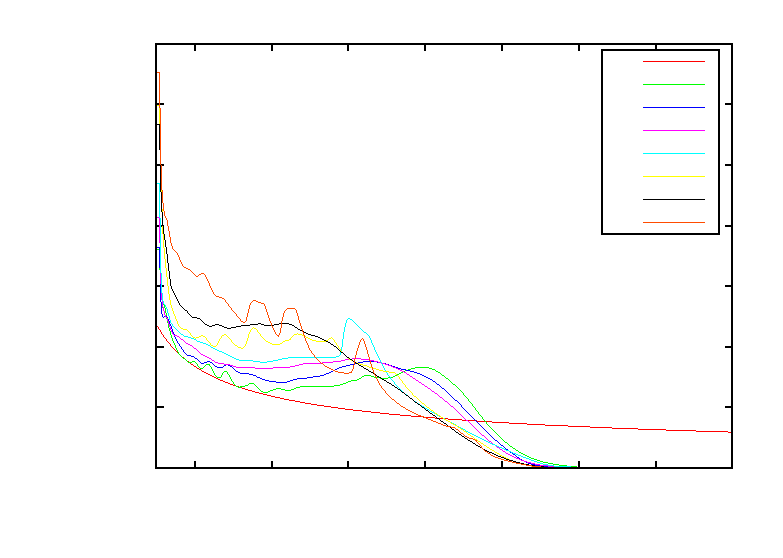
\includegraphics{densityprofile}}%
    \gplfronttext
  \end{picture}%
\endgroup

	\end{center}
\caption{Die Entwicklung des Dichteprofils ist analog zu Kley/Nelson}
TODO: exentrizitaetsprofil
\end {figure}

Die zeitliche Entwicklung der Exzentrizitaet der Scheibe von $\gamma$ Cep geht auch in Einklang mit Kleys Ergebnissen.

\begin {figure}
	\begin{center}
		% GNUPLOT: LaTeX picture with Postscript
\begingroup
  \makeatletter
  \providecommand\color[2][]{%
    \GenericError{(gnuplot) \space\space\space\@spaces}{%
      Package color not loaded in conjunction with
      terminal option `colourtext'%
    }{See the gnuplot documentation for explanation.%
    }{Either use 'blacktext' in gnuplot or load the package
      color.sty in LaTeX.}%
    \renewcommand\color[2][]{}%
  }%
  \providecommand\includegraphics[2][]{%
    \GenericError{(gnuplot) \space\space\space\@spaces}{%
      Package graphicx or graphics not loaded%
    }{See the gnuplot documentation for explanation.%
    }{The gnuplot epslatex terminal needs graphicx.sty or graphics.sty.}%
    \renewcommand\includegraphics[2][]{}%
  }%
  \providecommand\rotatebox[2]{#2}%
  \@ifundefined{ifGPcolor}{%
    \newif\ifGPcolor
    \GPcolortrue
  }{}%
  \@ifundefined{ifGPblacktext}{%
    \newif\ifGPblacktext
    \GPblacktexttrue
  }{}%
  % define a \g@addto@macro without @ in the name:
  \let\gplgaddtomacro\g@addto@macro
  % define empty templates for all commands taking text:
  \gdef\gplbacktext{}%
  \gdef\gplfronttext{}%
  \makeatother
  \ifGPblacktext
    % no textcolor at all
    \def\colorrgb#1{}%
    \def\colorgray#1{}%
  \else
    % gray or color?
    \ifGPcolor
      \def\colorrgb#1{\color[rgb]{#1}}%
      \def\colorgray#1{\color[gray]{#1}}%
      \expandafter\def\csname LTw\endcsname{\color{white}}%
      \expandafter\def\csname LTb\endcsname{\color{black}}%
      \expandafter\def\csname LTa\endcsname{\color{black}}%
      \expandafter\def\csname LT0\endcsname{\color[rgb]{1,0,0}}%
      \expandafter\def\csname LT1\endcsname{\color[rgb]{0,1,0}}%
      \expandafter\def\csname LT2\endcsname{\color[rgb]{0,0,1}}%
      \expandafter\def\csname LT3\endcsname{\color[rgb]{1,0,1}}%
      \expandafter\def\csname LT4\endcsname{\color[rgb]{0,1,1}}%
      \expandafter\def\csname LT5\endcsname{\color[rgb]{1,1,0}}%
      \expandafter\def\csname LT6\endcsname{\color[rgb]{0,0,0}}%
      \expandafter\def\csname LT7\endcsname{\color[rgb]{1,0.3,0}}%
      \expandafter\def\csname LT8\endcsname{\color[rgb]{0.5,0.5,0.5}}%
    \else
      % gray
      \def\colorrgb#1{\color{black}}%
      \def\colorgray#1{\color[gray]{#1}}%
      \expandafter\def\csname LTw\endcsname{\color{white}}%
      \expandafter\def\csname LTb\endcsname{\color{black}}%
      \expandafter\def\csname LTa\endcsname{\color{black}}%
      \expandafter\def\csname LT0\endcsname{\color{black}}%
      \expandafter\def\csname LT1\endcsname{\color{black}}%
      \expandafter\def\csname LT2\endcsname{\color{black}}%
      \expandafter\def\csname LT3\endcsname{\color{black}}%
      \expandafter\def\csname LT4\endcsname{\color{black}}%
      \expandafter\def\csname LT5\endcsname{\color{black}}%
      \expandafter\def\csname LT6\endcsname{\color{black}}%
      \expandafter\def\csname LT7\endcsname{\color{black}}%
      \expandafter\def\csname LT8\endcsname{\color{black}}%
    \fi
  \fi
  \setlength{\unitlength}{0.0500bp}%
  \begin{picture}(7200.00,5040.00)%
    \gplgaddtomacro\gplbacktext{%
      \csname LTb\endcsname%
      \put(1342,704){\makebox(0,0)[r]{\strut{} 0}}%
      \put(1342,1439){\makebox(0,0)[r]{\strut{} 0.05}}%
      \put(1342,2174){\makebox(0,0)[r]{\strut{} 0.1}}%
      \put(1342,2910){\makebox(0,0)[r]{\strut{} 0.15}}%
      \put(1342,3645){\makebox(0,0)[r]{\strut{} 0.2}}%
      \put(1342,4380){\makebox(0,0)[r]{\strut{} 0.25}}%
      \put(1474,484){\makebox(0,0){\strut{} 0}}%
      \put(2553,484){\makebox(0,0){\strut{} 20}}%
      \put(3632,484){\makebox(0,0){\strut{} 40}}%
      \put(4712,484){\makebox(0,0){\strut{} 60}}%
      \put(5791,484){\makebox(0,0){\strut{} 80}}%
      \put(6870,484){\makebox(0,0){\strut{} 100}}%
      \put(440,2542){\rotatebox{90}{\makebox(0,0){\strut{}Eccentricity}}}%
      \put(4172,154){\makebox(0,0){\strut{}Time [$Orb_{Bin}$]}}%
      \put(4172,4710){\makebox(0,0){\strut{}FARGO vs RH2D}}%
    }%
    \gplgaddtomacro\gplfronttext{%
      \csname LTb\endcsname%
      \put(5883,4207){\makebox(0,0)[r]{\strut{}FARGO}}%
      \csname LTb\endcsname%
      \put(5883,3987){\makebox(0,0)[r]{\strut{}RH2D}}%
    }%
    \gplbacktext
    \put(0,0){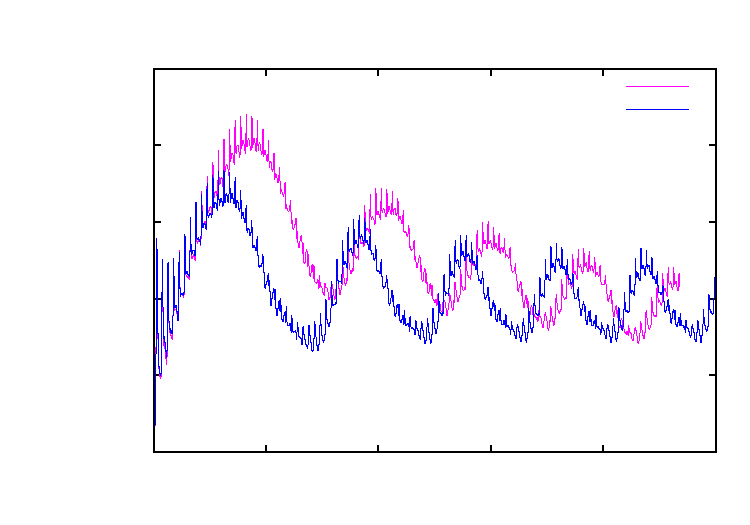
\includegraphics{diskecccomparefargorh2d}}%
    \gplfronttext
  \end{picture}%
\endgroup

	\end{center}
\caption{Anfangs schwingt FARGO etwas staerker, der spaetere Verlauf ist aber identisch}
\end {figure}

\clearpage
\section{Marzari Paper}
Setup:

\begin{tabular}{|c|c|c|c|c|c|c|}
\hline$M_1$ & $M_2$ & a & e & Rmin & Rmax & $e_p$\\\hline
1.0 & 0.4 & 30 & 0.4 & 0.5 & 15 & 0.20\\\hline
\end{tabular}


256x512 logarithmic Grid, Nonreflecting/Nonreflecting Randbedingungen
\section{Vergleich FARGO, Nirvana und RH2D}
\begin {figure}
	\begin{center}
		% GNUPLOT: LaTeX picture with Postscript
\begingroup
  \makeatletter
  \providecommand\color[2][]{%
    \GenericError{(gnuplot) \space\space\space\@spaces}{%
      Package color not loaded in conjunction with
      terminal option `colourtext'%
    }{See the gnuplot documentation for explanation.%
    }{Either use 'blacktext' in gnuplot or load the package
      color.sty in LaTeX.}%
    \renewcommand\color[2][]{}%
  }%
  \providecommand\includegraphics[2][]{%
    \GenericError{(gnuplot) \space\space\space\@spaces}{%
      Package graphicx or graphics not loaded%
    }{See the gnuplot documentation for explanation.%
    }{The gnuplot epslatex terminal needs graphicx.sty or graphics.sty.}%
    \renewcommand\includegraphics[2][]{}%
  }%
  \providecommand\rotatebox[2]{#2}%
  \@ifundefined{ifGPcolor}{%
    \newif\ifGPcolor
    \GPcolortrue
  }{}%
  \@ifundefined{ifGPblacktext}{%
    \newif\ifGPblacktext
    \GPblacktexttrue
  }{}%
  % define a \g@addto@macro without @ in the name:
  \let\gplgaddtomacro\g@addto@macro
  % define empty templates for all commands taking text:
  \gdef\gplbacktext{}%
  \gdef\gplfronttext{}%
  \makeatother
  \ifGPblacktext
    % no textcolor at all
    \def\colorrgb#1{}%
    \def\colorgray#1{}%
  \else
    % gray or color?
    \ifGPcolor
      \def\colorrgb#1{\color[rgb]{#1}}%
      \def\colorgray#1{\color[gray]{#1}}%
      \expandafter\def\csname LTw\endcsname{\color{white}}%
      \expandafter\def\csname LTb\endcsname{\color{black}}%
      \expandafter\def\csname LTa\endcsname{\color{black}}%
      \expandafter\def\csname LT0\endcsname{\color[rgb]{1,0,0}}%
      \expandafter\def\csname LT1\endcsname{\color[rgb]{0,1,0}}%
      \expandafter\def\csname LT2\endcsname{\color[rgb]{0,0,1}}%
      \expandafter\def\csname LT3\endcsname{\color[rgb]{1,0,1}}%
      \expandafter\def\csname LT4\endcsname{\color[rgb]{0,1,1}}%
      \expandafter\def\csname LT5\endcsname{\color[rgb]{1,1,0}}%
      \expandafter\def\csname LT6\endcsname{\color[rgb]{0,0,0}}%
      \expandafter\def\csname LT7\endcsname{\color[rgb]{1,0.3,0}}%
      \expandafter\def\csname LT8\endcsname{\color[rgb]{0.5,0.5,0.5}}%
    \else
      % gray
      \def\colorrgb#1{\color{black}}%
      \def\colorgray#1{\color[gray]{#1}}%
      \expandafter\def\csname LTw\endcsname{\color{white}}%
      \expandafter\def\csname LTb\endcsname{\color{black}}%
      \expandafter\def\csname LTa\endcsname{\color{black}}%
      \expandafter\def\csname LT0\endcsname{\color{black}}%
      \expandafter\def\csname LT1\endcsname{\color{black}}%
      \expandafter\def\csname LT2\endcsname{\color{black}}%
      \expandafter\def\csname LT3\endcsname{\color{black}}%
      \expandafter\def\csname LT4\endcsname{\color{black}}%
      \expandafter\def\csname LT5\endcsname{\color{black}}%
      \expandafter\def\csname LT6\endcsname{\color{black}}%
      \expandafter\def\csname LT7\endcsname{\color{black}}%
      \expandafter\def\csname LT8\endcsname{\color{black}}%
    \fi
  \fi
  \setlength{\unitlength}{0.0500bp}%
  \begin{picture}(7200.00,5040.00)%
    \gplgaddtomacro\gplbacktext{%
      \csname LTb\endcsname%
      \put(1210,704){\makebox(0,0)[r]{\strut{} 0}}%
      \csname LTb\endcsname%
      \put(1210,1383){\makebox(0,0)[r]{\strut{} 0.1}}%
      \csname LTb\endcsname%
      \put(1210,2061){\makebox(0,0)[r]{\strut{} 0.2}}%
      \csname LTb\endcsname%
      \put(1210,2740){\makebox(0,0)[r]{\strut{} 0.3}}%
      \csname LTb\endcsname%
      \put(1210,3419){\makebox(0,0)[r]{\strut{} 0.4}}%
      \csname LTb\endcsname%
      \put(1210,4097){\makebox(0,0)[r]{\strut{} 0.5}}%
      \csname LTb\endcsname%
      \put(1210,4776){\makebox(0,0)[r]{\strut{} 0.6}}%
      \csname LTb\endcsname%
      \put(1342,484){\makebox(0,0){\strut{} 0}}%
      \csname LTb\endcsname%
      \put(1895,484){\makebox(0,0){\strut{} 10}}%
      \csname LTb\endcsname%
      \put(2448,484){\makebox(0,0){\strut{} 20}}%
      \csname LTb\endcsname%
      \put(3000,484){\makebox(0,0){\strut{} 30}}%
      \csname LTb\endcsname%
      \put(3553,484){\makebox(0,0){\strut{} 40}}%
      \csname LTb\endcsname%
      \put(4106,484){\makebox(0,0){\strut{} 50}}%
      \csname LTb\endcsname%
      \put(4659,484){\makebox(0,0){\strut{} 60}}%
      \csname LTb\endcsname%
      \put(5212,484){\makebox(0,0){\strut{} 70}}%
      \csname LTb\endcsname%
      \put(5764,484){\makebox(0,0){\strut{} 80}}%
      \csname LTb\endcsname%
      \put(6317,484){\makebox(0,0){\strut{} 90}}%
      \csname LTb\endcsname%
      \put(6870,484){\makebox(0,0){\strut{} 100}}%
      \put(440,2740){\rotatebox{90}{\makebox(0,0){\strut{}Eccentricity}}}%
      \put(4106,154){\makebox(0,0){\strut{}Time $Orb_{Bin}$}}%
    }%
    \gplgaddtomacro\gplfronttext{%
      \csname LTb\endcsname%
      \put(5883,1482){\makebox(0,0)[r]{\strut{}Fargo}}%
      \csname LTb\endcsname%
      \put(5883,1196){\makebox(0,0)[r]{\strut{}RH2d}}%
      \csname LTb\endcsname%
      \put(5883,910){\makebox(0,0)[r]{\strut{} NIRVANA}}%
    }%
    \gplbacktext
    \put(0,0){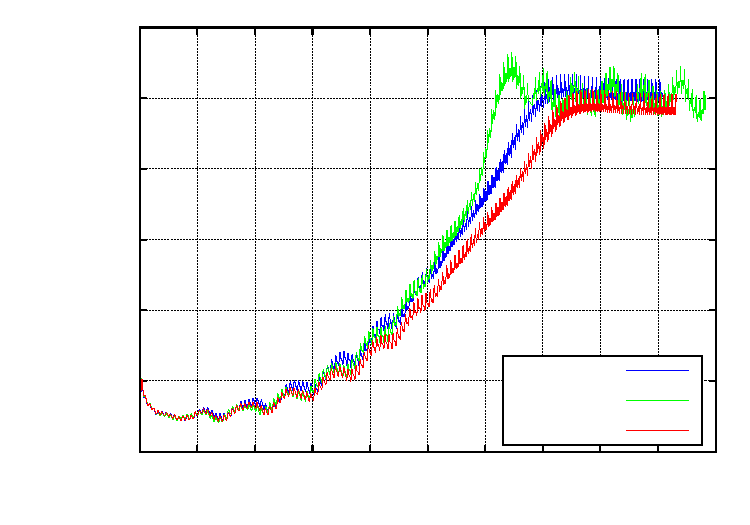
\includegraphics{RH2DNIRVANA}}%
    \gplfronttext
  \end{picture}%
\endgroup

	\end{center}
\caption{Alle 3 Codes aehneln sich bei der Exzentrizitaet, jedoch oszilliert FARGO nicht wie RH2D, nachdem die maximale Exzentrizitaet erreicht, und somit die Disk eingeschwungen ist. FARGO verhaelt sich in diesem Fall eher wie NIRVANA, auch wenn der Anstieg etwas steiler und das Maximum hoeher ist. Durch den exponentiellen Anstieg auf einen gewissen Wert der Exzentrizitaet sieht man, dass es sich um einen nichtexzentrischen Binaerstern handeln muss.
TODO: Setup von CVDisk}
\end {figure}

\section{Modellierung nicht-exzentrischer Binaersternsysteme: Parameterstudie: h, q}
Nun wollen wir betrachten, wie sich Scheiben verhalten, wenn der Binaerstern sich auf einer Kreisbahn um die Scheibe und den Primaerstern bewegt. Im Gegensatz zu einer exzentrischen Bahn sollte hier die Exzentrizitaet der Scheibe einen Endzustand erreichen. Wir gehen davon aus, dass die Exzentrizitaet mit einem exponentiellen Wachstum erreicht wird und diesen Wert dann beibehaelt. Wenn sich die Exzentrizitaet, nachdem sie ihr Maximum erreicht hat, langsam weiter veraendert, ist davon auszugehen, dass dies durch numerische Fehler bzw. den Code passiert.
Wir variieren die Parameter Aspectratio H/r, also die Dicke der Disk und den Parameter MassRatio q, das Massenverhältnis des Binärsterns zu dem Primärstern. 

Setup:

\begin{tabular}{|c|c|c|c|c|}
\hline$M_1 [\unit{\astrosun}]$ & $M_2$ [\unit{\astrosun}] & $\frac{H}{r}$ & a [$\unit{AU}$] & e \\\hline
1.0 & 0.1 - 1.0 & 0.03 - 0.05 & 1.0 & 0.0 \\\hline
\end{tabular}

Ziel ist es, die Wachstumsrate, sowie den Wert der Exzentrizität der Scheibe zu bestimmen. Als Randbedingungen verwenden wir innen reflektierende und aussen offene.
Wir betrachten auch die Präzession der Disk.

Probleme traten auf, wenn die kuenstliche Viskositaet nach von Neumann Richtmyer nicht aktiviert war. Dann werden die Berechnungszeitschritte extrem klein, die Rechnungen dauerten also ewig. Dazu gibt es partiell extrem hohe Geschwindigkeiten einzelner Zellen, was zu Exzentrizitaeten von weit ueber 1 fuehrt. Danach kollabiert die Exzentrizitaet der gesamten Scheibe auf 0 und steigt langsam wieder an. Der am Ende erreichte Wert entspricht den Ergebnissen mit CVNR, jedoch ist die Growth Rate anders.

\subsubsection{Lagrange-Punkte}
Fuer verschiedene Massenverhaeltnisse des Primaer- und Binaer-Sterns muss man verschiedene Scheibenradien waehlen, da der Maximalradius der Scheibe nur bis zu dem Lagrangepunkt $L_1$ Sinn macht. Der Lagrangepunkt $L_1$ ist der Punkt im Raum, in dem sich ein kleiner Körper (eine Zelle unserer Scheibe) im Gravitationsfeld von 2 großen Körpern (Primaer- und Binaerstern) in relativer Ruhe zu den beiden Körpern befindet. Bei verschiedenen Massen haben wir also verschiedene Lagrangepunkte. Der Lagrangepunkt befindet sich auf der Verbindungsgeraden des Primaer- und des Binaersterns. Wir waehlen als Maximalradius der Scheibe die jeweiligen Lagrangepunkte. Wenn wir die Scheibe also groesse machen wuerden, haetten wir sofort einen grossen Masseverlust. Um das Groessenverhaeltnis der Scheibe gleich zu halten, passen wir den Minimalradius jeder Disk an unser Ausgangsverhaeltnis von $\frac{0.7}{0.05}$ an.
\begin {figure}
	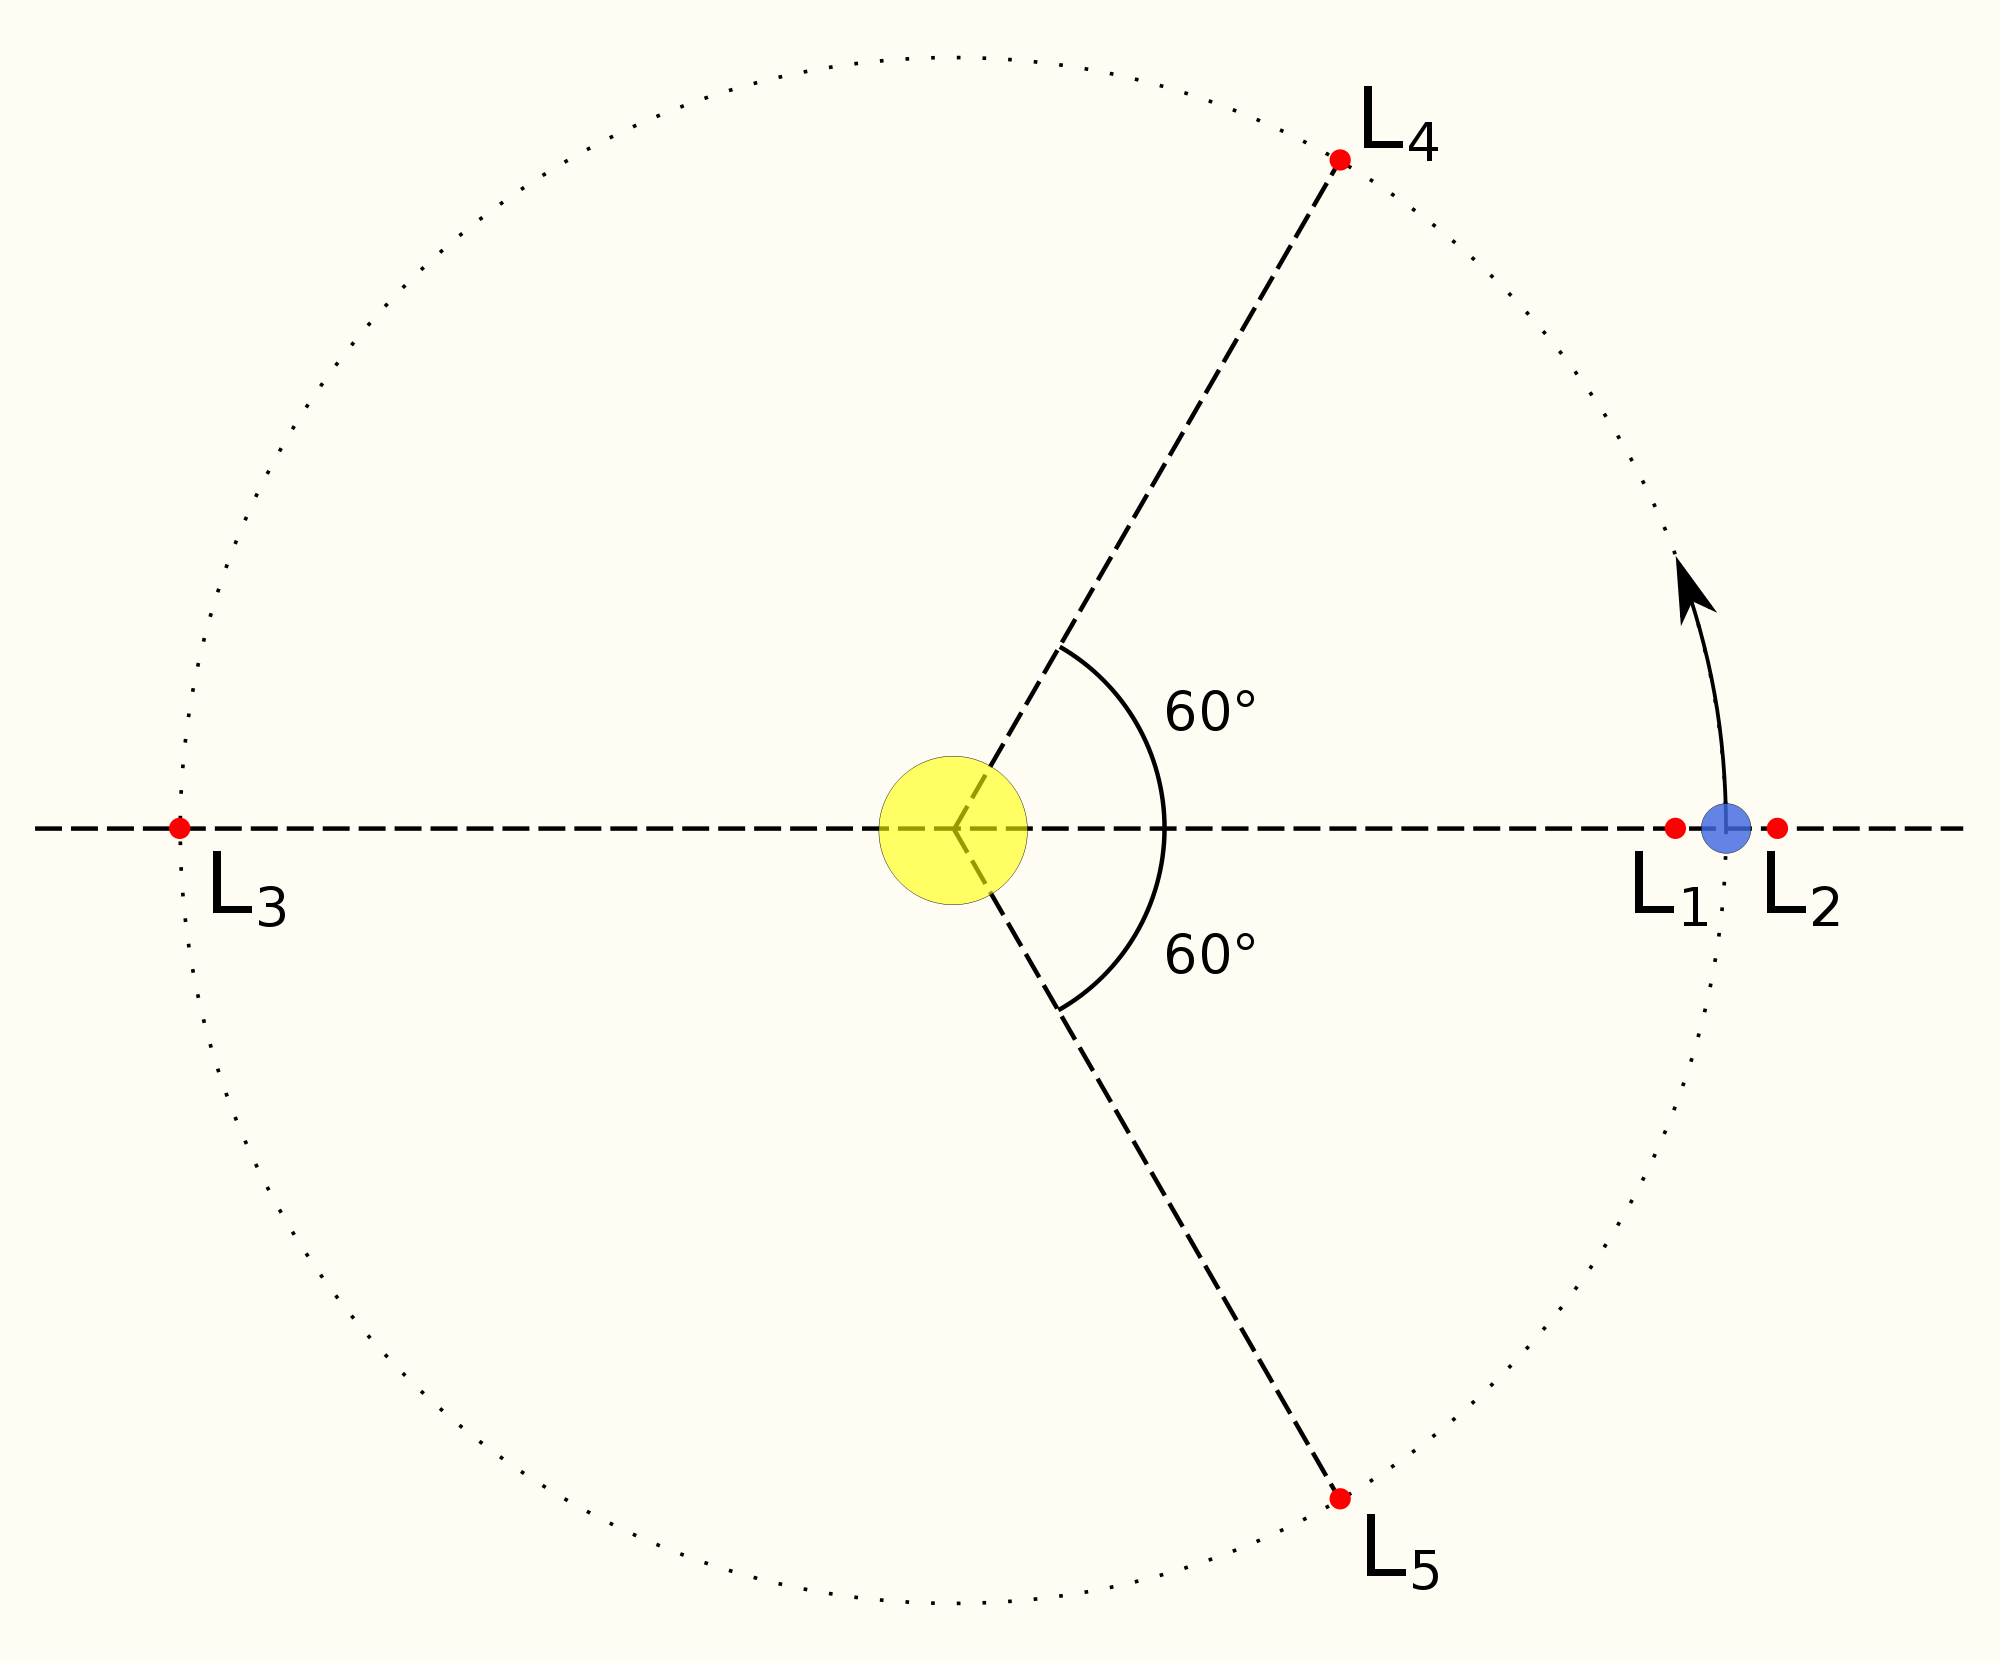
\includegraphics[scale=0.1]{2000px-Lagrange_very_massive.png}
\caption{Lagrange-Punkte: Sie lassen sich rechnerisch herleiten, wenn man die drei Massen auf einer Linie anordnet und für die Rotation um den gemeinsamen Schwerpunkt die Summe der Kräfte aus der Zentrifugalwirkung der Rotation um den gemeinsamen Schwerpunkt und aus der graviativen Anziehung untereinander zu Null setzt.}
\end {figure}

\begin{tabular}{|c|c|c|}
\hline q & Rmin [$\unit{AU}$] & Rmax [$\unit{AU}$]\\\hline
0.1	& 0.7175 & 0.05125\\\hline
0.2	& 0.6585 & 0.0470\\\hline
0.3	& 0.62087 & 0.0443\\\hline
0.4	& 0.0424 & 0.5929\\\hline
0.5	& 0.0407 & 0.5708\\\hline
0.6	& 0.0395 & 0.5523\\\hline
0.7	& 0.0383 & 0.5366\\\hline
0.8	& 0.03735 & 0.5229\\\hline
0.9	& 0.0365 & 0.5108\\\hline
1.0	& 0.0357 & 0.5\\\hline
\end{tabular}






\begin {figure}
	\begin{center}
		% GNUPLOT: LaTeX picture with Postscript
\begingroup
  \makeatletter
  \providecommand\color[2][]{%
    \GenericError{(gnuplot) \space\space\space\@spaces}{%
      Package color not loaded in conjunction with
      terminal option `colourtext'%
    }{See the gnuplot documentation for explanation.%
    }{Either use 'blacktext' in gnuplot or load the package
      color.sty in LaTeX.}%
    \renewcommand\color[2][]{}%
  }%
  \providecommand\includegraphics[2][]{%
    \GenericError{(gnuplot) \space\space\space\@spaces}{%
      Package graphicx or graphics not loaded%
    }{See the gnuplot documentation for explanation.%
    }{The gnuplot epslatex terminal needs graphicx.sty or graphics.sty.}%
    \renewcommand\includegraphics[2][]{}%
  }%
  \providecommand\rotatebox[2]{#2}%
  \@ifundefined{ifGPcolor}{%
    \newif\ifGPcolor
    \GPcolortrue
  }{}%
  \@ifundefined{ifGPblacktext}{%
    \newif\ifGPblacktext
    \GPblacktexttrue
  }{}%
  % define a \g@addto@macro without @ in the name:
  \let\gplgaddtomacro\g@addto@macro
  % define empty templates for all commands taking text:
  \gdef\gplbacktext{}%
  \gdef\gplfronttext{}%
  \makeatother
  \ifGPblacktext
    % no textcolor at all
    \def\colorrgb#1{}%
    \def\colorgray#1{}%
  \else
    % gray or color?
    \ifGPcolor
      \def\colorrgb#1{\color[rgb]{#1}}%
      \def\colorgray#1{\color[gray]{#1}}%
      \expandafter\def\csname LTw\endcsname{\color{white}}%
      \expandafter\def\csname LTb\endcsname{\color{black}}%
      \expandafter\def\csname LTa\endcsname{\color{black}}%
      \expandafter\def\csname LT0\endcsname{\color[rgb]{1,0,0}}%
      \expandafter\def\csname LT1\endcsname{\color[rgb]{0,1,0}}%
      \expandafter\def\csname LT2\endcsname{\color[rgb]{0,0,1}}%
      \expandafter\def\csname LT3\endcsname{\color[rgb]{1,0,1}}%
      \expandafter\def\csname LT4\endcsname{\color[rgb]{0,1,1}}%
      \expandafter\def\csname LT5\endcsname{\color[rgb]{1,1,0}}%
      \expandafter\def\csname LT6\endcsname{\color[rgb]{0,0,0}}%
      \expandafter\def\csname LT7\endcsname{\color[rgb]{1,0.3,0}}%
      \expandafter\def\csname LT8\endcsname{\color[rgb]{0.5,0.5,0.5}}%
    \else
      % gray
      \def\colorrgb#1{\color{black}}%
      \def\colorgray#1{\color[gray]{#1}}%
      \expandafter\def\csname LTw\endcsname{\color{white}}%
      \expandafter\def\csname LTb\endcsname{\color{black}}%
      \expandafter\def\csname LTa\endcsname{\color{black}}%
      \expandafter\def\csname LT0\endcsname{\color{black}}%
      \expandafter\def\csname LT1\endcsname{\color{black}}%
      \expandafter\def\csname LT2\endcsname{\color{black}}%
      \expandafter\def\csname LT3\endcsname{\color{black}}%
      \expandafter\def\csname LT4\endcsname{\color{black}}%
      \expandafter\def\csname LT5\endcsname{\color{black}}%
      \expandafter\def\csname LT6\endcsname{\color{black}}%
      \expandafter\def\csname LT7\endcsname{\color{black}}%
      \expandafter\def\csname LT8\endcsname{\color{black}}%
    \fi
  \fi
  \setlength{\unitlength}{0.0500bp}%
  \begin{picture}(7200.00,5040.00)%
    \gplgaddtomacro\gplbacktext{%
      \csname LTb\endcsname%
      \put(1210,704){\makebox(0,0)[r]{\strut{} 0}}%
      \csname LTb\endcsname%
      \put(1210,1317){\makebox(0,0)[r]{\strut{} 0.1}}%
      \csname LTb\endcsname%
      \put(1210,1929){\makebox(0,0)[r]{\strut{} 0.2}}%
      \csname LTb\endcsname%
      \put(1210,2542){\makebox(0,0)[r]{\strut{} 0.3}}%
      \csname LTb\endcsname%
      \put(1210,3155){\makebox(0,0)[r]{\strut{} 0.4}}%
      \csname LTb\endcsname%
      \put(1210,3767){\makebox(0,0)[r]{\strut{} 0.5}}%
      \csname LTb\endcsname%
      \put(1210,4380){\makebox(0,0)[r]{\strut{} 0.6}}%
      \csname LTb\endcsname%
      \put(1342,484){\makebox(0,0){\strut{} 0}}%
      \csname LTb\endcsname%
      \put(2033,484){\makebox(0,0){\strut{} 20}}%
      \csname LTb\endcsname%
      \put(2724,484){\makebox(0,0){\strut{} 40}}%
      \csname LTb\endcsname%
      \put(3415,484){\makebox(0,0){\strut{} 60}}%
      \csname LTb\endcsname%
      \put(4106,484){\makebox(0,0){\strut{} 80}}%
      \csname LTb\endcsname%
      \put(4797,484){\makebox(0,0){\strut{} 100}}%
      \csname LTb\endcsname%
      \put(5488,484){\makebox(0,0){\strut{} 120}}%
      \csname LTb\endcsname%
      \put(6179,484){\makebox(0,0){\strut{} 140}}%
      \csname LTb\endcsname%
      \put(6870,484){\makebox(0,0){\strut{} 160}}%
      \put(440,2542){\rotatebox{90}{\makebox(0,0){\strut{}Eccentricity}}}%
      \put(4106,154){\makebox(0,0){\strut{}Time [Years]}}%
      \put(4106,4710){\makebox(0,0){\strut{}h = 0.05}}%
    }%
    \gplgaddtomacro\gplfronttext{%
      \csname LTb\endcsname%
      \put(5883,3484){\makebox(0,0)[r]{\strut{}q=0.1}}%
      \csname LTb\endcsname%
      \put(5883,3198){\makebox(0,0)[r]{\strut{}q=0.2}}%
      \csname LTb\endcsname%
      \put(5883,2912){\makebox(0,0)[r]{\strut{}q=0.3}}%
      \csname LTb\endcsname%
      \put(5883,2626){\makebox(0,0)[r]{\strut{}q=0.6}}%
      \csname LTb\endcsname%
      \put(5883,2340){\makebox(0,0)[r]{\strut{}q=0.4}}%
      \csname LTb\endcsname%
      \put(5883,2054){\makebox(0,0)[r]{\strut{}q=0.5}}%
      \csname LTb\endcsname%
      \put(5883,1768){\makebox(0,0)[r]{\strut{}q=0.7}}%
      \csname LTb\endcsname%
      \put(5883,1482){\makebox(0,0)[r]{\strut{}q=0.8}}%
      \csname LTb\endcsname%
      \put(5883,1196){\makebox(0,0)[r]{\strut{}q=0.9}}%
      \csname LTb\endcsname%
      \put(5883,910){\makebox(0,0)[r]{\strut{}q=1.0}}%
    }%
    \gplbacktext
    \put(0,0){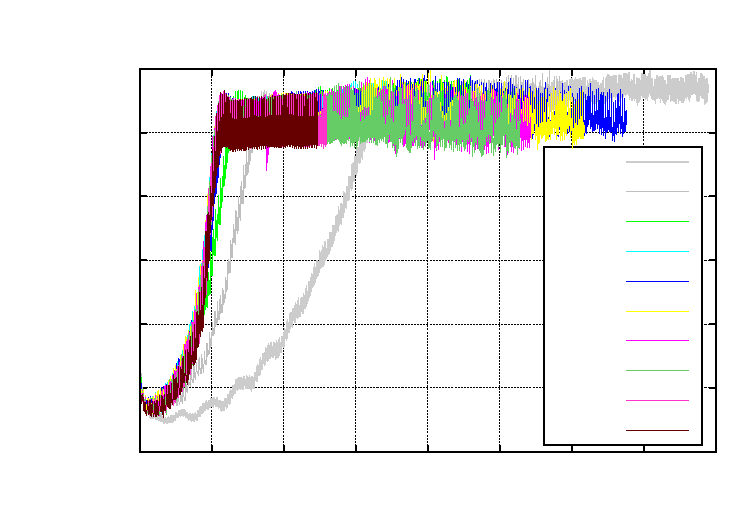
\includegraphics{diskeccentricityh005}}%
    \gplfronttext
  \end{picture}%
\endgroup

	\end{center}
\caption{Der schnellste Anstieg der Exzentrizitaet ist bei $q = 0.3$ und $q = 0.4$}
\end {figure}
\begin {figure}
	\begin{center}
		% GNUPLOT: LaTeX picture with Postscript
\begingroup
  \makeatletter
  \providecommand\color[2][]{%
    \GenericError{(gnuplot) \space\space\space\@spaces}{%
      Package color not loaded in conjunction with
      terminal option `colourtext'%
    }{See the gnuplot documentation for explanation.%
    }{Either use 'blacktext' in gnuplot or load the package
      color.sty in LaTeX.}%
    \renewcommand\color[2][]{}%
  }%
  \providecommand\includegraphics[2][]{%
    \GenericError{(gnuplot) \space\space\space\@spaces}{%
      Package graphicx or graphics not loaded%
    }{See the gnuplot documentation for explanation.%
    }{The gnuplot epslatex terminal needs graphicx.sty or graphics.sty.}%
    \renewcommand\includegraphics[2][]{}%
  }%
  \providecommand\rotatebox[2]{#2}%
  \@ifundefined{ifGPcolor}{%
    \newif\ifGPcolor
    \GPcolortrue
  }{}%
  \@ifundefined{ifGPblacktext}{%
    \newif\ifGPblacktext
    \GPblacktexttrue
  }{}%
  % define a \g@addto@macro without @ in the name:
  \let\gplgaddtomacro\g@addto@macro
  % define empty templates for all commands taking text:
  \gdef\gplbacktext{}%
  \gdef\gplfronttext{}%
  \makeatother
  \ifGPblacktext
    % no textcolor at all
    \def\colorrgb#1{}%
    \def\colorgray#1{}%
  \else
    % gray or color?
    \ifGPcolor
      \def\colorrgb#1{\color[rgb]{#1}}%
      \def\colorgray#1{\color[gray]{#1}}%
      \expandafter\def\csname LTw\endcsname{\color{white}}%
      \expandafter\def\csname LTb\endcsname{\color{black}}%
      \expandafter\def\csname LTa\endcsname{\color{black}}%
      \expandafter\def\csname LT0\endcsname{\color[rgb]{1,0,0}}%
      \expandafter\def\csname LT1\endcsname{\color[rgb]{0,1,0}}%
      \expandafter\def\csname LT2\endcsname{\color[rgb]{0,0,1}}%
      \expandafter\def\csname LT3\endcsname{\color[rgb]{1,0,1}}%
      \expandafter\def\csname LT4\endcsname{\color[rgb]{0,1,1}}%
      \expandafter\def\csname LT5\endcsname{\color[rgb]{1,1,0}}%
      \expandafter\def\csname LT6\endcsname{\color[rgb]{0,0,0}}%
      \expandafter\def\csname LT7\endcsname{\color[rgb]{1,0.3,0}}%
      \expandafter\def\csname LT8\endcsname{\color[rgb]{0.5,0.5,0.5}}%
    \else
      % gray
      \def\colorrgb#1{\color{black}}%
      \def\colorgray#1{\color[gray]{#1}}%
      \expandafter\def\csname LTw\endcsname{\color{white}}%
      \expandafter\def\csname LTb\endcsname{\color{black}}%
      \expandafter\def\csname LTa\endcsname{\color{black}}%
      \expandafter\def\csname LT0\endcsname{\color{black}}%
      \expandafter\def\csname LT1\endcsname{\color{black}}%
      \expandafter\def\csname LT2\endcsname{\color{black}}%
      \expandafter\def\csname LT3\endcsname{\color{black}}%
      \expandafter\def\csname LT4\endcsname{\color{black}}%
      \expandafter\def\csname LT5\endcsname{\color{black}}%
      \expandafter\def\csname LT6\endcsname{\color{black}}%
      \expandafter\def\csname LT7\endcsname{\color{black}}%
      \expandafter\def\csname LT8\endcsname{\color{black}}%
    \fi
  \fi
  \setlength{\unitlength}{0.0500bp}%
  \begin{picture}(7200.00,5040.00)%
    \gplgaddtomacro\gplbacktext{%
      \csname LTb\endcsname%
      \put(1474,704){\makebox(0,0)[r]{\strut{} 0.001}}%
      \csname LTb\endcsname%
      \put(1474,1929){\makebox(0,0)[r]{\strut{} 0.01}}%
      \csname LTb\endcsname%
      \put(1474,3155){\makebox(0,0)[r]{\strut{} 0.1}}%
      \csname LTb\endcsname%
      \put(1474,4380){\makebox(0,0)[r]{\strut{} 1}}%
      \csname LTb\endcsname%
      \put(1606,484){\makebox(0,0){\strut{} 0}}%
      \csname LTb\endcsname%
      \put(2264,484){\makebox(0,0){\strut{} 20}}%
      \csname LTb\endcsname%
      \put(2922,484){\makebox(0,0){\strut{} 40}}%
      \csname LTb\endcsname%
      \put(3580,484){\makebox(0,0){\strut{} 60}}%
      \csname LTb\endcsname%
      \put(4238,484){\makebox(0,0){\strut{} 80}}%
      \csname LTb\endcsname%
      \put(4896,484){\makebox(0,0){\strut{} 100}}%
      \csname LTb\endcsname%
      \put(5554,484){\makebox(0,0){\strut{} 120}}%
      \csname LTb\endcsname%
      \put(6212,484){\makebox(0,0){\strut{} 140}}%
      \csname LTb\endcsname%
      \put(6870,484){\makebox(0,0){\strut{} 160}}%
      \put(440,2542){\rotatebox{90}{\makebox(0,0){\strut{}Eccentricity}}}%
      \put(4238,154){\makebox(0,0){\strut{}Time [Years]}}%
      \put(4238,4710){\makebox(0,0){\strut{}h = 0.04}}%
    }%
    \gplgaddtomacro\gplfronttext{%
      \csname LTb\endcsname%
      \put(5883,3484){\makebox(0,0)[r]{\strut{}q=0.7}}%
      \csname LTb\endcsname%
      \put(5883,3198){\makebox(0,0)[r]{\strut{}q=0.1}}%
      \csname LTb\endcsname%
      \put(5883,2912){\makebox(0,0)[r]{\strut{}q=0.3}}%
      \csname LTb\endcsname%
      \put(5883,2626){\makebox(0,0)[r]{\strut{}q=0.6}}%
      \csname LTb\endcsname%
      \put(5883,2340){\makebox(0,0)[r]{\strut{}q=0.4}}%
      \csname LTb\endcsname%
      \put(5883,2054){\makebox(0,0)[r]{\strut{}q=0.5}}%
      \csname LTb\endcsname%
      \put(5883,1768){\makebox(0,0)[r]{\strut{}q=0.2}}%
      \csname LTb\endcsname%
      \put(5883,1482){\makebox(0,0)[r]{\strut{}q=0.8}}%
      \csname LTb\endcsname%
      \put(5883,1196){\makebox(0,0)[r]{\strut{}q=0.9}}%
      \csname LTb\endcsname%
      \put(5883,910){\makebox(0,0)[r]{\strut{}q=1.0}}%
    }%
    \gplbacktext
    \put(0,0){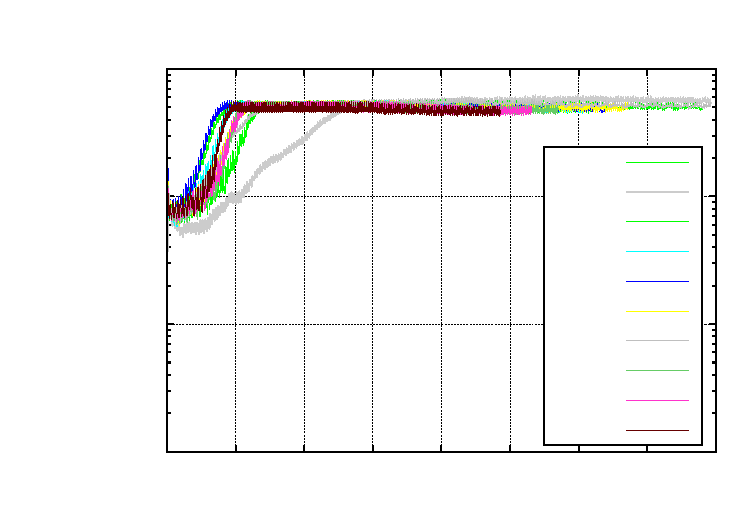
\includegraphics{diskeccentricityh004}}%
    \gplfronttext
  \end{picture}%
\endgroup

	\end{center}
\end {figure}
\begin {figure}
	\begin{center}
		% GNUPLOT: LaTeX picture with Postscript
\begingroup
  \makeatletter
  \providecommand\color[2][]{%
    \GenericError{(gnuplot) \space\space\space\@spaces}{%
      Package color not loaded in conjunction with
      terminal option `colourtext'%
    }{See the gnuplot documentation for explanation.%
    }{Either use 'blacktext' in gnuplot or load the package
      color.sty in LaTeX.}%
    \renewcommand\color[2][]{}%
  }%
  \providecommand\includegraphics[2][]{%
    \GenericError{(gnuplot) \space\space\space\@spaces}{%
      Package graphicx or graphics not loaded%
    }{See the gnuplot documentation for explanation.%
    }{The gnuplot epslatex terminal needs graphicx.sty or graphics.sty.}%
    \renewcommand\includegraphics[2][]{}%
  }%
  \providecommand\rotatebox[2]{#2}%
  \@ifundefined{ifGPcolor}{%
    \newif\ifGPcolor
    \GPcolortrue
  }{}%
  \@ifundefined{ifGPblacktext}{%
    \newif\ifGPblacktext
    \GPblacktexttrue
  }{}%
  % define a \g@addto@macro without @ in the name:
  \let\gplgaddtomacro\g@addto@macro
  % define empty templates for all commands taking text:
  \gdef\gplbacktext{}%
  \gdef\gplfronttext{}%
  \makeatother
  \ifGPblacktext
    % no textcolor at all
    \def\colorrgb#1{}%
    \def\colorgray#1{}%
  \else
    % gray or color?
    \ifGPcolor
      \def\colorrgb#1{\color[rgb]{#1}}%
      \def\colorgray#1{\color[gray]{#1}}%
      \expandafter\def\csname LTw\endcsname{\color{white}}%
      \expandafter\def\csname LTb\endcsname{\color{black}}%
      \expandafter\def\csname LTa\endcsname{\color{black}}%
      \expandafter\def\csname LT0\endcsname{\color[rgb]{1,0,0}}%
      \expandafter\def\csname LT1\endcsname{\color[rgb]{0,1,0}}%
      \expandafter\def\csname LT2\endcsname{\color[rgb]{0,0,1}}%
      \expandafter\def\csname LT3\endcsname{\color[rgb]{1,0,1}}%
      \expandafter\def\csname LT4\endcsname{\color[rgb]{0,1,1}}%
      \expandafter\def\csname LT5\endcsname{\color[rgb]{1,1,0}}%
      \expandafter\def\csname LT6\endcsname{\color[rgb]{0,0,0}}%
      \expandafter\def\csname LT7\endcsname{\color[rgb]{1,0.3,0}}%
      \expandafter\def\csname LT8\endcsname{\color[rgb]{0.5,0.5,0.5}}%
    \else
      % gray
      \def\colorrgb#1{\color{black}}%
      \def\colorgray#1{\color[gray]{#1}}%
      \expandafter\def\csname LTw\endcsname{\color{white}}%
      \expandafter\def\csname LTb\endcsname{\color{black}}%
      \expandafter\def\csname LTa\endcsname{\color{black}}%
      \expandafter\def\csname LT0\endcsname{\color{black}}%
      \expandafter\def\csname LT1\endcsname{\color{black}}%
      \expandafter\def\csname LT2\endcsname{\color{black}}%
      \expandafter\def\csname LT3\endcsname{\color{black}}%
      \expandafter\def\csname LT4\endcsname{\color{black}}%
      \expandafter\def\csname LT5\endcsname{\color{black}}%
      \expandafter\def\csname LT6\endcsname{\color{black}}%
      \expandafter\def\csname LT7\endcsname{\color{black}}%
      \expandafter\def\csname LT8\endcsname{\color{black}}%
    \fi
  \fi
  \setlength{\unitlength}{0.0500bp}%
  \begin{picture}(7200.00,5040.00)%
    \gplgaddtomacro\gplbacktext{%
      \csname LTb\endcsname%
      \put(1210,704){\makebox(0,0)[r]{\strut{} 0}}%
      \csname LTb\endcsname%
      \put(1210,1317){\makebox(0,0)[r]{\strut{} 0.1}}%
      \csname LTb\endcsname%
      \put(1210,1929){\makebox(0,0)[r]{\strut{} 0.2}}%
      \csname LTb\endcsname%
      \put(1210,2542){\makebox(0,0)[r]{\strut{} 0.3}}%
      \csname LTb\endcsname%
      \put(1210,3155){\makebox(0,0)[r]{\strut{} 0.4}}%
      \csname LTb\endcsname%
      \put(1210,3767){\makebox(0,0)[r]{\strut{} 0.5}}%
      \csname LTb\endcsname%
      \put(1210,4380){\makebox(0,0)[r]{\strut{} 0.6}}%
      \csname LTb\endcsname%
      \put(1342,484){\makebox(0,0){\strut{} 0}}%
      \csname LTb\endcsname%
      \put(2192,484){\makebox(0,0){\strut{} 10}}%
      \csname LTb\endcsname%
      \put(3043,484){\makebox(0,0){\strut{} 20}}%
      \csname LTb\endcsname%
      \put(3893,484){\makebox(0,0){\strut{} 30}}%
      \csname LTb\endcsname%
      \put(4744,484){\makebox(0,0){\strut{} 40}}%
      \csname LTb\endcsname%
      \put(5594,484){\makebox(0,0){\strut{} 50}}%
      \csname LTb\endcsname%
      \put(6445,484){\makebox(0,0){\strut{} 60}}%
      \put(440,2542){\rotatebox{90}{\makebox(0,0){\strut{}Eccentricity}}}%
      \put(4106,154){\makebox(0,0){\strut{}Time [Years]}}%
      \put(4106,4710){\makebox(0,0){\strut{}h = 0.03}}%
    }%
    \gplgaddtomacro\gplfronttext{%
      \csname LTb\endcsname%
      \put(5883,1812){\makebox(0,0)[r]{\strut{}q=0.1}}%
      \csname LTb\endcsname%
      \put(5883,1702){\makebox(0,0)[r]{\strut{}q=0.2}}%
      \csname LTb\endcsname%
      \put(5883,1592){\makebox(0,0)[r]{\strut{}q=0.3}}%
      \csname LTb\endcsname%
      \put(5883,1482){\makebox(0,0)[r]{\strut{}q=0.6}}%
      \csname LTb\endcsname%
      \put(5883,1372){\makebox(0,0)[r]{\strut{}q=0.4}}%
      \csname LTb\endcsname%
      \put(5883,1262){\makebox(0,0)[r]{\strut{}q=0.5}}%
      \csname LTb\endcsname%
      \put(5883,1152){\makebox(0,0)[r]{\strut{}q=0.7}}%
      \csname LTb\endcsname%
      \put(5883,1042){\makebox(0,0)[r]{\strut{}q=0.8}}%
      \csname LTb\endcsname%
      \put(5883,932){\makebox(0,0)[r]{\strut{}q=0.9}}%
      \csname LTb\endcsname%
      \put(5883,822){\makebox(0,0)[r]{\strut{}q=1.0}}%
    }%
    \gplbacktext
    \put(0,0){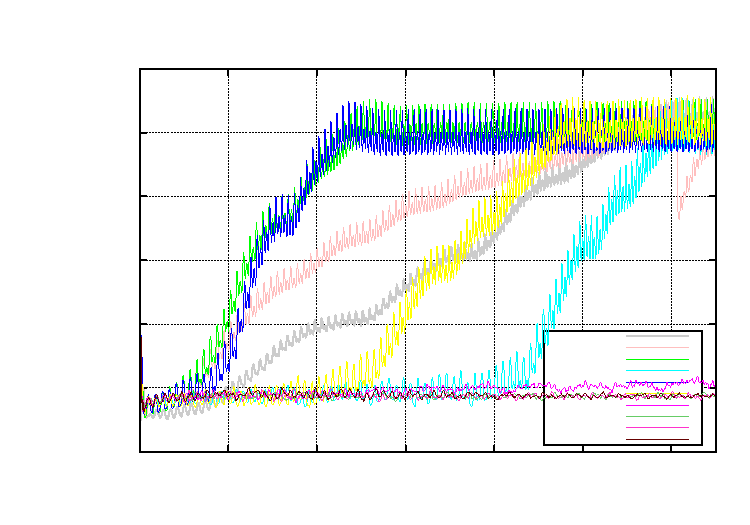
\includegraphics{diskeccentricityh003}}%
    \gplfronttext
  \end{picture}%
\endgroup

	\end{center}
\end {figure}

\subsection{Periastron}
\subsubsection{h = 0.05}
\clearpage
\begin {figure}
	\begin{center}
		% GNUPLOT: LaTeX picture with Postscript
\begingroup
  \makeatletter
  \providecommand\color[2][]{%
    \GenericError{(gnuplot) \space\space\space\@spaces}{%
      Package color not loaded in conjunction with
      terminal option `colourtext'%
    }{See the gnuplot documentation for explanation.%
    }{Either use 'blacktext' in gnuplot or load the package
      color.sty in LaTeX.}%
    \renewcommand\color[2][]{}%
  }%
  \providecommand\includegraphics[2][]{%
    \GenericError{(gnuplot) \space\space\space\@spaces}{%
      Package graphicx or graphics not loaded%
    }{See the gnuplot documentation for explanation.%
    }{The gnuplot epslatex terminal needs graphicx.sty or graphics.sty.}%
    \renewcommand\includegraphics[2][]{}%
  }%
  \providecommand\rotatebox[2]{#2}%
  \@ifundefined{ifGPcolor}{%
    \newif\ifGPcolor
    \GPcolortrue
  }{}%
  \@ifundefined{ifGPblacktext}{%
    \newif\ifGPblacktext
    \GPblacktexttrue
  }{}%
  % define a \g@addto@macro without @ in the name:
  \let\gplgaddtomacro\g@addto@macro
  % define empty templates for all commands taking text:
  \gdef\gplbacktext{}%
  \gdef\gplfronttext{}%
  \makeatother
  \ifGPblacktext
    % no textcolor at all
    \def\colorrgb#1{}%
    \def\colorgray#1{}%
  \else
    % gray or color?
    \ifGPcolor
      \def\colorrgb#1{\color[rgb]{#1}}%
      \def\colorgray#1{\color[gray]{#1}}%
      \expandafter\def\csname LTw\endcsname{\color{white}}%
      \expandafter\def\csname LTb\endcsname{\color{black}}%
      \expandafter\def\csname LTa\endcsname{\color{black}}%
      \expandafter\def\csname LT0\endcsname{\color[rgb]{1,0,0}}%
      \expandafter\def\csname LT1\endcsname{\color[rgb]{0,1,0}}%
      \expandafter\def\csname LT2\endcsname{\color[rgb]{0,0,1}}%
      \expandafter\def\csname LT3\endcsname{\color[rgb]{1,0,1}}%
      \expandafter\def\csname LT4\endcsname{\color[rgb]{0,1,1}}%
      \expandafter\def\csname LT5\endcsname{\color[rgb]{1,1,0}}%
      \expandafter\def\csname LT6\endcsname{\color[rgb]{0,0,0}}%
      \expandafter\def\csname LT7\endcsname{\color[rgb]{1,0.3,0}}%
      \expandafter\def\csname LT8\endcsname{\color[rgb]{0.5,0.5,0.5}}%
    \else
      % gray
      \def\colorrgb#1{\color{black}}%
      \def\colorgray#1{\color[gray]{#1}}%
      \expandafter\def\csname LTw\endcsname{\color{white}}%
      \expandafter\def\csname LTb\endcsname{\color{black}}%
      \expandafter\def\csname LTa\endcsname{\color{black}}%
      \expandafter\def\csname LT0\endcsname{\color{black}}%
      \expandafter\def\csname LT1\endcsname{\color{black}}%
      \expandafter\def\csname LT2\endcsname{\color{black}}%
      \expandafter\def\csname LT3\endcsname{\color{black}}%
      \expandafter\def\csname LT4\endcsname{\color{black}}%
      \expandafter\def\csname LT5\endcsname{\color{black}}%
      \expandafter\def\csname LT6\endcsname{\color{black}}%
      \expandafter\def\csname LT7\endcsname{\color{black}}%
      \expandafter\def\csname LT8\endcsname{\color{black}}%
    \fi
  \fi
  \setlength{\unitlength}{0.0500bp}%
  \begin{picture}(8640.00,4032.00)%
    \gplgaddtomacro\gplbacktext{%
      \csname LTb\endcsname%
      \put(1210,704){\makebox(0,0)[r]{\strut{} 0.4}}%
      \csname LTb\endcsname%
      \put(1210,1085){\makebox(0,0)[r]{\strut{} 0.5}}%
      \csname LTb\endcsname%
      \put(1210,1466){\makebox(0,0)[r]{\strut{} 0.6}}%
      \csname LTb\endcsname%
      \put(1210,1847){\makebox(0,0)[r]{\strut{} 0.7}}%
      \csname LTb\endcsname%
      \put(1210,2229){\makebox(0,0)[r]{\strut{} 0.8}}%
      \csname LTb\endcsname%
      \put(1210,2610){\makebox(0,0)[r]{\strut{} 0.9}}%
      \csname LTb\endcsname%
      \put(1210,2991){\makebox(0,0)[r]{\strut{} 1}}%
      \csname LTb\endcsname%
      \put(1210,3372){\makebox(0,0)[r]{\strut{} 1.1}}%
      \csname LTb\endcsname%
      \put(1342,484){\makebox(0,0){\strut{} 0.1}}%
      \csname LTb\endcsname%
      \put(2116,484){\makebox(0,0){\strut{} 0.2}}%
      \csname LTb\endcsname%
      \put(2890,484){\makebox(0,0){\strut{} 0.3}}%
      \csname LTb\endcsname%
      \put(3665,484){\makebox(0,0){\strut{} 0.4}}%
      \csname LTb\endcsname%
      \put(4439,484){\makebox(0,0){\strut{} 0.5}}%
      \csname LTb\endcsname%
      \put(5213,484){\makebox(0,0){\strut{} 0.6}}%
      \csname LTb\endcsname%
      \put(5987,484){\makebox(0,0){\strut{} 0.7}}%
      \csname LTb\endcsname%
      \put(6762,484){\makebox(0,0){\strut{} 0.8}}%
      \csname LTb\endcsname%
      \put(7536,484){\makebox(0,0){\strut{} 0.9}}%
      \csname LTb\endcsname%
      \put(8310,484){\makebox(0,0){\strut{} 1}}%
      \put(440,2038){\rotatebox{90}{\makebox(0,0){\strut{}$\bar{\omega}$}}}%
      \put(4826,154){\makebox(0,0){\strut{}q}}%
      \put(4826,3702){\makebox(0,0){\strut{}h = 0.05}}%
    }%
    \gplgaddtomacro\gplfronttext{%
      \csname LTb\endcsname%
      \put(7323,855){\makebox(0,0)[r]{\strut{}$\bar{\omega}$}}%
    }%
    \gplbacktext
    \put(0,0){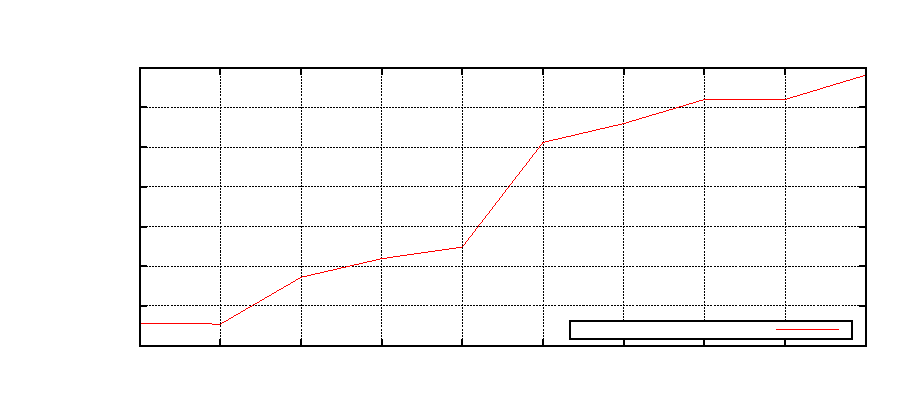
\includegraphics{diskperih005}}%
    \gplfronttext
  \end{picture}%
\endgroup

	\end{center}
	\caption{Mit zunehmendem MassRatio praezediert die Disk schneller}
\end {figure}

\clearpage
\begin {figure}
	\begin{center}
		% GNUPLOT: LaTeX picture with Postscript
\begingroup
  \makeatletter
  \providecommand\color[2][]{%
    \GenericError{(gnuplot) \space\space\space\@spaces}{%
      Package color not loaded in conjunction with
      terminal option `colourtext'%
    }{See the gnuplot documentation for explanation.%
    }{Either use 'blacktext' in gnuplot or load the package
      color.sty in LaTeX.}%
    \renewcommand\color[2][]{}%
  }%
  \providecommand\includegraphics[2][]{%
    \GenericError{(gnuplot) \space\space\space\@spaces}{%
      Package graphicx or graphics not loaded%
    }{See the gnuplot documentation for explanation.%
    }{The gnuplot epslatex terminal needs graphicx.sty or graphics.sty.}%
    \renewcommand\includegraphics[2][]{}%
  }%
  \providecommand\rotatebox[2]{#2}%
  \@ifundefined{ifGPcolor}{%
    \newif\ifGPcolor
    \GPcolortrue
  }{}%
  \@ifundefined{ifGPblacktext}{%
    \newif\ifGPblacktext
    \GPblacktexttrue
  }{}%
  % define a \g@addto@macro without @ in the name:
  \let\gplgaddtomacro\g@addto@macro
  % define empty templates for all commands taking text:
  \gdef\gplbacktext{}%
  \gdef\gplfronttext{}%
  \makeatother
  \ifGPblacktext
    % no textcolor at all
    \def\colorrgb#1{}%
    \def\colorgray#1{}%
  \else
    % gray or color?
    \ifGPcolor
      \def\colorrgb#1{\color[rgb]{#1}}%
      \def\colorgray#1{\color[gray]{#1}}%
      \expandafter\def\csname LTw\endcsname{\color{white}}%
      \expandafter\def\csname LTb\endcsname{\color{black}}%
      \expandafter\def\csname LTa\endcsname{\color{black}}%
      \expandafter\def\csname LT0\endcsname{\color[rgb]{1,0,0}}%
      \expandafter\def\csname LT1\endcsname{\color[rgb]{0,1,0}}%
      \expandafter\def\csname LT2\endcsname{\color[rgb]{0,0,1}}%
      \expandafter\def\csname LT3\endcsname{\color[rgb]{1,0,1}}%
      \expandafter\def\csname LT4\endcsname{\color[rgb]{0,1,1}}%
      \expandafter\def\csname LT5\endcsname{\color[rgb]{1,1,0}}%
      \expandafter\def\csname LT6\endcsname{\color[rgb]{0,0,0}}%
      \expandafter\def\csname LT7\endcsname{\color[rgb]{1,0.3,0}}%
      \expandafter\def\csname LT8\endcsname{\color[rgb]{0.5,0.5,0.5}}%
    \else
      % gray
      \def\colorrgb#1{\color{black}}%
      \def\colorgray#1{\color[gray]{#1}}%
      \expandafter\def\csname LTw\endcsname{\color{white}}%
      \expandafter\def\csname LTb\endcsname{\color{black}}%
      \expandafter\def\csname LTa\endcsname{\color{black}}%
      \expandafter\def\csname LT0\endcsname{\color{black}}%
      \expandafter\def\csname LT1\endcsname{\color{black}}%
      \expandafter\def\csname LT2\endcsname{\color{black}}%
      \expandafter\def\csname LT3\endcsname{\color{black}}%
      \expandafter\def\csname LT4\endcsname{\color{black}}%
      \expandafter\def\csname LT5\endcsname{\color{black}}%
      \expandafter\def\csname LT6\endcsname{\color{black}}%
      \expandafter\def\csname LT7\endcsname{\color{black}}%
      \expandafter\def\csname LT8\endcsname{\color{black}}%
    \fi
  \fi
  \setlength{\unitlength}{0.0500bp}%
  \begin{picture}(7200.00,5040.00)%
    \gplgaddtomacro\gplbacktext{%
      \csname LTb\endcsname%
      \put(1474,704){\makebox(0,0)[r]{\strut{} 0.01}}%
      \csname LTb\endcsname%
      \put(1474,1164){\makebox(0,0)[r]{\strut{} 0.015}}%
      \csname LTb\endcsname%
      \put(1474,1623){\makebox(0,0)[r]{\strut{} 0.02}}%
      \csname LTb\endcsname%
      \put(1474,2083){\makebox(0,0)[r]{\strut{} 0.025}}%
      \csname LTb\endcsname%
      \put(1474,2542){\makebox(0,0)[r]{\strut{} 0.03}}%
      \csname LTb\endcsname%
      \put(1474,3002){\makebox(0,0)[r]{\strut{} 0.035}}%
      \csname LTb\endcsname%
      \put(1474,3461){\makebox(0,0)[r]{\strut{} 0.04}}%
      \csname LTb\endcsname%
      \put(1474,3920){\makebox(0,0)[r]{\strut{} 0.045}}%
      \csname LTb\endcsname%
      \put(1474,4380){\makebox(0,0)[r]{\strut{} 0.05}}%
      \csname LTb\endcsname%
      \put(1606,484){\makebox(0,0){\strut{} 0.1}}%
      \csname LTb\endcsname%
      \put(2191,484){\makebox(0,0){\strut{} 0.2}}%
      \csname LTb\endcsname%
      \put(2776,484){\makebox(0,0){\strut{} 0.3}}%
      \csname LTb\endcsname%
      \put(3361,484){\makebox(0,0){\strut{} 0.4}}%
      \csname LTb\endcsname%
      \put(3946,484){\makebox(0,0){\strut{} 0.5}}%
      \csname LTb\endcsname%
      \put(4530,484){\makebox(0,0){\strut{} 0.6}}%
      \csname LTb\endcsname%
      \put(5115,484){\makebox(0,0){\strut{} 0.7}}%
      \csname LTb\endcsname%
      \put(5700,484){\makebox(0,0){\strut{} 0.8}}%
      \csname LTb\endcsname%
      \put(6285,484){\makebox(0,0){\strut{} 0.9}}%
      \csname LTb\endcsname%
      \put(6870,484){\makebox(0,0){\strut{} 1}}%
      \put(440,2542){\rotatebox{90}{\makebox(0,0){\strut{}Growth Rate}}}%
      \put(4238,154){\makebox(0,0){\strut{}q}}%
      \put(4238,4710){\makebox(0,0){\strut{}h = 0.05}}%
    }%
    \gplgaddtomacro\gplfronttext{%
      \csname LTb\endcsname%
      \put(5883,910){\makebox(0,0)[r]{\strut{}GrowthRate h = 0.05}}%
    }%
    \gplbacktext
    \put(0,0){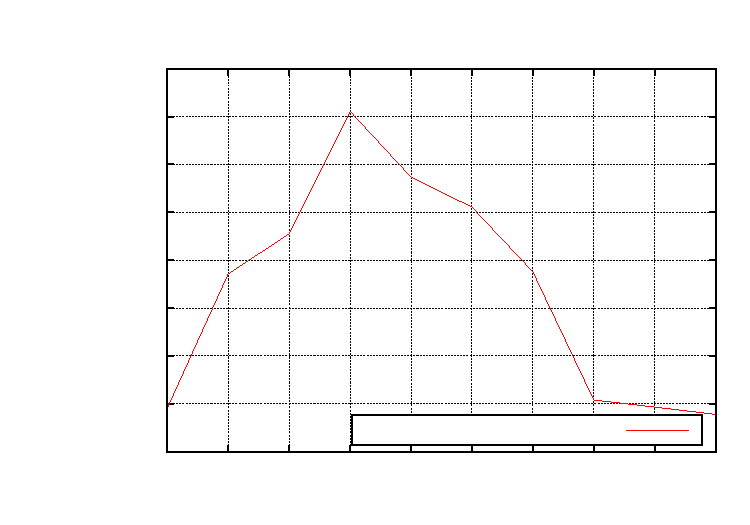
\includegraphics{diskgrowthrateh005}}%
    \gplfronttext
  \end{picture}%
\endgroup

	\end{center}
	\caption{Die Exzentrizitaet steigt am schnellsten bei q = 0.4 an. Die Growth Rate entspricht der linearen Steigung bei einem logarithmischen Plot der zeitlichen Entwicklung der Exzentrizitaet. Da aber alle Growth Rates sehr nahe beieinander sind und der lineare Teil Ermessenssache ist, sollte man diesen Plot mit Vorsicht betrachten!}
\end {figure}


\begin {figure}
	\begin{center}
		% GNUPLOT: LaTeX picture with Postscript
\begingroup
  \makeatletter
  \providecommand\color[2][]{%
    \GenericError{(gnuplot) \space\space\space\@spaces}{%
      Package color not loaded in conjunction with
      terminal option `colourtext'%
    }{See the gnuplot documentation for explanation.%
    }{Either use 'blacktext' in gnuplot or load the package
      color.sty in LaTeX.}%
    \renewcommand\color[2][]{}%
  }%
  \providecommand\includegraphics[2][]{%
    \GenericError{(gnuplot) \space\space\space\@spaces}{%
      Package graphicx or graphics not loaded%
    }{See the gnuplot documentation for explanation.%
    }{The gnuplot epslatex terminal needs graphicx.sty or graphics.sty.}%
    \renewcommand\includegraphics[2][]{}%
  }%
  \providecommand\rotatebox[2]{#2}%
  \@ifundefined{ifGPcolor}{%
    \newif\ifGPcolor
    \GPcolortrue
  }{}%
  \@ifundefined{ifGPblacktext}{%
    \newif\ifGPblacktext
    \GPblacktexttrue
  }{}%
  % define a \g@addto@macro without @ in the name:
  \let\gplgaddtomacro\g@addto@macro
  % define empty templates for all commands taking text:
  \gdef\gplbacktext{}%
  \gdef\gplfronttext{}%
  \makeatother
  \ifGPblacktext
    % no textcolor at all
    \def\colorrgb#1{}%
    \def\colorgray#1{}%
  \else
    % gray or color?
    \ifGPcolor
      \def\colorrgb#1{\color[rgb]{#1}}%
      \def\colorgray#1{\color[gray]{#1}}%
      \expandafter\def\csname LTw\endcsname{\color{white}}%
      \expandafter\def\csname LTb\endcsname{\color{black}}%
      \expandafter\def\csname LTa\endcsname{\color{black}}%
      \expandafter\def\csname LT0\endcsname{\color[rgb]{1,0,0}}%
      \expandafter\def\csname LT1\endcsname{\color[rgb]{0,1,0}}%
      \expandafter\def\csname LT2\endcsname{\color[rgb]{0,0,1}}%
      \expandafter\def\csname LT3\endcsname{\color[rgb]{1,0,1}}%
      \expandafter\def\csname LT4\endcsname{\color[rgb]{0,1,1}}%
      \expandafter\def\csname LT5\endcsname{\color[rgb]{1,1,0}}%
      \expandafter\def\csname LT6\endcsname{\color[rgb]{0,0,0}}%
      \expandafter\def\csname LT7\endcsname{\color[rgb]{1,0.3,0}}%
      \expandafter\def\csname LT8\endcsname{\color[rgb]{0.5,0.5,0.5}}%
    \else
      % gray
      \def\colorrgb#1{\color{black}}%
      \def\colorgray#1{\color[gray]{#1}}%
      \expandafter\def\csname LTw\endcsname{\color{white}}%
      \expandafter\def\csname LTb\endcsname{\color{black}}%
      \expandafter\def\csname LTa\endcsname{\color{black}}%
      \expandafter\def\csname LT0\endcsname{\color{black}}%
      \expandafter\def\csname LT1\endcsname{\color{black}}%
      \expandafter\def\csname LT2\endcsname{\color{black}}%
      \expandafter\def\csname LT3\endcsname{\color{black}}%
      \expandafter\def\csname LT4\endcsname{\color{black}}%
      \expandafter\def\csname LT5\endcsname{\color{black}}%
      \expandafter\def\csname LT6\endcsname{\color{black}}%
      \expandafter\def\csname LT7\endcsname{\color{black}}%
      \expandafter\def\csname LT8\endcsname{\color{black}}%
    \fi
  \fi
  \setlength{\unitlength}{0.0500bp}%
  \begin{picture}(8640.00,4032.00)%
    \gplgaddtomacro\gplbacktext{%
      \csname LTb\endcsname%
      \put(946,704){\makebox(0,0)[r]{\strut{}-4}}%
      \csname LTb\endcsname%
      \put(946,1085){\makebox(0,0)[r]{\strut{}-3}}%
      \csname LTb\endcsname%
      \put(946,1466){\makebox(0,0)[r]{\strut{}-2}}%
      \csname LTb\endcsname%
      \put(946,1847){\makebox(0,0)[r]{\strut{}-1}}%
      \csname LTb\endcsname%
      \put(946,2229){\makebox(0,0)[r]{\strut{} 0}}%
      \csname LTb\endcsname%
      \put(946,2610){\makebox(0,0)[r]{\strut{} 1}}%
      \csname LTb\endcsname%
      \put(946,2991){\makebox(0,0)[r]{\strut{} 2}}%
      \csname LTb\endcsname%
      \put(946,3372){\makebox(0,0)[r]{\strut{} 3}}%
      \csname LTb\endcsname%
      \put(1078,484){\makebox(0,0){\strut{} 0}}%
      \csname LTb\endcsname%
      \put(1982,484){\makebox(0,0){\strut{} 20}}%
      \csname LTb\endcsname%
      \put(2886,484){\makebox(0,0){\strut{} 40}}%
      \csname LTb\endcsname%
      \put(3790,484){\makebox(0,0){\strut{} 60}}%
      \csname LTb\endcsname%
      \put(4694,484){\makebox(0,0){\strut{} 80}}%
      \csname LTb\endcsname%
      \put(5598,484){\makebox(0,0){\strut{} 100}}%
      \csname LTb\endcsname%
      \put(6502,484){\makebox(0,0){\strut{} 120}}%
      \csname LTb\endcsname%
      \put(7406,484){\makebox(0,0){\strut{} 140}}%
      \csname LTb\endcsname%
      \put(8310,484){\makebox(0,0){\strut{} 160}}%
      \put(440,2038){\rotatebox{90}{\makebox(0,0){\strut{}Disk Periastron}}}%
      \put(4694,154){\makebox(0,0){\strut{}Time [$P_{\text{Orb}}$]}}%
      \put(4694,3702){\makebox(0,0){\strut{}h = 0.05}}%
    }%
    \gplgaddtomacro\gplfronttext{%
      \csname LTb\endcsname%
      \put(7323,910){\makebox(0,0)[r]{\strut{}q=0.1}}%
    }%
    \gplbacktext
    \put(0,0){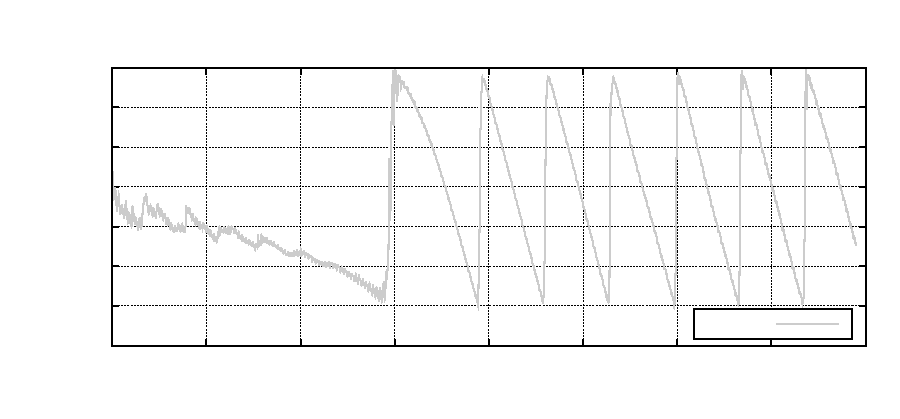
\includegraphics{diskperiastronh005q01}}%
    \gplfronttext
  \end{picture}%
\endgroup

	\end{center}
\end {figure}
\begin {figure}
	\begin{center}
		% GNUPLOT: LaTeX picture with Postscript
\begingroup
  \makeatletter
  \providecommand\color[2][]{%
    \GenericError{(gnuplot) \space\space\space\@spaces}{%
      Package color not loaded in conjunction with
      terminal option `colourtext'%
    }{See the gnuplot documentation for explanation.%
    }{Either use 'blacktext' in gnuplot or load the package
      color.sty in LaTeX.}%
    \renewcommand\color[2][]{}%
  }%
  \providecommand\includegraphics[2][]{%
    \GenericError{(gnuplot) \space\space\space\@spaces}{%
      Package graphicx or graphics not loaded%
    }{See the gnuplot documentation for explanation.%
    }{The gnuplot epslatex terminal needs graphicx.sty or graphics.sty.}%
    \renewcommand\includegraphics[2][]{}%
  }%
  \providecommand\rotatebox[2]{#2}%
  \@ifundefined{ifGPcolor}{%
    \newif\ifGPcolor
    \GPcolortrue
  }{}%
  \@ifundefined{ifGPblacktext}{%
    \newif\ifGPblacktext
    \GPblacktexttrue
  }{}%
  % define a \g@addto@macro without @ in the name:
  \let\gplgaddtomacro\g@addto@macro
  % define empty templates for all commands taking text:
  \gdef\gplbacktext{}%
  \gdef\gplfronttext{}%
  \makeatother
  \ifGPblacktext
    % no textcolor at all
    \def\colorrgb#1{}%
    \def\colorgray#1{}%
  \else
    % gray or color?
    \ifGPcolor
      \def\colorrgb#1{\color[rgb]{#1}}%
      \def\colorgray#1{\color[gray]{#1}}%
      \expandafter\def\csname LTw\endcsname{\color{white}}%
      \expandafter\def\csname LTb\endcsname{\color{black}}%
      \expandafter\def\csname LTa\endcsname{\color{black}}%
      \expandafter\def\csname LT0\endcsname{\color[rgb]{1,0,0}}%
      \expandafter\def\csname LT1\endcsname{\color[rgb]{0,1,0}}%
      \expandafter\def\csname LT2\endcsname{\color[rgb]{0,0,1}}%
      \expandafter\def\csname LT3\endcsname{\color[rgb]{1,0,1}}%
      \expandafter\def\csname LT4\endcsname{\color[rgb]{0,1,1}}%
      \expandafter\def\csname LT5\endcsname{\color[rgb]{1,1,0}}%
      \expandafter\def\csname LT6\endcsname{\color[rgb]{0,0,0}}%
      \expandafter\def\csname LT7\endcsname{\color[rgb]{1,0.3,0}}%
      \expandafter\def\csname LT8\endcsname{\color[rgb]{0.5,0.5,0.5}}%
    \else
      % gray
      \def\colorrgb#1{\color{black}}%
      \def\colorgray#1{\color[gray]{#1}}%
      \expandafter\def\csname LTw\endcsname{\color{white}}%
      \expandafter\def\csname LTb\endcsname{\color{black}}%
      \expandafter\def\csname LTa\endcsname{\color{black}}%
      \expandafter\def\csname LT0\endcsname{\color{black}}%
      \expandafter\def\csname LT1\endcsname{\color{black}}%
      \expandafter\def\csname LT2\endcsname{\color{black}}%
      \expandafter\def\csname LT3\endcsname{\color{black}}%
      \expandafter\def\csname LT4\endcsname{\color{black}}%
      \expandafter\def\csname LT5\endcsname{\color{black}}%
      \expandafter\def\csname LT6\endcsname{\color{black}}%
      \expandafter\def\csname LT7\endcsname{\color{black}}%
      \expandafter\def\csname LT8\endcsname{\color{black}}%
    \fi
  \fi
  \setlength{\unitlength}{0.0500bp}%
  \begin{picture}(8640.00,4032.00)%
    \gplgaddtomacro\gplbacktext{%
      \csname LTb\endcsname%
      \put(946,704){\makebox(0,0)[r]{\strut{}-4}}%
      \csname LTb\endcsname%
      \put(946,1085){\makebox(0,0)[r]{\strut{}-3}}%
      \csname LTb\endcsname%
      \put(946,1466){\makebox(0,0)[r]{\strut{}-2}}%
      \csname LTb\endcsname%
      \put(946,1847){\makebox(0,0)[r]{\strut{}-1}}%
      \csname LTb\endcsname%
      \put(946,2229){\makebox(0,0)[r]{\strut{} 0}}%
      \csname LTb\endcsname%
      \put(946,2610){\makebox(0,0)[r]{\strut{} 1}}%
      \csname LTb\endcsname%
      \put(946,2991){\makebox(0,0)[r]{\strut{} 2}}%
      \csname LTb\endcsname%
      \put(946,3372){\makebox(0,0)[r]{\strut{} 3}}%
      \csname LTb\endcsname%
      \put(1078,484){\makebox(0,0){\strut{} 0}}%
      \csname LTb\endcsname%
      \put(2283,484){\makebox(0,0){\strut{} 20}}%
      \csname LTb\endcsname%
      \put(3489,484){\makebox(0,0){\strut{} 40}}%
      \csname LTb\endcsname%
      \put(4694,484){\makebox(0,0){\strut{} 60}}%
      \csname LTb\endcsname%
      \put(5899,484){\makebox(0,0){\strut{} 80}}%
      \csname LTb\endcsname%
      \put(7105,484){\makebox(0,0){\strut{} 100}}%
      \csname LTb\endcsname%
      \put(8310,484){\makebox(0,0){\strut{} 120}}%
      \put(440,2038){\rotatebox{90}{\makebox(0,0){\strut{}Disk Periastron}}}%
      \put(4694,154){\makebox(0,0){\strut{}Time [$P_{\text{Orb}}$]}}%
      \put(4694,3702){\makebox(0,0){\strut{}h = 0.05}}%
    }%
    \gplgaddtomacro\gplfronttext{%
      \csname LTb\endcsname%
      \put(7323,910){\makebox(0,0)[r]{\strut{}q=0.2}}%
    }%
    \gplbacktext
    \put(0,0){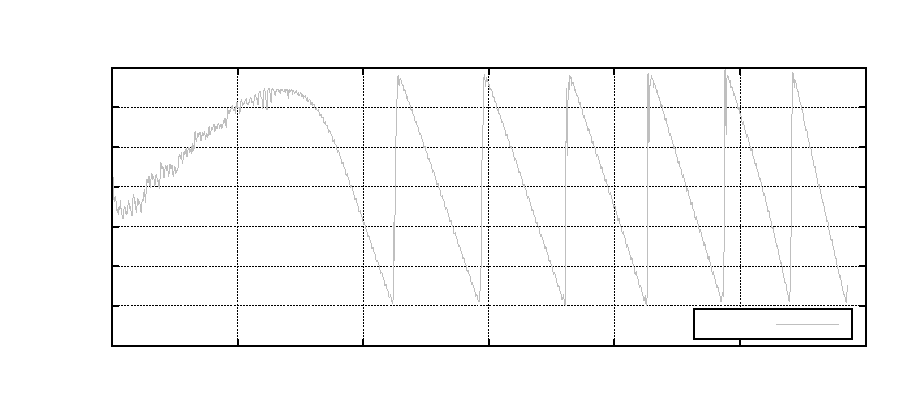
\includegraphics{diskperiastronh005q02}}%
    \gplfronttext
  \end{picture}%
\endgroup

	\end{center}
\end {figure}
\begin {figure}
	\begin{center}
		% GNUPLOT: LaTeX picture with Postscript
\begingroup
  \makeatletter
  \providecommand\color[2][]{%
    \GenericError{(gnuplot) \space\space\space\@spaces}{%
      Package color not loaded in conjunction with
      terminal option `colourtext'%
    }{See the gnuplot documentation for explanation.%
    }{Either use 'blacktext' in gnuplot or load the package
      color.sty in LaTeX.}%
    \renewcommand\color[2][]{}%
  }%
  \providecommand\includegraphics[2][]{%
    \GenericError{(gnuplot) \space\space\space\@spaces}{%
      Package graphicx or graphics not loaded%
    }{See the gnuplot documentation for explanation.%
    }{The gnuplot epslatex terminal needs graphicx.sty or graphics.sty.}%
    \renewcommand\includegraphics[2][]{}%
  }%
  \providecommand\rotatebox[2]{#2}%
  \@ifundefined{ifGPcolor}{%
    \newif\ifGPcolor
    \GPcolortrue
  }{}%
  \@ifundefined{ifGPblacktext}{%
    \newif\ifGPblacktext
    \GPblacktexttrue
  }{}%
  % define a \g@addto@macro without @ in the name:
  \let\gplgaddtomacro\g@addto@macro
  % define empty templates for all commands taking text:
  \gdef\gplbacktext{}%
  \gdef\gplfronttext{}%
  \makeatother
  \ifGPblacktext
    % no textcolor at all
    \def\colorrgb#1{}%
    \def\colorgray#1{}%
  \else
    % gray or color?
    \ifGPcolor
      \def\colorrgb#1{\color[rgb]{#1}}%
      \def\colorgray#1{\color[gray]{#1}}%
      \expandafter\def\csname LTw\endcsname{\color{white}}%
      \expandafter\def\csname LTb\endcsname{\color{black}}%
      \expandafter\def\csname LTa\endcsname{\color{black}}%
      \expandafter\def\csname LT0\endcsname{\color[rgb]{1,0,0}}%
      \expandafter\def\csname LT1\endcsname{\color[rgb]{0,1,0}}%
      \expandafter\def\csname LT2\endcsname{\color[rgb]{0,0,1}}%
      \expandafter\def\csname LT3\endcsname{\color[rgb]{1,0,1}}%
      \expandafter\def\csname LT4\endcsname{\color[rgb]{0,1,1}}%
      \expandafter\def\csname LT5\endcsname{\color[rgb]{1,1,0}}%
      \expandafter\def\csname LT6\endcsname{\color[rgb]{0,0,0}}%
      \expandafter\def\csname LT7\endcsname{\color[rgb]{1,0.3,0}}%
      \expandafter\def\csname LT8\endcsname{\color[rgb]{0.5,0.5,0.5}}%
    \else
      % gray
      \def\colorrgb#1{\color{black}}%
      \def\colorgray#1{\color[gray]{#1}}%
      \expandafter\def\csname LTw\endcsname{\color{white}}%
      \expandafter\def\csname LTb\endcsname{\color{black}}%
      \expandafter\def\csname LTa\endcsname{\color{black}}%
      \expandafter\def\csname LT0\endcsname{\color{black}}%
      \expandafter\def\csname LT1\endcsname{\color{black}}%
      \expandafter\def\csname LT2\endcsname{\color{black}}%
      \expandafter\def\csname LT3\endcsname{\color{black}}%
      \expandafter\def\csname LT4\endcsname{\color{black}}%
      \expandafter\def\csname LT5\endcsname{\color{black}}%
      \expandafter\def\csname LT6\endcsname{\color{black}}%
      \expandafter\def\csname LT7\endcsname{\color{black}}%
      \expandafter\def\csname LT8\endcsname{\color{black}}%
    \fi
  \fi
  \setlength{\unitlength}{0.0500bp}%
  \begin{picture}(8640.00,4032.00)%
    \gplgaddtomacro\gplbacktext{%
      \csname LTb\endcsname%
      \put(946,704){\makebox(0,0)[r]{\strut{}-4}}%
      \csname LTb\endcsname%
      \put(946,1085){\makebox(0,0)[r]{\strut{}-3}}%
      \csname LTb\endcsname%
      \put(946,1466){\makebox(0,0)[r]{\strut{}-2}}%
      \csname LTb\endcsname%
      \put(946,1847){\makebox(0,0)[r]{\strut{}-1}}%
      \csname LTb\endcsname%
      \put(946,2229){\makebox(0,0)[r]{\strut{} 0}}%
      \csname LTb\endcsname%
      \put(946,2610){\makebox(0,0)[r]{\strut{} 1}}%
      \csname LTb\endcsname%
      \put(946,2991){\makebox(0,0)[r]{\strut{} 2}}%
      \csname LTb\endcsname%
      \put(946,3372){\makebox(0,0)[r]{\strut{} 3}}%
      \csname LTb\endcsname%
      \put(1078,484){\makebox(0,0){\strut{} 0}}%
      \csname LTb\endcsname%
      \put(1801,484){\makebox(0,0){\strut{} 10}}%
      \csname LTb\endcsname%
      \put(2524,484){\makebox(0,0){\strut{} 20}}%
      \csname LTb\endcsname%
      \put(3248,484){\makebox(0,0){\strut{} 30}}%
      \csname LTb\endcsname%
      \put(3971,484){\makebox(0,0){\strut{} 40}}%
      \csname LTb\endcsname%
      \put(4694,484){\makebox(0,0){\strut{} 50}}%
      \csname LTb\endcsname%
      \put(5417,484){\makebox(0,0){\strut{} 60}}%
      \csname LTb\endcsname%
      \put(6140,484){\makebox(0,0){\strut{} 70}}%
      \csname LTb\endcsname%
      \put(6864,484){\makebox(0,0){\strut{} 80}}%
      \csname LTb\endcsname%
      \put(7587,484){\makebox(0,0){\strut{} 90}}%
      \csname LTb\endcsname%
      \put(8310,484){\makebox(0,0){\strut{} 100}}%
      \put(440,2038){\rotatebox{90}{\makebox(0,0){\strut{}Disk Periastron}}}%
      \put(4694,154){\makebox(0,0){\strut{}Time [$P_{\text{Orb}}$]}}%
      \put(4694,3702){\makebox(0,0){\strut{}h = 0.05}}%
    }%
    \gplgaddtomacro\gplfronttext{%
      \csname LTb\endcsname%
      \put(7323,910){\makebox(0,0)[r]{\strut{}q=0.3}}%
    }%
    \gplbacktext
    \put(0,0){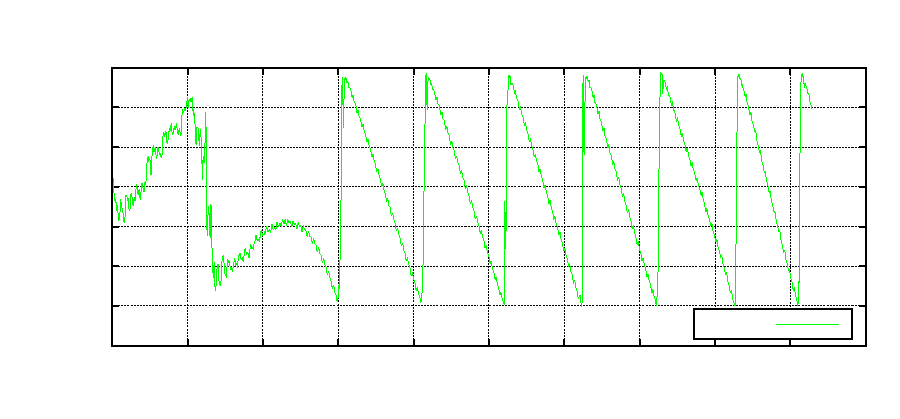
\includegraphics{diskperiastronh005q03}}%
    \gplfronttext
  \end{picture}%
\endgroup

	\end{center}
\end {figure}
\begin {figure}
	\begin{center}
		% GNUPLOT: LaTeX picture with Postscript
\begingroup
  \makeatletter
  \providecommand\color[2][]{%
    \GenericError{(gnuplot) \space\space\space\@spaces}{%
      Package color not loaded in conjunction with
      terminal option `colourtext'%
    }{See the gnuplot documentation for explanation.%
    }{Either use 'blacktext' in gnuplot or load the package
      color.sty in LaTeX.}%
    \renewcommand\color[2][]{}%
  }%
  \providecommand\includegraphics[2][]{%
    \GenericError{(gnuplot) \space\space\space\@spaces}{%
      Package graphicx or graphics not loaded%
    }{See the gnuplot documentation for explanation.%
    }{The gnuplot epslatex terminal needs graphicx.sty or graphics.sty.}%
    \renewcommand\includegraphics[2][]{}%
  }%
  \providecommand\rotatebox[2]{#2}%
  \@ifundefined{ifGPcolor}{%
    \newif\ifGPcolor
    \GPcolortrue
  }{}%
  \@ifundefined{ifGPblacktext}{%
    \newif\ifGPblacktext
    \GPblacktexttrue
  }{}%
  % define a \g@addto@macro without @ in the name:
  \let\gplgaddtomacro\g@addto@macro
  % define empty templates for all commands taking text:
  \gdef\gplbacktext{}%
  \gdef\gplfronttext{}%
  \makeatother
  \ifGPblacktext
    % no textcolor at all
    \def\colorrgb#1{}%
    \def\colorgray#1{}%
  \else
    % gray or color?
    \ifGPcolor
      \def\colorrgb#1{\color[rgb]{#1}}%
      \def\colorgray#1{\color[gray]{#1}}%
      \expandafter\def\csname LTw\endcsname{\color{white}}%
      \expandafter\def\csname LTb\endcsname{\color{black}}%
      \expandafter\def\csname LTa\endcsname{\color{black}}%
      \expandafter\def\csname LT0\endcsname{\color[rgb]{1,0,0}}%
      \expandafter\def\csname LT1\endcsname{\color[rgb]{0,1,0}}%
      \expandafter\def\csname LT2\endcsname{\color[rgb]{0,0,1}}%
      \expandafter\def\csname LT3\endcsname{\color[rgb]{1,0,1}}%
      \expandafter\def\csname LT4\endcsname{\color[rgb]{0,1,1}}%
      \expandafter\def\csname LT5\endcsname{\color[rgb]{1,1,0}}%
      \expandafter\def\csname LT6\endcsname{\color[rgb]{0,0,0}}%
      \expandafter\def\csname LT7\endcsname{\color[rgb]{1,0.3,0}}%
      \expandafter\def\csname LT8\endcsname{\color[rgb]{0.5,0.5,0.5}}%
    \else
      % gray
      \def\colorrgb#1{\color{black}}%
      \def\colorgray#1{\color[gray]{#1}}%
      \expandafter\def\csname LTw\endcsname{\color{white}}%
      \expandafter\def\csname LTb\endcsname{\color{black}}%
      \expandafter\def\csname LTa\endcsname{\color{black}}%
      \expandafter\def\csname LT0\endcsname{\color{black}}%
      \expandafter\def\csname LT1\endcsname{\color{black}}%
      \expandafter\def\csname LT2\endcsname{\color{black}}%
      \expandafter\def\csname LT3\endcsname{\color{black}}%
      \expandafter\def\csname LT4\endcsname{\color{black}}%
      \expandafter\def\csname LT5\endcsname{\color{black}}%
      \expandafter\def\csname LT6\endcsname{\color{black}}%
      \expandafter\def\csname LT7\endcsname{\color{black}}%
      \expandafter\def\csname LT8\endcsname{\color{black}}%
    \fi
  \fi
  \setlength{\unitlength}{0.0500bp}%
  \begin{picture}(8640.00,4032.00)%
    \gplgaddtomacro\gplbacktext{%
      \csname LTb\endcsname%
      \put(946,704){\makebox(0,0)[r]{\strut{}-4}}%
      \csname LTb\endcsname%
      \put(946,1085){\makebox(0,0)[r]{\strut{}-3}}%
      \csname LTb\endcsname%
      \put(946,1466){\makebox(0,0)[r]{\strut{}-2}}%
      \csname LTb\endcsname%
      \put(946,1847){\makebox(0,0)[r]{\strut{}-1}}%
      \csname LTb\endcsname%
      \put(946,2229){\makebox(0,0)[r]{\strut{} 0}}%
      \csname LTb\endcsname%
      \put(946,2610){\makebox(0,0)[r]{\strut{} 1}}%
      \csname LTb\endcsname%
      \put(946,2991){\makebox(0,0)[r]{\strut{} 2}}%
      \csname LTb\endcsname%
      \put(946,3372){\makebox(0,0)[r]{\strut{} 3}}%
      \csname LTb\endcsname%
      \put(1078,484){\makebox(0,0){\strut{} 0}}%
      \csname LTb\endcsname%
      \put(2111,484){\makebox(0,0){\strut{} 20}}%
      \csname LTb\endcsname%
      \put(3144,484){\makebox(0,0){\strut{} 40}}%
      \csname LTb\endcsname%
      \put(4177,484){\makebox(0,0){\strut{} 60}}%
      \csname LTb\endcsname%
      \put(5211,484){\makebox(0,0){\strut{} 80}}%
      \csname LTb\endcsname%
      \put(6244,484){\makebox(0,0){\strut{} 100}}%
      \csname LTb\endcsname%
      \put(7277,484){\makebox(0,0){\strut{} 120}}%
      \csname LTb\endcsname%
      \put(8310,484){\makebox(0,0){\strut{} 140}}%
      \put(440,2038){\rotatebox{90}{\makebox(0,0){\strut{}Disk Periastron}}}%
      \put(4694,154){\makebox(0,0){\strut{}Time [$P_{\text{Orb}}$]}}%
      \put(4694,3702){\makebox(0,0){\strut{}h = 0.05}}%
    }%
    \gplgaddtomacro\gplfronttext{%
      \csname LTb\endcsname%
      \put(7323,910){\makebox(0,0)[r]{\strut{}q=0.4}}%
    }%
    \gplbacktext
    \put(0,0){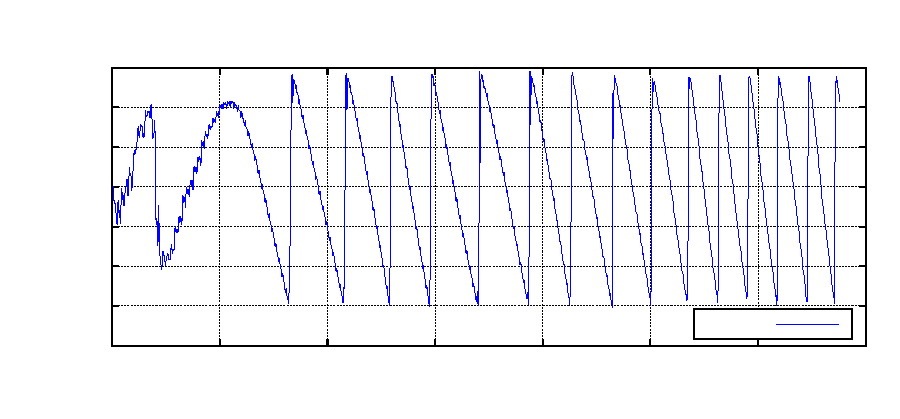
\includegraphics{diskperiastronh005q04}}%
    \gplfronttext
  \end{picture}%
\endgroup

	\end{center}
\end {figure}
\begin {figure}
	\begin{center}
		% GNUPLOT: LaTeX picture with Postscript
\begingroup
  \makeatletter
  \providecommand\color[2][]{%
    \GenericError{(gnuplot) \space\space\space\@spaces}{%
      Package color not loaded in conjunction with
      terminal option `colourtext'%
    }{See the gnuplot documentation for explanation.%
    }{Either use 'blacktext' in gnuplot or load the package
      color.sty in LaTeX.}%
    \renewcommand\color[2][]{}%
  }%
  \providecommand\includegraphics[2][]{%
    \GenericError{(gnuplot) \space\space\space\@spaces}{%
      Package graphicx or graphics not loaded%
    }{See the gnuplot documentation for explanation.%
    }{The gnuplot epslatex terminal needs graphicx.sty or graphics.sty.}%
    \renewcommand\includegraphics[2][]{}%
  }%
  \providecommand\rotatebox[2]{#2}%
  \@ifundefined{ifGPcolor}{%
    \newif\ifGPcolor
    \GPcolortrue
  }{}%
  \@ifundefined{ifGPblacktext}{%
    \newif\ifGPblacktext
    \GPblacktexttrue
  }{}%
  % define a \g@addto@macro without @ in the name:
  \let\gplgaddtomacro\g@addto@macro
  % define empty templates for all commands taking text:
  \gdef\gplbacktext{}%
  \gdef\gplfronttext{}%
  \makeatother
  \ifGPblacktext
    % no textcolor at all
    \def\colorrgb#1{}%
    \def\colorgray#1{}%
  \else
    % gray or color?
    \ifGPcolor
      \def\colorrgb#1{\color[rgb]{#1}}%
      \def\colorgray#1{\color[gray]{#1}}%
      \expandafter\def\csname LTw\endcsname{\color{white}}%
      \expandafter\def\csname LTb\endcsname{\color{black}}%
      \expandafter\def\csname LTa\endcsname{\color{black}}%
      \expandafter\def\csname LT0\endcsname{\color[rgb]{1,0,0}}%
      \expandafter\def\csname LT1\endcsname{\color[rgb]{0,1,0}}%
      \expandafter\def\csname LT2\endcsname{\color[rgb]{0,0,1}}%
      \expandafter\def\csname LT3\endcsname{\color[rgb]{1,0,1}}%
      \expandafter\def\csname LT4\endcsname{\color[rgb]{0,1,1}}%
      \expandafter\def\csname LT5\endcsname{\color[rgb]{1,1,0}}%
      \expandafter\def\csname LT6\endcsname{\color[rgb]{0,0,0}}%
      \expandafter\def\csname LT7\endcsname{\color[rgb]{1,0.3,0}}%
      \expandafter\def\csname LT8\endcsname{\color[rgb]{0.5,0.5,0.5}}%
    \else
      % gray
      \def\colorrgb#1{\color{black}}%
      \def\colorgray#1{\color[gray]{#1}}%
      \expandafter\def\csname LTw\endcsname{\color{white}}%
      \expandafter\def\csname LTb\endcsname{\color{black}}%
      \expandafter\def\csname LTa\endcsname{\color{black}}%
      \expandafter\def\csname LT0\endcsname{\color{black}}%
      \expandafter\def\csname LT1\endcsname{\color{black}}%
      \expandafter\def\csname LT2\endcsname{\color{black}}%
      \expandafter\def\csname LT3\endcsname{\color{black}}%
      \expandafter\def\csname LT4\endcsname{\color{black}}%
      \expandafter\def\csname LT5\endcsname{\color{black}}%
      \expandafter\def\csname LT6\endcsname{\color{black}}%
      \expandafter\def\csname LT7\endcsname{\color{black}}%
      \expandafter\def\csname LT8\endcsname{\color{black}}%
    \fi
  \fi
  \setlength{\unitlength}{0.0500bp}%
  \begin{picture}(8640.00,4032.00)%
    \gplgaddtomacro\gplbacktext{%
      \csname LTb\endcsname%
      \put(946,704){\makebox(0,0)[r]{\strut{}-4}}%
      \csname LTb\endcsname%
      \put(946,1085){\makebox(0,0)[r]{\strut{}-3}}%
      \csname LTb\endcsname%
      \put(946,1466){\makebox(0,0)[r]{\strut{}-2}}%
      \csname LTb\endcsname%
      \put(946,1847){\makebox(0,0)[r]{\strut{}-1}}%
      \csname LTb\endcsname%
      \put(946,2229){\makebox(0,0)[r]{\strut{} 0}}%
      \csname LTb\endcsname%
      \put(946,2610){\makebox(0,0)[r]{\strut{} 1}}%
      \csname LTb\endcsname%
      \put(946,2991){\makebox(0,0)[r]{\strut{} 2}}%
      \csname LTb\endcsname%
      \put(946,3372){\makebox(0,0)[r]{\strut{} 3}}%
      \csname LTb\endcsname%
      \put(1078,484){\makebox(0,0){\strut{} 0}}%
      \csname LTb\endcsname%
      \put(2111,484){\makebox(0,0){\strut{} 20}}%
      \csname LTb\endcsname%
      \put(3144,484){\makebox(0,0){\strut{} 40}}%
      \csname LTb\endcsname%
      \put(4177,484){\makebox(0,0){\strut{} 60}}%
      \csname LTb\endcsname%
      \put(5211,484){\makebox(0,0){\strut{} 80}}%
      \csname LTb\endcsname%
      \put(6244,484){\makebox(0,0){\strut{} 100}}%
      \csname LTb\endcsname%
      \put(7277,484){\makebox(0,0){\strut{} 120}}%
      \csname LTb\endcsname%
      \put(8310,484){\makebox(0,0){\strut{} 140}}%
      \put(440,2038){\rotatebox{90}{\makebox(0,0){\strut{}Disk Periastron}}}%
      \put(4694,154){\makebox(0,0){\strut{}Time [$P_{\text{Orb}}$]}}%
      \put(4694,3702){\makebox(0,0){\strut{}h = 0.05}}%
    }%
    \gplgaddtomacro\gplfronttext{%
      \csname LTb\endcsname%
      \put(7323,910){\makebox(0,0)[r]{\strut{}q=0.5}}%
    }%
    \gplbacktext
    \put(0,0){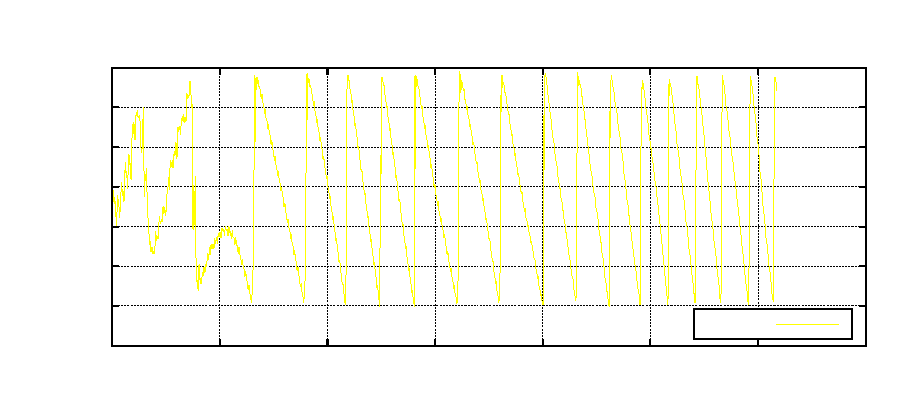
\includegraphics{diskperiastronh005q05}}%
    \gplfronttext
  \end{picture}%
\endgroup

	\end{center}
\end {figure}
\begin {figure}
	\begin{center}
		% GNUPLOT: LaTeX picture with Postscript
\begingroup
  \makeatletter
  \providecommand\color[2][]{%
    \GenericError{(gnuplot) \space\space\space\@spaces}{%
      Package color not loaded in conjunction with
      terminal option `colourtext'%
    }{See the gnuplot documentation for explanation.%
    }{Either use 'blacktext' in gnuplot or load the package
      color.sty in LaTeX.}%
    \renewcommand\color[2][]{}%
  }%
  \providecommand\includegraphics[2][]{%
    \GenericError{(gnuplot) \space\space\space\@spaces}{%
      Package graphicx or graphics not loaded%
    }{See the gnuplot documentation for explanation.%
    }{The gnuplot epslatex terminal needs graphicx.sty or graphics.sty.}%
    \renewcommand\includegraphics[2][]{}%
  }%
  \providecommand\rotatebox[2]{#2}%
  \@ifundefined{ifGPcolor}{%
    \newif\ifGPcolor
    \GPcolortrue
  }{}%
  \@ifundefined{ifGPblacktext}{%
    \newif\ifGPblacktext
    \GPblacktexttrue
  }{}%
  % define a \g@addto@macro without @ in the name:
  \let\gplgaddtomacro\g@addto@macro
  % define empty templates for all commands taking text:
  \gdef\gplbacktext{}%
  \gdef\gplfronttext{}%
  \makeatother
  \ifGPblacktext
    % no textcolor at all
    \def\colorrgb#1{}%
    \def\colorgray#1{}%
  \else
    % gray or color?
    \ifGPcolor
      \def\colorrgb#1{\color[rgb]{#1}}%
      \def\colorgray#1{\color[gray]{#1}}%
      \expandafter\def\csname LTw\endcsname{\color{white}}%
      \expandafter\def\csname LTb\endcsname{\color{black}}%
      \expandafter\def\csname LTa\endcsname{\color{black}}%
      \expandafter\def\csname LT0\endcsname{\color[rgb]{1,0,0}}%
      \expandafter\def\csname LT1\endcsname{\color[rgb]{0,1,0}}%
      \expandafter\def\csname LT2\endcsname{\color[rgb]{0,0,1}}%
      \expandafter\def\csname LT3\endcsname{\color[rgb]{1,0,1}}%
      \expandafter\def\csname LT4\endcsname{\color[rgb]{0,1,1}}%
      \expandafter\def\csname LT5\endcsname{\color[rgb]{1,1,0}}%
      \expandafter\def\csname LT6\endcsname{\color[rgb]{0,0,0}}%
      \expandafter\def\csname LT7\endcsname{\color[rgb]{1,0.3,0}}%
      \expandafter\def\csname LT8\endcsname{\color[rgb]{0.5,0.5,0.5}}%
    \else
      % gray
      \def\colorrgb#1{\color{black}}%
      \def\colorgray#1{\color[gray]{#1}}%
      \expandafter\def\csname LTw\endcsname{\color{white}}%
      \expandafter\def\csname LTb\endcsname{\color{black}}%
      \expandafter\def\csname LTa\endcsname{\color{black}}%
      \expandafter\def\csname LT0\endcsname{\color{black}}%
      \expandafter\def\csname LT1\endcsname{\color{black}}%
      \expandafter\def\csname LT2\endcsname{\color{black}}%
      \expandafter\def\csname LT3\endcsname{\color{black}}%
      \expandafter\def\csname LT4\endcsname{\color{black}}%
      \expandafter\def\csname LT5\endcsname{\color{black}}%
      \expandafter\def\csname LT6\endcsname{\color{black}}%
      \expandafter\def\csname LT7\endcsname{\color{black}}%
      \expandafter\def\csname LT8\endcsname{\color{black}}%
    \fi
  \fi
  \setlength{\unitlength}{0.0500bp}%
  \begin{picture}(8640.00,4032.00)%
    \gplgaddtomacro\gplbacktext{%
      \csname LTb\endcsname%
      \put(946,704){\makebox(0,0)[r]{\strut{}-4}}%
      \csname LTb\endcsname%
      \put(946,1085){\makebox(0,0)[r]{\strut{}-3}}%
      \csname LTb\endcsname%
      \put(946,1466){\makebox(0,0)[r]{\strut{}-2}}%
      \csname LTb\endcsname%
      \put(946,1847){\makebox(0,0)[r]{\strut{}-1}}%
      \csname LTb\endcsname%
      \put(946,2229){\makebox(0,0)[r]{\strut{} 0}}%
      \csname LTb\endcsname%
      \put(946,2610){\makebox(0,0)[r]{\strut{} 1}}%
      \csname LTb\endcsname%
      \put(946,2991){\makebox(0,0)[r]{\strut{} 2}}%
      \csname LTb\endcsname%
      \put(946,3372){\makebox(0,0)[r]{\strut{} 3}}%
      \csname LTb\endcsname%
      \put(1078,484){\makebox(0,0){\strut{} 0}}%
      \csname LTb\endcsname%
      \put(2111,484){\makebox(0,0){\strut{} 10}}%
      \csname LTb\endcsname%
      \put(3144,484){\makebox(0,0){\strut{} 20}}%
      \csname LTb\endcsname%
      \put(4177,484){\makebox(0,0){\strut{} 30}}%
      \csname LTb\endcsname%
      \put(5211,484){\makebox(0,0){\strut{} 40}}%
      \csname LTb\endcsname%
      \put(6244,484){\makebox(0,0){\strut{} 50}}%
      \csname LTb\endcsname%
      \put(7277,484){\makebox(0,0){\strut{} 60}}%
      \csname LTb\endcsname%
      \put(8310,484){\makebox(0,0){\strut{} 70}}%
      \put(440,2038){\rotatebox{90}{\makebox(0,0){\strut{}Disk Periastron}}}%
      \put(4694,154){\makebox(0,0){\strut{}Time [$P_{\text{Orb}}$]}}%
      \put(4694,3702){\makebox(0,0){\strut{}h = 0.05}}%
    }%
    \gplgaddtomacro\gplfronttext{%
      \csname LTb\endcsname%
      \put(7323,910){\makebox(0,0)[r]{\strut{}q=0.6}}%
    }%
    \gplbacktext
    \put(0,0){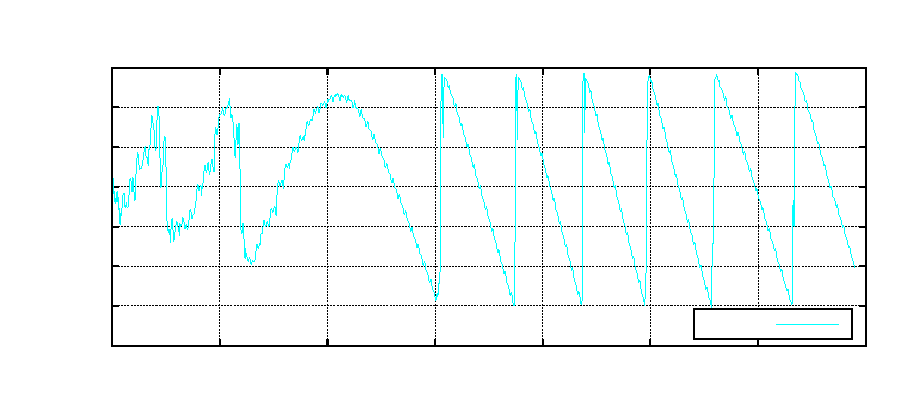
\includegraphics{diskperiastronh005q06}}%
    \gplfronttext
  \end{picture}%
\endgroup

	\end{center}
\end {figure}
\begin {figure}
	\begin{center}
		% GNUPLOT: LaTeX picture with Postscript
\begingroup
  \makeatletter
  \providecommand\color[2][]{%
    \GenericError{(gnuplot) \space\space\space\@spaces}{%
      Package color not loaded in conjunction with
      terminal option `colourtext'%
    }{See the gnuplot documentation for explanation.%
    }{Either use 'blacktext' in gnuplot or load the package
      color.sty in LaTeX.}%
    \renewcommand\color[2][]{}%
  }%
  \providecommand\includegraphics[2][]{%
    \GenericError{(gnuplot) \space\space\space\@spaces}{%
      Package graphicx or graphics not loaded%
    }{See the gnuplot documentation for explanation.%
    }{The gnuplot epslatex terminal needs graphicx.sty or graphics.sty.}%
    \renewcommand\includegraphics[2][]{}%
  }%
  \providecommand\rotatebox[2]{#2}%
  \@ifundefined{ifGPcolor}{%
    \newif\ifGPcolor
    \GPcolortrue
  }{}%
  \@ifundefined{ifGPblacktext}{%
    \newif\ifGPblacktext
    \GPblacktexttrue
  }{}%
  % define a \g@addto@macro without @ in the name:
  \let\gplgaddtomacro\g@addto@macro
  % define empty templates for all commands taking text:
  \gdef\gplbacktext{}%
  \gdef\gplfronttext{}%
  \makeatother
  \ifGPblacktext
    % no textcolor at all
    \def\colorrgb#1{}%
    \def\colorgray#1{}%
  \else
    % gray or color?
    \ifGPcolor
      \def\colorrgb#1{\color[rgb]{#1}}%
      \def\colorgray#1{\color[gray]{#1}}%
      \expandafter\def\csname LTw\endcsname{\color{white}}%
      \expandafter\def\csname LTb\endcsname{\color{black}}%
      \expandafter\def\csname LTa\endcsname{\color{black}}%
      \expandafter\def\csname LT0\endcsname{\color[rgb]{1,0,0}}%
      \expandafter\def\csname LT1\endcsname{\color[rgb]{0,1,0}}%
      \expandafter\def\csname LT2\endcsname{\color[rgb]{0,0,1}}%
      \expandafter\def\csname LT3\endcsname{\color[rgb]{1,0,1}}%
      \expandafter\def\csname LT4\endcsname{\color[rgb]{0,1,1}}%
      \expandafter\def\csname LT5\endcsname{\color[rgb]{1,1,0}}%
      \expandafter\def\csname LT6\endcsname{\color[rgb]{0,0,0}}%
      \expandafter\def\csname LT7\endcsname{\color[rgb]{1,0.3,0}}%
      \expandafter\def\csname LT8\endcsname{\color[rgb]{0.5,0.5,0.5}}%
    \else
      % gray
      \def\colorrgb#1{\color{black}}%
      \def\colorgray#1{\color[gray]{#1}}%
      \expandafter\def\csname LTw\endcsname{\color{white}}%
      \expandafter\def\csname LTb\endcsname{\color{black}}%
      \expandafter\def\csname LTa\endcsname{\color{black}}%
      \expandafter\def\csname LT0\endcsname{\color{black}}%
      \expandafter\def\csname LT1\endcsname{\color{black}}%
      \expandafter\def\csname LT2\endcsname{\color{black}}%
      \expandafter\def\csname LT3\endcsname{\color{black}}%
      \expandafter\def\csname LT4\endcsname{\color{black}}%
      \expandafter\def\csname LT5\endcsname{\color{black}}%
      \expandafter\def\csname LT6\endcsname{\color{black}}%
      \expandafter\def\csname LT7\endcsname{\color{black}}%
      \expandafter\def\csname LT8\endcsname{\color{black}}%
    \fi
  \fi
  \setlength{\unitlength}{0.0500bp}%
  \begin{picture}(8640.00,4032.00)%
    \gplgaddtomacro\gplbacktext{%
      \csname LTb\endcsname%
      \put(946,704){\makebox(0,0)[r]{\strut{}-4}}%
      \csname LTb\endcsname%
      \put(946,1085){\makebox(0,0)[r]{\strut{}-3}}%
      \csname LTb\endcsname%
      \put(946,1466){\makebox(0,0)[r]{\strut{}-2}}%
      \csname LTb\endcsname%
      \put(946,1847){\makebox(0,0)[r]{\strut{}-1}}%
      \csname LTb\endcsname%
      \put(946,2229){\makebox(0,0)[r]{\strut{} 0}}%
      \csname LTb\endcsname%
      \put(946,2610){\makebox(0,0)[r]{\strut{} 1}}%
      \csname LTb\endcsname%
      \put(946,2991){\makebox(0,0)[r]{\strut{} 2}}%
      \csname LTb\endcsname%
      \put(946,3372){\makebox(0,0)[r]{\strut{} 3}}%
      \csname LTb\endcsname%
      \put(1078,484){\makebox(0,0){\strut{} 0}}%
      \csname LTb\endcsname%
      \put(2283,484){\makebox(0,0){\strut{} 20}}%
      \csname LTb\endcsname%
      \put(3489,484){\makebox(0,0){\strut{} 40}}%
      \csname LTb\endcsname%
      \put(4694,484){\makebox(0,0){\strut{} 60}}%
      \csname LTb\endcsname%
      \put(5899,484){\makebox(0,0){\strut{} 80}}%
      \csname LTb\endcsname%
      \put(7105,484){\makebox(0,0){\strut{} 100}}%
      \csname LTb\endcsname%
      \put(8310,484){\makebox(0,0){\strut{} 120}}%
      \put(440,2038){\rotatebox{90}{\makebox(0,0){\strut{}Disk Periastron}}}%
      \put(4694,154){\makebox(0,0){\strut{}Time [$P_{\text{Orb}}$]}}%
      \put(4694,3702){\makebox(0,0){\strut{}h = 0.05}}%
    }%
    \gplgaddtomacro\gplfronttext{%
      \csname LTb\endcsname%
      \put(7323,910){\makebox(0,0)[r]{\strut{}q=0.7}}%
    }%
    \gplbacktext
    \put(0,0){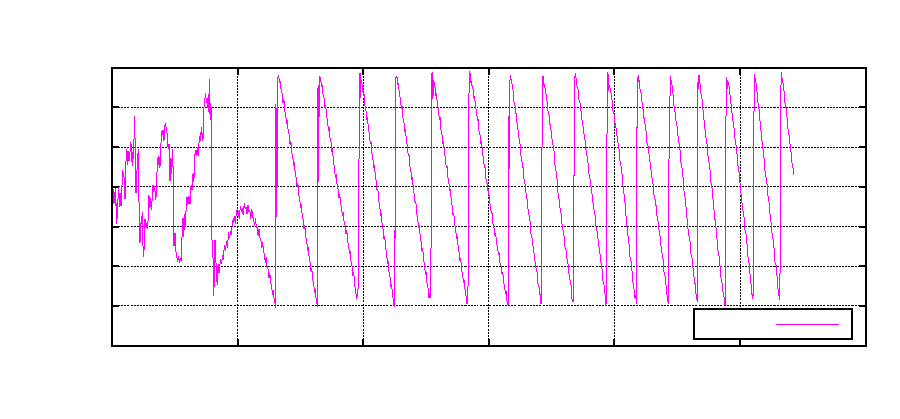
\includegraphics{diskperiastronh005q07}}%
    \gplfronttext
  \end{picture}%
\endgroup

	\end{center}
\end {figure}
\begin {figure}
	\begin{center}
		% GNUPLOT: LaTeX picture with Postscript
\begingroup
  \makeatletter
  \providecommand\color[2][]{%
    \GenericError{(gnuplot) \space\space\space\@spaces}{%
      Package color not loaded in conjunction with
      terminal option `colourtext'%
    }{See the gnuplot documentation for explanation.%
    }{Either use 'blacktext' in gnuplot or load the package
      color.sty in LaTeX.}%
    \renewcommand\color[2][]{}%
  }%
  \providecommand\includegraphics[2][]{%
    \GenericError{(gnuplot) \space\space\space\@spaces}{%
      Package graphicx or graphics not loaded%
    }{See the gnuplot documentation for explanation.%
    }{The gnuplot epslatex terminal needs graphicx.sty or graphics.sty.}%
    \renewcommand\includegraphics[2][]{}%
  }%
  \providecommand\rotatebox[2]{#2}%
  \@ifundefined{ifGPcolor}{%
    \newif\ifGPcolor
    \GPcolortrue
  }{}%
  \@ifundefined{ifGPblacktext}{%
    \newif\ifGPblacktext
    \GPblacktexttrue
  }{}%
  % define a \g@addto@macro without @ in the name:
  \let\gplgaddtomacro\g@addto@macro
  % define empty templates for all commands taking text:
  \gdef\gplbacktext{}%
  \gdef\gplfronttext{}%
  \makeatother
  \ifGPblacktext
    % no textcolor at all
    \def\colorrgb#1{}%
    \def\colorgray#1{}%
  \else
    % gray or color?
    \ifGPcolor
      \def\colorrgb#1{\color[rgb]{#1}}%
      \def\colorgray#1{\color[gray]{#1}}%
      \expandafter\def\csname LTw\endcsname{\color{white}}%
      \expandafter\def\csname LTb\endcsname{\color{black}}%
      \expandafter\def\csname LTa\endcsname{\color{black}}%
      \expandafter\def\csname LT0\endcsname{\color[rgb]{1,0,0}}%
      \expandafter\def\csname LT1\endcsname{\color[rgb]{0,1,0}}%
      \expandafter\def\csname LT2\endcsname{\color[rgb]{0,0,1}}%
      \expandafter\def\csname LT3\endcsname{\color[rgb]{1,0,1}}%
      \expandafter\def\csname LT4\endcsname{\color[rgb]{0,1,1}}%
      \expandafter\def\csname LT5\endcsname{\color[rgb]{1,1,0}}%
      \expandafter\def\csname LT6\endcsname{\color[rgb]{0,0,0}}%
      \expandafter\def\csname LT7\endcsname{\color[rgb]{1,0.3,0}}%
      \expandafter\def\csname LT8\endcsname{\color[rgb]{0.5,0.5,0.5}}%
    \else
      % gray
      \def\colorrgb#1{\color{black}}%
      \def\colorgray#1{\color[gray]{#1}}%
      \expandafter\def\csname LTw\endcsname{\color{white}}%
      \expandafter\def\csname LTb\endcsname{\color{black}}%
      \expandafter\def\csname LTa\endcsname{\color{black}}%
      \expandafter\def\csname LT0\endcsname{\color{black}}%
      \expandafter\def\csname LT1\endcsname{\color{black}}%
      \expandafter\def\csname LT2\endcsname{\color{black}}%
      \expandafter\def\csname LT3\endcsname{\color{black}}%
      \expandafter\def\csname LT4\endcsname{\color{black}}%
      \expandafter\def\csname LT5\endcsname{\color{black}}%
      \expandafter\def\csname LT6\endcsname{\color{black}}%
      \expandafter\def\csname LT7\endcsname{\color{black}}%
      \expandafter\def\csname LT8\endcsname{\color{black}}%
    \fi
  \fi
  \setlength{\unitlength}{0.0500bp}%
  \begin{picture}(8640.00,4032.00)%
    \gplgaddtomacro\gplbacktext{%
      \csname LTb\endcsname%
      \put(946,704){\makebox(0,0)[r]{\strut{}-4}}%
      \csname LTb\endcsname%
      \put(946,1085){\makebox(0,0)[r]{\strut{}-3}}%
      \csname LTb\endcsname%
      \put(946,1466){\makebox(0,0)[r]{\strut{}-2}}%
      \csname LTb\endcsname%
      \put(946,1847){\makebox(0,0)[r]{\strut{}-1}}%
      \csname LTb\endcsname%
      \put(946,2229){\makebox(0,0)[r]{\strut{} 0}}%
      \csname LTb\endcsname%
      \put(946,2610){\makebox(0,0)[r]{\strut{} 1}}%
      \csname LTb\endcsname%
      \put(946,2991){\makebox(0,0)[r]{\strut{} 2}}%
      \csname LTb\endcsname%
      \put(946,3372){\makebox(0,0)[r]{\strut{} 3}}%
      \csname LTb\endcsname%
      \put(1078,484){\makebox(0,0){\strut{} 0}}%
      \csname LTb\endcsname%
      \put(2283,484){\makebox(0,0){\strut{} 20}}%
      \csname LTb\endcsname%
      \put(3489,484){\makebox(0,0){\strut{} 40}}%
      \csname LTb\endcsname%
      \put(4694,484){\makebox(0,0){\strut{} 60}}%
      \csname LTb\endcsname%
      \put(5899,484){\makebox(0,0){\strut{} 80}}%
      \csname LTb\endcsname%
      \put(7105,484){\makebox(0,0){\strut{} 100}}%
      \csname LTb\endcsname%
      \put(8310,484){\makebox(0,0){\strut{} 120}}%
      \put(440,2038){\rotatebox{90}{\makebox(0,0){\strut{}Disk Periastron}}}%
      \put(4694,154){\makebox(0,0){\strut{}Time [$P_{\text{Orb}}$]}}%
      \put(4694,3702){\makebox(0,0){\strut{}h = 0.05}}%
    }%
    \gplgaddtomacro\gplfronttext{%
      \csname LTb\endcsname%
      \put(7323,910){\makebox(0,0)[r]{\strut{}q=0.8}}%
    }%
    \gplbacktext
    \put(0,0){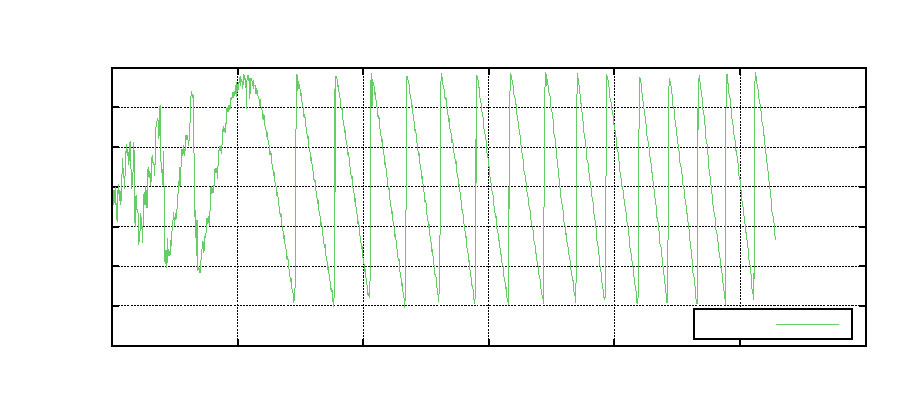
\includegraphics{diskperiastronh005q08}}%
    \gplfronttext
  \end{picture}%
\endgroup

	\end{center}
\end {figure}
\begin {figure}
	\begin{center}
		% GNUPLOT: LaTeX picture with Postscript
\begingroup
  \makeatletter
  \providecommand\color[2][]{%
    \GenericError{(gnuplot) \space\space\space\@spaces}{%
      Package color not loaded in conjunction with
      terminal option `colourtext'%
    }{See the gnuplot documentation for explanation.%
    }{Either use 'blacktext' in gnuplot or load the package
      color.sty in LaTeX.}%
    \renewcommand\color[2][]{}%
  }%
  \providecommand\includegraphics[2][]{%
    \GenericError{(gnuplot) \space\space\space\@spaces}{%
      Package graphicx or graphics not loaded%
    }{See the gnuplot documentation for explanation.%
    }{The gnuplot epslatex terminal needs graphicx.sty or graphics.sty.}%
    \renewcommand\includegraphics[2][]{}%
  }%
  \providecommand\rotatebox[2]{#2}%
  \@ifundefined{ifGPcolor}{%
    \newif\ifGPcolor
    \GPcolortrue
  }{}%
  \@ifundefined{ifGPblacktext}{%
    \newif\ifGPblacktext
    \GPblacktexttrue
  }{}%
  % define a \g@addto@macro without @ in the name:
  \let\gplgaddtomacro\g@addto@macro
  % define empty templates for all commands taking text:
  \gdef\gplbacktext{}%
  \gdef\gplfronttext{}%
  \makeatother
  \ifGPblacktext
    % no textcolor at all
    \def\colorrgb#1{}%
    \def\colorgray#1{}%
  \else
    % gray or color?
    \ifGPcolor
      \def\colorrgb#1{\color[rgb]{#1}}%
      \def\colorgray#1{\color[gray]{#1}}%
      \expandafter\def\csname LTw\endcsname{\color{white}}%
      \expandafter\def\csname LTb\endcsname{\color{black}}%
      \expandafter\def\csname LTa\endcsname{\color{black}}%
      \expandafter\def\csname LT0\endcsname{\color[rgb]{1,0,0}}%
      \expandafter\def\csname LT1\endcsname{\color[rgb]{0,1,0}}%
      \expandafter\def\csname LT2\endcsname{\color[rgb]{0,0,1}}%
      \expandafter\def\csname LT3\endcsname{\color[rgb]{1,0,1}}%
      \expandafter\def\csname LT4\endcsname{\color[rgb]{0,1,1}}%
      \expandafter\def\csname LT5\endcsname{\color[rgb]{1,1,0}}%
      \expandafter\def\csname LT6\endcsname{\color[rgb]{0,0,0}}%
      \expandafter\def\csname LT7\endcsname{\color[rgb]{1,0.3,0}}%
      \expandafter\def\csname LT8\endcsname{\color[rgb]{0.5,0.5,0.5}}%
    \else
      % gray
      \def\colorrgb#1{\color{black}}%
      \def\colorgray#1{\color[gray]{#1}}%
      \expandafter\def\csname LTw\endcsname{\color{white}}%
      \expandafter\def\csname LTb\endcsname{\color{black}}%
      \expandafter\def\csname LTa\endcsname{\color{black}}%
      \expandafter\def\csname LT0\endcsname{\color{black}}%
      \expandafter\def\csname LT1\endcsname{\color{black}}%
      \expandafter\def\csname LT2\endcsname{\color{black}}%
      \expandafter\def\csname LT3\endcsname{\color{black}}%
      \expandafter\def\csname LT4\endcsname{\color{black}}%
      \expandafter\def\csname LT5\endcsname{\color{black}}%
      \expandafter\def\csname LT6\endcsname{\color{black}}%
      \expandafter\def\csname LT7\endcsname{\color{black}}%
      \expandafter\def\csname LT8\endcsname{\color{black}}%
    \fi
  \fi
  \setlength{\unitlength}{0.0500bp}%
  \begin{picture}(8640.00,4032.00)%
    \gplgaddtomacro\gplbacktext{%
      \csname LTb\endcsname%
      \put(946,704){\makebox(0,0)[r]{\strut{}-4}}%
      \csname LTb\endcsname%
      \put(946,1085){\makebox(0,0)[r]{\strut{}-3}}%
      \csname LTb\endcsname%
      \put(946,1466){\makebox(0,0)[r]{\strut{}-2}}%
      \csname LTb\endcsname%
      \put(946,1847){\makebox(0,0)[r]{\strut{}-1}}%
      \csname LTb\endcsname%
      \put(946,2229){\makebox(0,0)[r]{\strut{} 0}}%
      \csname LTb\endcsname%
      \put(946,2610){\makebox(0,0)[r]{\strut{} 1}}%
      \csname LTb\endcsname%
      \put(946,2991){\makebox(0,0)[r]{\strut{} 2}}%
      \csname LTb\endcsname%
      \put(946,3372){\makebox(0,0)[r]{\strut{} 3}}%
      \csname LTb\endcsname%
      \put(1078,484){\makebox(0,0){\strut{} 0}}%
      \csname LTb\endcsname%
      \put(2283,484){\makebox(0,0){\strut{} 10}}%
      \csname LTb\endcsname%
      \put(3489,484){\makebox(0,0){\strut{} 20}}%
      \csname LTb\endcsname%
      \put(4694,484){\makebox(0,0){\strut{} 30}}%
      \csname LTb\endcsname%
      \put(5899,484){\makebox(0,0){\strut{} 40}}%
      \csname LTb\endcsname%
      \put(7105,484){\makebox(0,0){\strut{} 50}}%
      \csname LTb\endcsname%
      \put(8310,484){\makebox(0,0){\strut{} 60}}%
      \put(440,2038){\rotatebox{90}{\makebox(0,0){\strut{}Disk Periastron}}}%
      \put(4694,154){\makebox(0,0){\strut{}Time [$P_{\text{Orb}}$]}}%
      \put(4694,3702){\makebox(0,0){\strut{}h = 0.05}}%
    }%
    \gplgaddtomacro\gplfronttext{%
      \csname LTb\endcsname%
      \put(7323,910){\makebox(0,0)[r]{\strut{}q=0.9}}%
    }%
    \gplbacktext
    \put(0,0){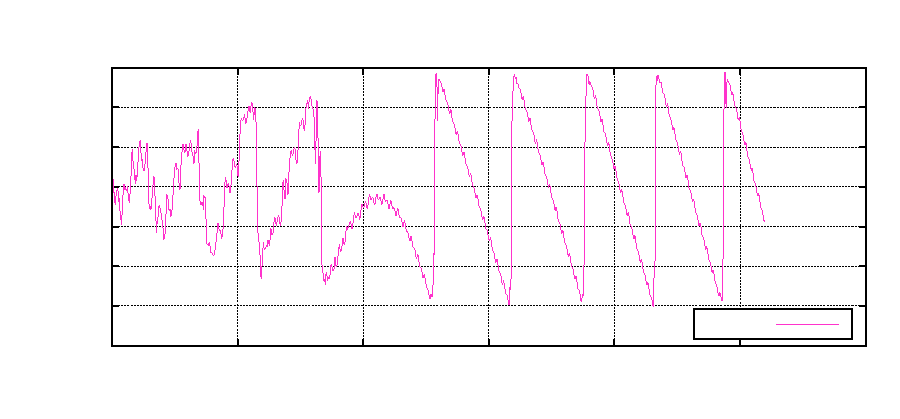
\includegraphics{diskperiastronh005q09}}%
    \gplfronttext
  \end{picture}%
\endgroup

	\end{center}
\end {figure}
\begin {figure}
	\begin{center}
		% GNUPLOT: LaTeX picture with Postscript
\begingroup
  \makeatletter
  \providecommand\color[2][]{%
    \GenericError{(gnuplot) \space\space\space\@spaces}{%
      Package color not loaded in conjunction with
      terminal option `colourtext'%
    }{See the gnuplot documentation for explanation.%
    }{Either use 'blacktext' in gnuplot or load the package
      color.sty in LaTeX.}%
    \renewcommand\color[2][]{}%
  }%
  \providecommand\includegraphics[2][]{%
    \GenericError{(gnuplot) \space\space\space\@spaces}{%
      Package graphicx or graphics not loaded%
    }{See the gnuplot documentation for explanation.%
    }{The gnuplot epslatex terminal needs graphicx.sty or graphics.sty.}%
    \renewcommand\includegraphics[2][]{}%
  }%
  \providecommand\rotatebox[2]{#2}%
  \@ifundefined{ifGPcolor}{%
    \newif\ifGPcolor
    \GPcolortrue
  }{}%
  \@ifundefined{ifGPblacktext}{%
    \newif\ifGPblacktext
    \GPblacktexttrue
  }{}%
  % define a \g@addto@macro without @ in the name:
  \let\gplgaddtomacro\g@addto@macro
  % define empty templates for all commands taking text:
  \gdef\gplbacktext{}%
  \gdef\gplfronttext{}%
  \makeatother
  \ifGPblacktext
    % no textcolor at all
    \def\colorrgb#1{}%
    \def\colorgray#1{}%
  \else
    % gray or color?
    \ifGPcolor
      \def\colorrgb#1{\color[rgb]{#1}}%
      \def\colorgray#1{\color[gray]{#1}}%
      \expandafter\def\csname LTw\endcsname{\color{white}}%
      \expandafter\def\csname LTb\endcsname{\color{black}}%
      \expandafter\def\csname LTa\endcsname{\color{black}}%
      \expandafter\def\csname LT0\endcsname{\color[rgb]{1,0,0}}%
      \expandafter\def\csname LT1\endcsname{\color[rgb]{0,1,0}}%
      \expandafter\def\csname LT2\endcsname{\color[rgb]{0,0,1}}%
      \expandafter\def\csname LT3\endcsname{\color[rgb]{1,0,1}}%
      \expandafter\def\csname LT4\endcsname{\color[rgb]{0,1,1}}%
      \expandafter\def\csname LT5\endcsname{\color[rgb]{1,1,0}}%
      \expandafter\def\csname LT6\endcsname{\color[rgb]{0,0,0}}%
      \expandafter\def\csname LT7\endcsname{\color[rgb]{1,0.3,0}}%
      \expandafter\def\csname LT8\endcsname{\color[rgb]{0.5,0.5,0.5}}%
    \else
      % gray
      \def\colorrgb#1{\color{black}}%
      \def\colorgray#1{\color[gray]{#1}}%
      \expandafter\def\csname LTw\endcsname{\color{white}}%
      \expandafter\def\csname LTb\endcsname{\color{black}}%
      \expandafter\def\csname LTa\endcsname{\color{black}}%
      \expandafter\def\csname LT0\endcsname{\color{black}}%
      \expandafter\def\csname LT1\endcsname{\color{black}}%
      \expandafter\def\csname LT2\endcsname{\color{black}}%
      \expandafter\def\csname LT3\endcsname{\color{black}}%
      \expandafter\def\csname LT4\endcsname{\color{black}}%
      \expandafter\def\csname LT5\endcsname{\color{black}}%
      \expandafter\def\csname LT6\endcsname{\color{black}}%
      \expandafter\def\csname LT7\endcsname{\color{black}}%
      \expandafter\def\csname LT8\endcsname{\color{black}}%
    \fi
  \fi
  \setlength{\unitlength}{0.0500bp}%
  \begin{picture}(8640.00,4032.00)%
    \gplgaddtomacro\gplbacktext{%
      \csname LTb\endcsname%
      \put(946,704){\makebox(0,0)[r]{\strut{}-4}}%
      \csname LTb\endcsname%
      \put(946,1085){\makebox(0,0)[r]{\strut{}-3}}%
      \csname LTb\endcsname%
      \put(946,1466){\makebox(0,0)[r]{\strut{}-2}}%
      \csname LTb\endcsname%
      \put(946,1847){\makebox(0,0)[r]{\strut{}-1}}%
      \csname LTb\endcsname%
      \put(946,2229){\makebox(0,0)[r]{\strut{} 0}}%
      \csname LTb\endcsname%
      \put(946,2610){\makebox(0,0)[r]{\strut{} 1}}%
      \csname LTb\endcsname%
      \put(946,2991){\makebox(0,0)[r]{\strut{} 2}}%
      \csname LTb\endcsname%
      \put(946,3372){\makebox(0,0)[r]{\strut{} 3}}%
      \csname LTb\endcsname%
      \put(1078,484){\makebox(0,0){\strut{} 0}}%
      \csname LTb\endcsname%
      \put(1801,484){\makebox(0,0){\strut{} 5}}%
      \csname LTb\endcsname%
      \put(2524,484){\makebox(0,0){\strut{} 10}}%
      \csname LTb\endcsname%
      \put(3248,484){\makebox(0,0){\strut{} 15}}%
      \csname LTb\endcsname%
      \put(3971,484){\makebox(0,0){\strut{} 20}}%
      \csname LTb\endcsname%
      \put(4694,484){\makebox(0,0){\strut{} 25}}%
      \csname LTb\endcsname%
      \put(5417,484){\makebox(0,0){\strut{} 30}}%
      \csname LTb\endcsname%
      \put(6140,484){\makebox(0,0){\strut{} 35}}%
      \csname LTb\endcsname%
      \put(6864,484){\makebox(0,0){\strut{} 40}}%
      \csname LTb\endcsname%
      \put(7587,484){\makebox(0,0){\strut{} 45}}%
      \csname LTb\endcsname%
      \put(8310,484){\makebox(0,0){\strut{} 50}}%
      \put(440,2038){\rotatebox{90}{\makebox(0,0){\strut{}Disk Periastron}}}%
      \put(4694,154){\makebox(0,0){\strut{}Time [$P_{\text{Orb}}$]}}%
      \put(4694,3702){\makebox(0,0){\strut{}h = 0.05}}%
    }%
    \gplgaddtomacro\gplfronttext{%
      \csname LTb\endcsname%
      \put(7323,910){\makebox(0,0)[r]{\strut{}q=1.0}}%
    }%
    \gplbacktext
    \put(0,0){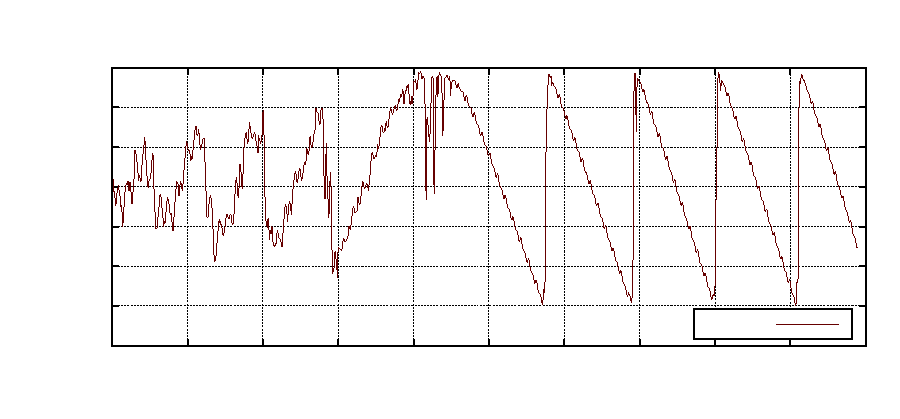
\includegraphics{diskperiastronh005q10}}%
    \gplfronttext
  \end{picture}%
\endgroup

	\end{center}
\end {figure}

\subsubsection{h = 0.04}
\begin {figure}
	\begin{center}
		% GNUPLOT: LaTeX picture with Postscript
\begingroup
  \makeatletter
  \providecommand\color[2][]{%
    \GenericError{(gnuplot) \space\space\space\@spaces}{%
      Package color not loaded in conjunction with
      terminal option `colourtext'%
    }{See the gnuplot documentation for explanation.%
    }{Either use 'blacktext' in gnuplot or load the package
      color.sty in LaTeX.}%
    \renewcommand\color[2][]{}%
  }%
  \providecommand\includegraphics[2][]{%
    \GenericError{(gnuplot) \space\space\space\@spaces}{%
      Package graphicx or graphics not loaded%
    }{See the gnuplot documentation for explanation.%
    }{The gnuplot epslatex terminal needs graphicx.sty or graphics.sty.}%
    \renewcommand\includegraphics[2][]{}%
  }%
  \providecommand\rotatebox[2]{#2}%
  \@ifundefined{ifGPcolor}{%
    \newif\ifGPcolor
    \GPcolortrue
  }{}%
  \@ifundefined{ifGPblacktext}{%
    \newif\ifGPblacktext
    \GPblacktexttrue
  }{}%
  % define a \g@addto@macro without @ in the name:
  \let\gplgaddtomacro\g@addto@macro
  % define empty templates for all commands taking text:
  \gdef\gplbacktext{}%
  \gdef\gplfronttext{}%
  \makeatother
  \ifGPblacktext
    % no textcolor at all
    \def\colorrgb#1{}%
    \def\colorgray#1{}%
  \else
    % gray or color?
    \ifGPcolor
      \def\colorrgb#1{\color[rgb]{#1}}%
      \def\colorgray#1{\color[gray]{#1}}%
      \expandafter\def\csname LTw\endcsname{\color{white}}%
      \expandafter\def\csname LTb\endcsname{\color{black}}%
      \expandafter\def\csname LTa\endcsname{\color{black}}%
      \expandafter\def\csname LT0\endcsname{\color[rgb]{1,0,0}}%
      \expandafter\def\csname LT1\endcsname{\color[rgb]{0,1,0}}%
      \expandafter\def\csname LT2\endcsname{\color[rgb]{0,0,1}}%
      \expandafter\def\csname LT3\endcsname{\color[rgb]{1,0,1}}%
      \expandafter\def\csname LT4\endcsname{\color[rgb]{0,1,1}}%
      \expandafter\def\csname LT5\endcsname{\color[rgb]{1,1,0}}%
      \expandafter\def\csname LT6\endcsname{\color[rgb]{0,0,0}}%
      \expandafter\def\csname LT7\endcsname{\color[rgb]{1,0.3,0}}%
      \expandafter\def\csname LT8\endcsname{\color[rgb]{0.5,0.5,0.5}}%
    \else
      % gray
      \def\colorrgb#1{\color{black}}%
      \def\colorgray#1{\color[gray]{#1}}%
      \expandafter\def\csname LTw\endcsname{\color{white}}%
      \expandafter\def\csname LTb\endcsname{\color{black}}%
      \expandafter\def\csname LTa\endcsname{\color{black}}%
      \expandafter\def\csname LT0\endcsname{\color{black}}%
      \expandafter\def\csname LT1\endcsname{\color{black}}%
      \expandafter\def\csname LT2\endcsname{\color{black}}%
      \expandafter\def\csname LT3\endcsname{\color{black}}%
      \expandafter\def\csname LT4\endcsname{\color{black}}%
      \expandafter\def\csname LT5\endcsname{\color{black}}%
      \expandafter\def\csname LT6\endcsname{\color{black}}%
      \expandafter\def\csname LT7\endcsname{\color{black}}%
      \expandafter\def\csname LT8\endcsname{\color{black}}%
    \fi
  \fi
  \setlength{\unitlength}{0.0500bp}%
  \begin{picture}(8640.00,4032.00)%
    \gplgaddtomacro\gplbacktext{%
      \csname LTb\endcsname%
      \put(1342,704){\makebox(0,0)[r]{\strut{} 0.28}}%
      \csname LTb\endcsname%
      \put(1342,947){\makebox(0,0)[r]{\strut{} 0.3}}%
      \csname LTb\endcsname%
      \put(1342,1189){\makebox(0,0)[r]{\strut{} 0.32}}%
      \csname LTb\endcsname%
      \put(1342,1432){\makebox(0,0)[r]{\strut{} 0.34}}%
      \csname LTb\endcsname%
      \put(1342,1674){\makebox(0,0)[r]{\strut{} 0.36}}%
      \csname LTb\endcsname%
      \put(1342,1917){\makebox(0,0)[r]{\strut{} 0.38}}%
      \csname LTb\endcsname%
      \put(1342,2159){\makebox(0,0)[r]{\strut{} 0.4}}%
      \csname LTb\endcsname%
      \put(1342,2402){\makebox(0,0)[r]{\strut{} 0.42}}%
      \csname LTb\endcsname%
      \put(1342,2644){\makebox(0,0)[r]{\strut{} 0.44}}%
      \csname LTb\endcsname%
      \put(1342,2887){\makebox(0,0)[r]{\strut{} 0.46}}%
      \csname LTb\endcsname%
      \put(1342,3129){\makebox(0,0)[r]{\strut{} 0.48}}%
      \csname LTb\endcsname%
      \put(1342,3372){\makebox(0,0)[r]{\strut{} 0.5}}%
      \csname LTb\endcsname%
      \put(1474,484){\makebox(0,0){\strut{} 0.1}}%
      \csname LTb\endcsname%
      \put(2234,484){\makebox(0,0){\strut{} 0.2}}%
      \csname LTb\endcsname%
      \put(2993,484){\makebox(0,0){\strut{} 0.3}}%
      \csname LTb\endcsname%
      \put(3753,484){\makebox(0,0){\strut{} 0.4}}%
      \csname LTb\endcsname%
      \put(4512,484){\makebox(0,0){\strut{} 0.5}}%
      \csname LTb\endcsname%
      \put(5272,484){\makebox(0,0){\strut{} 0.6}}%
      \csname LTb\endcsname%
      \put(6031,484){\makebox(0,0){\strut{} 0.7}}%
      \csname LTb\endcsname%
      \put(6791,484){\makebox(0,0){\strut{} 0.8}}%
      \csname LTb\endcsname%
      \put(7550,484){\makebox(0,0){\strut{} 0.9}}%
      \csname LTb\endcsname%
      \put(8310,484){\makebox(0,0){\strut{} 1}}%
      \put(440,2038){\rotatebox{90}{\makebox(0,0){\strut{}$\bar{\omega}$}}}%
      \put(4892,154){\makebox(0,0){\strut{}q}}%
      \put(4892,3702){\makebox(0,0){\strut{}h = 0.04}}%
    }%
    \gplgaddtomacro\gplfronttext{%
      \csname LTb\endcsname%
      \put(7323,855){\makebox(0,0)[r]{\strut{}$\bar{\omega}$}}%
    }%
    \gplbacktext
    \put(0,0){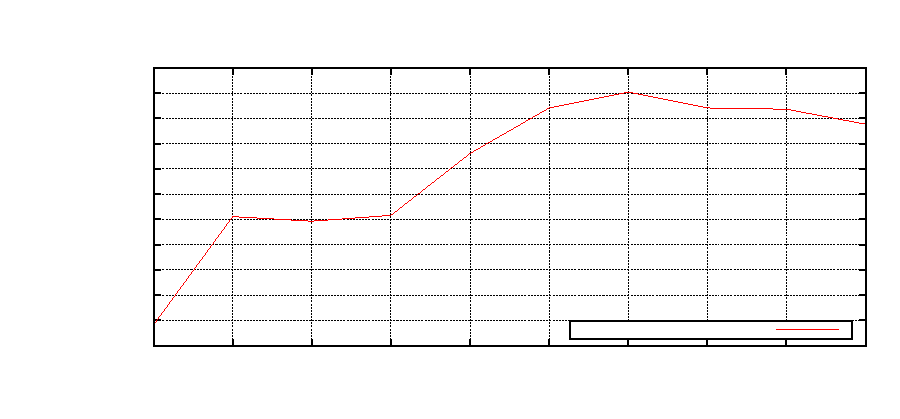
\includegraphics{diskperih004}}%
    \gplfronttext
  \end{picture}%
\endgroup

	\end{center}
	\caption{Mit zunehmendem MassRatio praezediert die Disk schneller}
\end {figure}
\begin {figure}
	\begin{center}
		% GNUPLOT: LaTeX picture with Postscript
\begingroup
  \makeatletter
  \providecommand\color[2][]{%
    \GenericError{(gnuplot) \space\space\space\@spaces}{%
      Package color not loaded in conjunction with
      terminal option `colourtext'%
    }{See the gnuplot documentation for explanation.%
    }{Either use 'blacktext' in gnuplot or load the package
      color.sty in LaTeX.}%
    \renewcommand\color[2][]{}%
  }%
  \providecommand\includegraphics[2][]{%
    \GenericError{(gnuplot) \space\space\space\@spaces}{%
      Package graphicx or graphics not loaded%
    }{See the gnuplot documentation for explanation.%
    }{The gnuplot epslatex terminal needs graphicx.sty or graphics.sty.}%
    \renewcommand\includegraphics[2][]{}%
  }%
  \providecommand\rotatebox[2]{#2}%
  \@ifundefined{ifGPcolor}{%
    \newif\ifGPcolor
    \GPcolortrue
  }{}%
  \@ifundefined{ifGPblacktext}{%
    \newif\ifGPblacktext
    \GPblacktexttrue
  }{}%
  % define a \g@addto@macro without @ in the name:
  \let\gplgaddtomacro\g@addto@macro
  % define empty templates for all commands taking text:
  \gdef\gplbacktext{}%
  \gdef\gplfronttext{}%
  \makeatother
  \ifGPblacktext
    % no textcolor at all
    \def\colorrgb#1{}%
    \def\colorgray#1{}%
  \else
    % gray or color?
    \ifGPcolor
      \def\colorrgb#1{\color[rgb]{#1}}%
      \def\colorgray#1{\color[gray]{#1}}%
      \expandafter\def\csname LTw\endcsname{\color{white}}%
      \expandafter\def\csname LTb\endcsname{\color{black}}%
      \expandafter\def\csname LTa\endcsname{\color{black}}%
      \expandafter\def\csname LT0\endcsname{\color[rgb]{1,0,0}}%
      \expandafter\def\csname LT1\endcsname{\color[rgb]{0,1,0}}%
      \expandafter\def\csname LT2\endcsname{\color[rgb]{0,0,1}}%
      \expandafter\def\csname LT3\endcsname{\color[rgb]{1,0,1}}%
      \expandafter\def\csname LT4\endcsname{\color[rgb]{0,1,1}}%
      \expandafter\def\csname LT5\endcsname{\color[rgb]{1,1,0}}%
      \expandafter\def\csname LT6\endcsname{\color[rgb]{0,0,0}}%
      \expandafter\def\csname LT7\endcsname{\color[rgb]{1,0.3,0}}%
      \expandafter\def\csname LT8\endcsname{\color[rgb]{0.5,0.5,0.5}}%
    \else
      % gray
      \def\colorrgb#1{\color{black}}%
      \def\colorgray#1{\color[gray]{#1}}%
      \expandafter\def\csname LTw\endcsname{\color{white}}%
      \expandafter\def\csname LTb\endcsname{\color{black}}%
      \expandafter\def\csname LTa\endcsname{\color{black}}%
      \expandafter\def\csname LT0\endcsname{\color{black}}%
      \expandafter\def\csname LT1\endcsname{\color{black}}%
      \expandafter\def\csname LT2\endcsname{\color{black}}%
      \expandafter\def\csname LT3\endcsname{\color{black}}%
      \expandafter\def\csname LT4\endcsname{\color{black}}%
      \expandafter\def\csname LT5\endcsname{\color{black}}%
      \expandafter\def\csname LT6\endcsname{\color{black}}%
      \expandafter\def\csname LT7\endcsname{\color{black}}%
      \expandafter\def\csname LT8\endcsname{\color{black}}%
    \fi
  \fi
  \setlength{\unitlength}{0.0500bp}%
  \begin{picture}(8640.00,4032.00)%
    \gplgaddtomacro\gplbacktext{%
      \csname LTb\endcsname%
      \put(946,704){\makebox(0,0)[r]{\strut{}-4}}%
      \csname LTb\endcsname%
      \put(946,1085){\makebox(0,0)[r]{\strut{}-3}}%
      \csname LTb\endcsname%
      \put(946,1466){\makebox(0,0)[r]{\strut{}-2}}%
      \csname LTb\endcsname%
      \put(946,1847){\makebox(0,0)[r]{\strut{}-1}}%
      \csname LTb\endcsname%
      \put(946,2229){\makebox(0,0)[r]{\strut{} 0}}%
      \csname LTb\endcsname%
      \put(946,2610){\makebox(0,0)[r]{\strut{} 1}}%
      \csname LTb\endcsname%
      \put(946,2991){\makebox(0,0)[r]{\strut{} 2}}%
      \csname LTb\endcsname%
      \put(946,3372){\makebox(0,0)[r]{\strut{} 3}}%
      \csname LTb\endcsname%
      \put(1078,484){\makebox(0,0){\strut{} 0}}%
      \csname LTb\endcsname%
      \put(1982,484){\makebox(0,0){\strut{} 20}}%
      \csname LTb\endcsname%
      \put(2886,484){\makebox(0,0){\strut{} 40}}%
      \csname LTb\endcsname%
      \put(3790,484){\makebox(0,0){\strut{} 60}}%
      \csname LTb\endcsname%
      \put(4694,484){\makebox(0,0){\strut{} 80}}%
      \csname LTb\endcsname%
      \put(5598,484){\makebox(0,0){\strut{} 100}}%
      \csname LTb\endcsname%
      \put(6502,484){\makebox(0,0){\strut{} 120}}%
      \csname LTb\endcsname%
      \put(7406,484){\makebox(0,0){\strut{} 140}}%
      \csname LTb\endcsname%
      \put(8310,484){\makebox(0,0){\strut{} 160}}%
      \put(440,2038){\rotatebox{90}{\makebox(0,0){\strut{}Disk Periastron}}}%
      \put(4694,154){\makebox(0,0){\strut{}Time [$P_{\text{Orb}}$]}}%
      \put(4694,3702){\makebox(0,0){\strut{}h = 0.04}}%
    }%
    \gplgaddtomacro\gplfronttext{%
      \csname LTb\endcsname%
      \put(7323,910){\makebox(0,0)[r]{\strut{}q=0.1}}%
    }%
    \gplbacktext
    \put(0,0){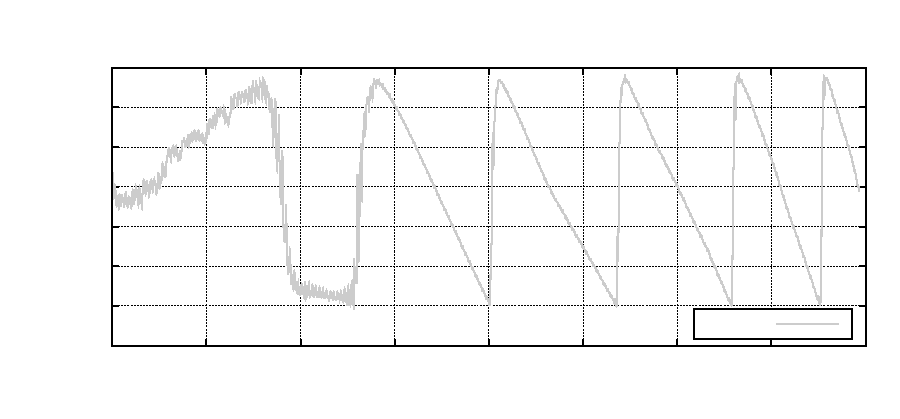
\includegraphics{diskperiastronh004q01}}%
    \gplfronttext
  \end{picture}%
\endgroup

	\end{center}
\end {figure}
\begin {figure}
	\begin{center}
		% GNUPLOT: LaTeX picture with Postscript
\begingroup
  \makeatletter
  \providecommand\color[2][]{%
    \GenericError{(gnuplot) \space\space\space\@spaces}{%
      Package color not loaded in conjunction with
      terminal option `colourtext'%
    }{See the gnuplot documentation for explanation.%
    }{Either use 'blacktext' in gnuplot or load the package
      color.sty in LaTeX.}%
    \renewcommand\color[2][]{}%
  }%
  \providecommand\includegraphics[2][]{%
    \GenericError{(gnuplot) \space\space\space\@spaces}{%
      Package graphicx or graphics not loaded%
    }{See the gnuplot documentation for explanation.%
    }{The gnuplot epslatex terminal needs graphicx.sty or graphics.sty.}%
    \renewcommand\includegraphics[2][]{}%
  }%
  \providecommand\rotatebox[2]{#2}%
  \@ifundefined{ifGPcolor}{%
    \newif\ifGPcolor
    \GPcolortrue
  }{}%
  \@ifundefined{ifGPblacktext}{%
    \newif\ifGPblacktext
    \GPblacktexttrue
  }{}%
  % define a \g@addto@macro without @ in the name:
  \let\gplgaddtomacro\g@addto@macro
  % define empty templates for all commands taking text:
  \gdef\gplbacktext{}%
  \gdef\gplfronttext{}%
  \makeatother
  \ifGPblacktext
    % no textcolor at all
    \def\colorrgb#1{}%
    \def\colorgray#1{}%
  \else
    % gray or color?
    \ifGPcolor
      \def\colorrgb#1{\color[rgb]{#1}}%
      \def\colorgray#1{\color[gray]{#1}}%
      \expandafter\def\csname LTw\endcsname{\color{white}}%
      \expandafter\def\csname LTb\endcsname{\color{black}}%
      \expandafter\def\csname LTa\endcsname{\color{black}}%
      \expandafter\def\csname LT0\endcsname{\color[rgb]{1,0,0}}%
      \expandafter\def\csname LT1\endcsname{\color[rgb]{0,1,0}}%
      \expandafter\def\csname LT2\endcsname{\color[rgb]{0,0,1}}%
      \expandafter\def\csname LT3\endcsname{\color[rgb]{1,0,1}}%
      \expandafter\def\csname LT4\endcsname{\color[rgb]{0,1,1}}%
      \expandafter\def\csname LT5\endcsname{\color[rgb]{1,1,0}}%
      \expandafter\def\csname LT6\endcsname{\color[rgb]{0,0,0}}%
      \expandafter\def\csname LT7\endcsname{\color[rgb]{1,0.3,0}}%
      \expandafter\def\csname LT8\endcsname{\color[rgb]{0.5,0.5,0.5}}%
    \else
      % gray
      \def\colorrgb#1{\color{black}}%
      \def\colorgray#1{\color[gray]{#1}}%
      \expandafter\def\csname LTw\endcsname{\color{white}}%
      \expandafter\def\csname LTb\endcsname{\color{black}}%
      \expandafter\def\csname LTa\endcsname{\color{black}}%
      \expandafter\def\csname LT0\endcsname{\color{black}}%
      \expandafter\def\csname LT1\endcsname{\color{black}}%
      \expandafter\def\csname LT2\endcsname{\color{black}}%
      \expandafter\def\csname LT3\endcsname{\color{black}}%
      \expandafter\def\csname LT4\endcsname{\color{black}}%
      \expandafter\def\csname LT5\endcsname{\color{black}}%
      \expandafter\def\csname LT6\endcsname{\color{black}}%
      \expandafter\def\csname LT7\endcsname{\color{black}}%
      \expandafter\def\csname LT8\endcsname{\color{black}}%
    \fi
  \fi
  \setlength{\unitlength}{0.0500bp}%
  \begin{picture}(8640.00,4032.00)%
    \gplgaddtomacro\gplbacktext{%
      \csname LTb\endcsname%
      \put(946,704){\makebox(0,0)[r]{\strut{}-4}}%
      \csname LTb\endcsname%
      \put(946,1085){\makebox(0,0)[r]{\strut{}-3}}%
      \csname LTb\endcsname%
      \put(946,1466){\makebox(0,0)[r]{\strut{}-2}}%
      \csname LTb\endcsname%
      \put(946,1847){\makebox(0,0)[r]{\strut{}-1}}%
      \csname LTb\endcsname%
      \put(946,2229){\makebox(0,0)[r]{\strut{} 0}}%
      \csname LTb\endcsname%
      \put(946,2610){\makebox(0,0)[r]{\strut{} 1}}%
      \csname LTb\endcsname%
      \put(946,2991){\makebox(0,0)[r]{\strut{} 2}}%
      \csname LTb\endcsname%
      \put(946,3372){\makebox(0,0)[r]{\strut{} 3}}%
      \csname LTb\endcsname%
      \put(1078,484){\makebox(0,0){\strut{} 0}}%
      \csname LTb\endcsname%
      \put(1982,484){\makebox(0,0){\strut{} 20}}%
      \csname LTb\endcsname%
      \put(2886,484){\makebox(0,0){\strut{} 40}}%
      \csname LTb\endcsname%
      \put(3790,484){\makebox(0,0){\strut{} 60}}%
      \csname LTb\endcsname%
      \put(4694,484){\makebox(0,0){\strut{} 80}}%
      \csname LTb\endcsname%
      \put(5598,484){\makebox(0,0){\strut{} 100}}%
      \csname LTb\endcsname%
      \put(6502,484){\makebox(0,0){\strut{} 120}}%
      \csname LTb\endcsname%
      \put(7406,484){\makebox(0,0){\strut{} 140}}%
      \csname LTb\endcsname%
      \put(8310,484){\makebox(0,0){\strut{} 160}}%
      \put(440,2038){\rotatebox{90}{\makebox(0,0){\strut{}Disk Periastron}}}%
      \put(4694,154){\makebox(0,0){\strut{}Time [$P_{\text{Orb}}$]}}%
      \put(4694,3702){\makebox(0,0){\strut{}h = 0.04}}%
    }%
    \gplgaddtomacro\gplfronttext{%
      \csname LTb\endcsname%
      \put(7323,910){\makebox(0,0)[r]{\strut{}q=0.2}}%
    }%
    \gplbacktext
    \put(0,0){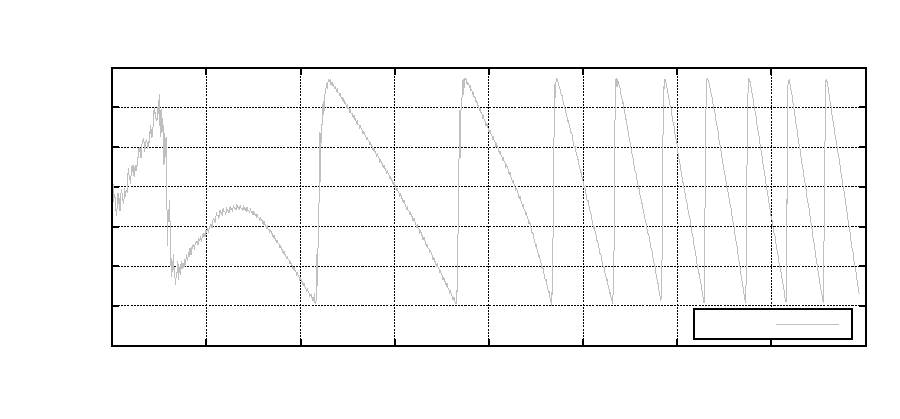
\includegraphics{diskperiastronh004q02}}%
    \gplfronttext
  \end{picture}%
\endgroup

	\end{center}
\end {figure}
\begin {figure}
	\begin{center}
		% GNUPLOT: LaTeX picture with Postscript
\begingroup
  \makeatletter
  \providecommand\color[2][]{%
    \GenericError{(gnuplot) \space\space\space\@spaces}{%
      Package color not loaded in conjunction with
      terminal option `colourtext'%
    }{See the gnuplot documentation for explanation.%
    }{Either use 'blacktext' in gnuplot or load the package
      color.sty in LaTeX.}%
    \renewcommand\color[2][]{}%
  }%
  \providecommand\includegraphics[2][]{%
    \GenericError{(gnuplot) \space\space\space\@spaces}{%
      Package graphicx or graphics not loaded%
    }{See the gnuplot documentation for explanation.%
    }{The gnuplot epslatex terminal needs graphicx.sty or graphics.sty.}%
    \renewcommand\includegraphics[2][]{}%
  }%
  \providecommand\rotatebox[2]{#2}%
  \@ifundefined{ifGPcolor}{%
    \newif\ifGPcolor
    \GPcolortrue
  }{}%
  \@ifundefined{ifGPblacktext}{%
    \newif\ifGPblacktext
    \GPblacktexttrue
  }{}%
  % define a \g@addto@macro without @ in the name:
  \let\gplgaddtomacro\g@addto@macro
  % define empty templates for all commands taking text:
  \gdef\gplbacktext{}%
  \gdef\gplfronttext{}%
  \makeatother
  \ifGPblacktext
    % no textcolor at all
    \def\colorrgb#1{}%
    \def\colorgray#1{}%
  \else
    % gray or color?
    \ifGPcolor
      \def\colorrgb#1{\color[rgb]{#1}}%
      \def\colorgray#1{\color[gray]{#1}}%
      \expandafter\def\csname LTw\endcsname{\color{white}}%
      \expandafter\def\csname LTb\endcsname{\color{black}}%
      \expandafter\def\csname LTa\endcsname{\color{black}}%
      \expandafter\def\csname LT0\endcsname{\color[rgb]{1,0,0}}%
      \expandafter\def\csname LT1\endcsname{\color[rgb]{0,1,0}}%
      \expandafter\def\csname LT2\endcsname{\color[rgb]{0,0,1}}%
      \expandafter\def\csname LT3\endcsname{\color[rgb]{1,0,1}}%
      \expandafter\def\csname LT4\endcsname{\color[rgb]{0,1,1}}%
      \expandafter\def\csname LT5\endcsname{\color[rgb]{1,1,0}}%
      \expandafter\def\csname LT6\endcsname{\color[rgb]{0,0,0}}%
      \expandafter\def\csname LT7\endcsname{\color[rgb]{1,0.3,0}}%
      \expandafter\def\csname LT8\endcsname{\color[rgb]{0.5,0.5,0.5}}%
    \else
      % gray
      \def\colorrgb#1{\color{black}}%
      \def\colorgray#1{\color[gray]{#1}}%
      \expandafter\def\csname LTw\endcsname{\color{white}}%
      \expandafter\def\csname LTb\endcsname{\color{black}}%
      \expandafter\def\csname LTa\endcsname{\color{black}}%
      \expandafter\def\csname LT0\endcsname{\color{black}}%
      \expandafter\def\csname LT1\endcsname{\color{black}}%
      \expandafter\def\csname LT2\endcsname{\color{black}}%
      \expandafter\def\csname LT3\endcsname{\color{black}}%
      \expandafter\def\csname LT4\endcsname{\color{black}}%
      \expandafter\def\csname LT5\endcsname{\color{black}}%
      \expandafter\def\csname LT6\endcsname{\color{black}}%
      \expandafter\def\csname LT7\endcsname{\color{black}}%
      \expandafter\def\csname LT8\endcsname{\color{black}}%
    \fi
  \fi
  \setlength{\unitlength}{0.0500bp}%
  \begin{picture}(8640.00,4032.00)%
    \gplgaddtomacro\gplbacktext{%
      \csname LTb\endcsname%
      \put(946,704){\makebox(0,0)[r]{\strut{}-3}}%
      \csname LTb\endcsname%
      \put(946,1149){\makebox(0,0)[r]{\strut{}-2}}%
      \csname LTb\endcsname%
      \put(946,1593){\makebox(0,0)[r]{\strut{}-1}}%
      \csname LTb\endcsname%
      \put(946,2038){\makebox(0,0)[r]{\strut{} 0}}%
      \csname LTb\endcsname%
      \put(946,2483){\makebox(0,0)[r]{\strut{} 1}}%
      \csname LTb\endcsname%
      \put(946,2927){\makebox(0,0)[r]{\strut{} 2}}%
      \csname LTb\endcsname%
      \put(946,3372){\makebox(0,0)[r]{\strut{} 3}}%
      \csname LTb\endcsname%
      \put(1078,484){\makebox(0,0){\strut{} 0}}%
      \csname LTb\endcsname%
      \put(1982,484){\makebox(0,0){\strut{} 20}}%
      \csname LTb\endcsname%
      \put(2886,484){\makebox(0,0){\strut{} 40}}%
      \csname LTb\endcsname%
      \put(3790,484){\makebox(0,0){\strut{} 60}}%
      \csname LTb\endcsname%
      \put(4694,484){\makebox(0,0){\strut{} 80}}%
      \csname LTb\endcsname%
      \put(5598,484){\makebox(0,0){\strut{} 100}}%
      \csname LTb\endcsname%
      \put(6502,484){\makebox(0,0){\strut{} 120}}%
      \csname LTb\endcsname%
      \put(7406,484){\makebox(0,0){\strut{} 140}}%
      \csname LTb\endcsname%
      \put(8310,484){\makebox(0,0){\strut{} 160}}%
      \put(440,2038){\rotatebox{90}{\makebox(0,0){\strut{}Disk Periastron}}}%
      \put(4694,154){\makebox(0,0){\strut{}Time [$P_{\text{Orb}}$]}}%
      \put(4694,3702){\makebox(0,0){\strut{}h = 0.04}}%
    }%
    \gplgaddtomacro\gplfronttext{%
      \csname LTb\endcsname%
      \put(7323,910){\makebox(0,0)[r]{\strut{}q=0.3}}%
    }%
    \gplbacktext
    \put(0,0){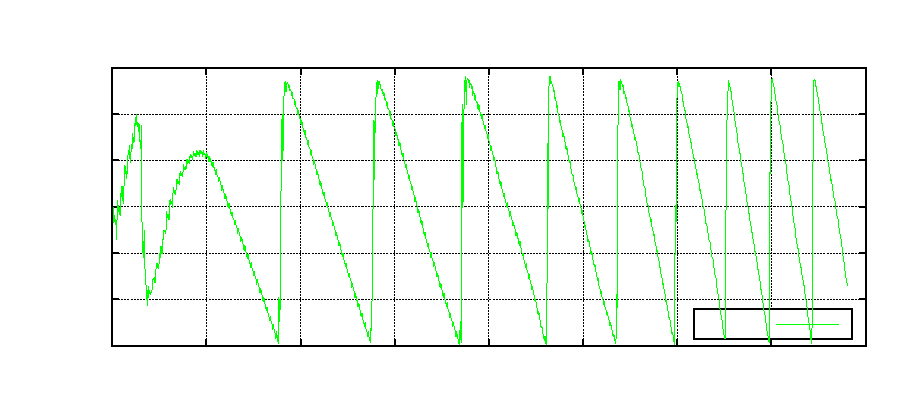
\includegraphics{diskperiastronh004q03}}%
    \gplfronttext
  \end{picture}%
\endgroup

	\end{center}
\end {figure}
\begin {figure}
	\begin{center}
		% GNUPLOT: LaTeX picture with Postscript
\begingroup
  \makeatletter
  \providecommand\color[2][]{%
    \GenericError{(gnuplot) \space\space\space\@spaces}{%
      Package color not loaded in conjunction with
      terminal option `colourtext'%
    }{See the gnuplot documentation for explanation.%
    }{Either use 'blacktext' in gnuplot or load the package
      color.sty in LaTeX.}%
    \renewcommand\color[2][]{}%
  }%
  \providecommand\includegraphics[2][]{%
    \GenericError{(gnuplot) \space\space\space\@spaces}{%
      Package graphicx or graphics not loaded%
    }{See the gnuplot documentation for explanation.%
    }{The gnuplot epslatex terminal needs graphicx.sty or graphics.sty.}%
    \renewcommand\includegraphics[2][]{}%
  }%
  \providecommand\rotatebox[2]{#2}%
  \@ifundefined{ifGPcolor}{%
    \newif\ifGPcolor
    \GPcolortrue
  }{}%
  \@ifundefined{ifGPblacktext}{%
    \newif\ifGPblacktext
    \GPblacktexttrue
  }{}%
  % define a \g@addto@macro without @ in the name:
  \let\gplgaddtomacro\g@addto@macro
  % define empty templates for all commands taking text:
  \gdef\gplbacktext{}%
  \gdef\gplfronttext{}%
  \makeatother
  \ifGPblacktext
    % no textcolor at all
    \def\colorrgb#1{}%
    \def\colorgray#1{}%
  \else
    % gray or color?
    \ifGPcolor
      \def\colorrgb#1{\color[rgb]{#1}}%
      \def\colorgray#1{\color[gray]{#1}}%
      \expandafter\def\csname LTw\endcsname{\color{white}}%
      \expandafter\def\csname LTb\endcsname{\color{black}}%
      \expandafter\def\csname LTa\endcsname{\color{black}}%
      \expandafter\def\csname LT0\endcsname{\color[rgb]{1,0,0}}%
      \expandafter\def\csname LT1\endcsname{\color[rgb]{0,1,0}}%
      \expandafter\def\csname LT2\endcsname{\color[rgb]{0,0,1}}%
      \expandafter\def\csname LT3\endcsname{\color[rgb]{1,0,1}}%
      \expandafter\def\csname LT4\endcsname{\color[rgb]{0,1,1}}%
      \expandafter\def\csname LT5\endcsname{\color[rgb]{1,1,0}}%
      \expandafter\def\csname LT6\endcsname{\color[rgb]{0,0,0}}%
      \expandafter\def\csname LT7\endcsname{\color[rgb]{1,0.3,0}}%
      \expandafter\def\csname LT8\endcsname{\color[rgb]{0.5,0.5,0.5}}%
    \else
      % gray
      \def\colorrgb#1{\color{black}}%
      \def\colorgray#1{\color[gray]{#1}}%
      \expandafter\def\csname LTw\endcsname{\color{white}}%
      \expandafter\def\csname LTb\endcsname{\color{black}}%
      \expandafter\def\csname LTa\endcsname{\color{black}}%
      \expandafter\def\csname LT0\endcsname{\color{black}}%
      \expandafter\def\csname LT1\endcsname{\color{black}}%
      \expandafter\def\csname LT2\endcsname{\color{black}}%
      \expandafter\def\csname LT3\endcsname{\color{black}}%
      \expandafter\def\csname LT4\endcsname{\color{black}}%
      \expandafter\def\csname LT5\endcsname{\color{black}}%
      \expandafter\def\csname LT6\endcsname{\color{black}}%
      \expandafter\def\csname LT7\endcsname{\color{black}}%
      \expandafter\def\csname LT8\endcsname{\color{black}}%
    \fi
  \fi
  \setlength{\unitlength}{0.0500bp}%
  \begin{picture}(8640.00,4032.00)%
    \gplgaddtomacro\gplbacktext{%
      \csname LTb\endcsname%
      \put(946,704){\makebox(0,0)[r]{\strut{}-4}}%
      \csname LTb\endcsname%
      \put(946,1085){\makebox(0,0)[r]{\strut{}-3}}%
      \csname LTb\endcsname%
      \put(946,1466){\makebox(0,0)[r]{\strut{}-2}}%
      \csname LTb\endcsname%
      \put(946,1847){\makebox(0,0)[r]{\strut{}-1}}%
      \csname LTb\endcsname%
      \put(946,2229){\makebox(0,0)[r]{\strut{} 0}}%
      \csname LTb\endcsname%
      \put(946,2610){\makebox(0,0)[r]{\strut{} 1}}%
      \csname LTb\endcsname%
      \put(946,2991){\makebox(0,0)[r]{\strut{} 2}}%
      \csname LTb\endcsname%
      \put(946,3372){\makebox(0,0)[r]{\strut{} 3}}%
      \csname LTb\endcsname%
      \put(1078,484){\makebox(0,0){\strut{} 0}}%
      \csname LTb\endcsname%
      \put(2111,484){\makebox(0,0){\strut{} 20}}%
      \csname LTb\endcsname%
      \put(3144,484){\makebox(0,0){\strut{} 40}}%
      \csname LTb\endcsname%
      \put(4177,484){\makebox(0,0){\strut{} 60}}%
      \csname LTb\endcsname%
      \put(5211,484){\makebox(0,0){\strut{} 80}}%
      \csname LTb\endcsname%
      \put(6244,484){\makebox(0,0){\strut{} 100}}%
      \csname LTb\endcsname%
      \put(7277,484){\makebox(0,0){\strut{} 120}}%
      \csname LTb\endcsname%
      \put(8310,484){\makebox(0,0){\strut{} 140}}%
      \put(440,2038){\rotatebox{90}{\makebox(0,0){\strut{}Disk Periastron}}}%
      \put(4694,154){\makebox(0,0){\strut{}Time [$P_{\text{Orb}}$]}}%
      \put(4694,3702){\makebox(0,0){\strut{}h = 0.04}}%
    }%
    \gplgaddtomacro\gplfronttext{%
      \csname LTb\endcsname%
      \put(7323,910){\makebox(0,0)[r]{\strut{}q=0.4}}%
    }%
    \gplbacktext
    \put(0,0){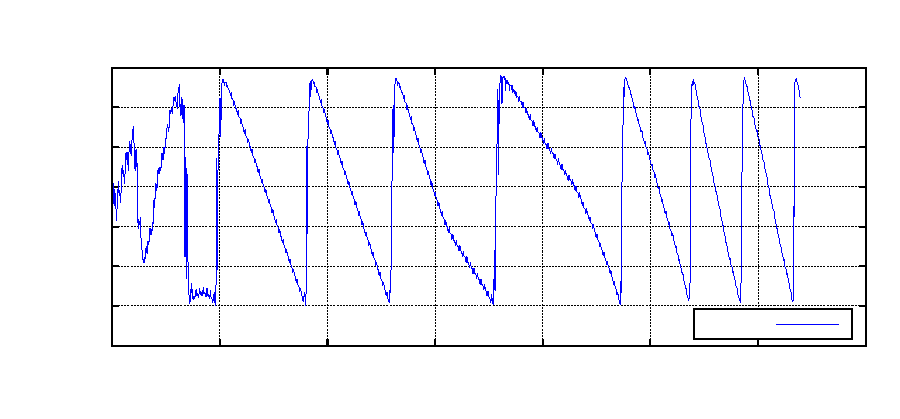
\includegraphics{diskperiastronh004q04}}%
    \gplfronttext
  \end{picture}%
\endgroup

	\end{center}
\end {figure}
\begin {figure}
	\begin{center}
		% GNUPLOT: LaTeX picture with Postscript
\begingroup
  \makeatletter
  \providecommand\color[2][]{%
    \GenericError{(gnuplot) \space\space\space\@spaces}{%
      Package color not loaded in conjunction with
      terminal option `colourtext'%
    }{See the gnuplot documentation for explanation.%
    }{Either use 'blacktext' in gnuplot or load the package
      color.sty in LaTeX.}%
    \renewcommand\color[2][]{}%
  }%
  \providecommand\includegraphics[2][]{%
    \GenericError{(gnuplot) \space\space\space\@spaces}{%
      Package graphicx or graphics not loaded%
    }{See the gnuplot documentation for explanation.%
    }{The gnuplot epslatex terminal needs graphicx.sty or graphics.sty.}%
    \renewcommand\includegraphics[2][]{}%
  }%
  \providecommand\rotatebox[2]{#2}%
  \@ifundefined{ifGPcolor}{%
    \newif\ifGPcolor
    \GPcolortrue
  }{}%
  \@ifundefined{ifGPblacktext}{%
    \newif\ifGPblacktext
    \GPblacktexttrue
  }{}%
  % define a \g@addto@macro without @ in the name:
  \let\gplgaddtomacro\g@addto@macro
  % define empty templates for all commands taking text:
  \gdef\gplbacktext{}%
  \gdef\gplfronttext{}%
  \makeatother
  \ifGPblacktext
    % no textcolor at all
    \def\colorrgb#1{}%
    \def\colorgray#1{}%
  \else
    % gray or color?
    \ifGPcolor
      \def\colorrgb#1{\color[rgb]{#1}}%
      \def\colorgray#1{\color[gray]{#1}}%
      \expandafter\def\csname LTw\endcsname{\color{white}}%
      \expandafter\def\csname LTb\endcsname{\color{black}}%
      \expandafter\def\csname LTa\endcsname{\color{black}}%
      \expandafter\def\csname LT0\endcsname{\color[rgb]{1,0,0}}%
      \expandafter\def\csname LT1\endcsname{\color[rgb]{0,1,0}}%
      \expandafter\def\csname LT2\endcsname{\color[rgb]{0,0,1}}%
      \expandafter\def\csname LT3\endcsname{\color[rgb]{1,0,1}}%
      \expandafter\def\csname LT4\endcsname{\color[rgb]{0,1,1}}%
      \expandafter\def\csname LT5\endcsname{\color[rgb]{1,1,0}}%
      \expandafter\def\csname LT6\endcsname{\color[rgb]{0,0,0}}%
      \expandafter\def\csname LT7\endcsname{\color[rgb]{1,0.3,0}}%
      \expandafter\def\csname LT8\endcsname{\color[rgb]{0.5,0.5,0.5}}%
    \else
      % gray
      \def\colorrgb#1{\color{black}}%
      \def\colorgray#1{\color[gray]{#1}}%
      \expandafter\def\csname LTw\endcsname{\color{white}}%
      \expandafter\def\csname LTb\endcsname{\color{black}}%
      \expandafter\def\csname LTa\endcsname{\color{black}}%
      \expandafter\def\csname LT0\endcsname{\color{black}}%
      \expandafter\def\csname LT1\endcsname{\color{black}}%
      \expandafter\def\csname LT2\endcsname{\color{black}}%
      \expandafter\def\csname LT3\endcsname{\color{black}}%
      \expandafter\def\csname LT4\endcsname{\color{black}}%
      \expandafter\def\csname LT5\endcsname{\color{black}}%
      \expandafter\def\csname LT6\endcsname{\color{black}}%
      \expandafter\def\csname LT7\endcsname{\color{black}}%
      \expandafter\def\csname LT8\endcsname{\color{black}}%
    \fi
  \fi
  \setlength{\unitlength}{0.0500bp}%
  \begin{picture}(8640.00,4032.00)%
    \gplgaddtomacro\gplbacktext{%
      \csname LTb\endcsname%
      \put(946,704){\makebox(0,0)[r]{\strut{}-3}}%
      \csname LTb\endcsname%
      \put(946,1149){\makebox(0,0)[r]{\strut{}-2}}%
      \csname LTb\endcsname%
      \put(946,1593){\makebox(0,0)[r]{\strut{}-1}}%
      \csname LTb\endcsname%
      \put(946,2038){\makebox(0,0)[r]{\strut{} 0}}%
      \csname LTb\endcsname%
      \put(946,2483){\makebox(0,0)[r]{\strut{} 1}}%
      \csname LTb\endcsname%
      \put(946,2927){\makebox(0,0)[r]{\strut{} 2}}%
      \csname LTb\endcsname%
      \put(946,3372){\makebox(0,0)[r]{\strut{} 3}}%
      \csname LTb\endcsname%
      \put(1078,484){\makebox(0,0){\strut{} 0}}%
      \csname LTb\endcsname%
      \put(2111,484){\makebox(0,0){\strut{} 20}}%
      \csname LTb\endcsname%
      \put(3144,484){\makebox(0,0){\strut{} 40}}%
      \csname LTb\endcsname%
      \put(4177,484){\makebox(0,0){\strut{} 60}}%
      \csname LTb\endcsname%
      \put(5211,484){\makebox(0,0){\strut{} 80}}%
      \csname LTb\endcsname%
      \put(6244,484){\makebox(0,0){\strut{} 100}}%
      \csname LTb\endcsname%
      \put(7277,484){\makebox(0,0){\strut{} 120}}%
      \csname LTb\endcsname%
      \put(8310,484){\makebox(0,0){\strut{} 140}}%
      \put(440,2038){\rotatebox{90}{\makebox(0,0){\strut{}Disk Periastron}}}%
      \put(4694,154){\makebox(0,0){\strut{}Time [$P_{\text{Orb}}$]}}%
      \put(4694,3702){\makebox(0,0){\strut{}h = 0.04}}%
    }%
    \gplgaddtomacro\gplfronttext{%
      \csname LTb\endcsname%
      \put(7323,910){\makebox(0,0)[r]{\strut{}q=0.5}}%
    }%
    \gplbacktext
    \put(0,0){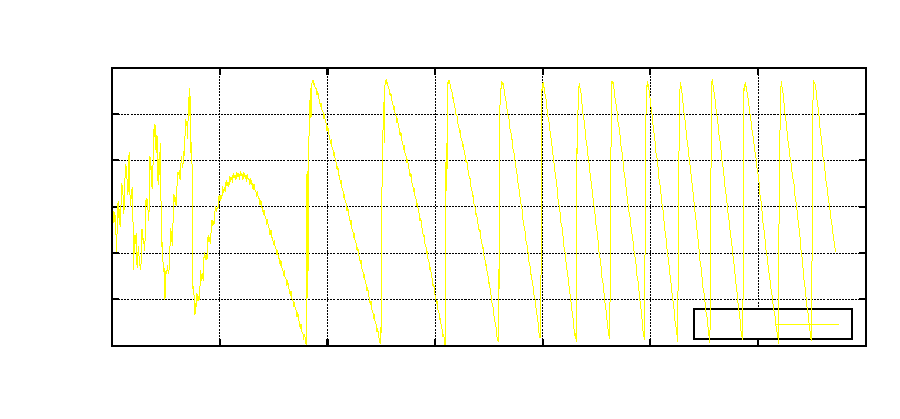
\includegraphics{diskperiastronh004q05}}%
    \gplfronttext
  \end{picture}%
\endgroup

	\end{center}
\end {figure}
\begin {figure}
	\begin{center}
		% GNUPLOT: LaTeX picture with Postscript
\begingroup
  \makeatletter
  \providecommand\color[2][]{%
    \GenericError{(gnuplot) \space\space\space\@spaces}{%
      Package color not loaded in conjunction with
      terminal option `colourtext'%
    }{See the gnuplot documentation for explanation.%
    }{Either use 'blacktext' in gnuplot or load the package
      color.sty in LaTeX.}%
    \renewcommand\color[2][]{}%
  }%
  \providecommand\includegraphics[2][]{%
    \GenericError{(gnuplot) \space\space\space\@spaces}{%
      Package graphicx or graphics not loaded%
    }{See the gnuplot documentation for explanation.%
    }{The gnuplot epslatex terminal needs graphicx.sty or graphics.sty.}%
    \renewcommand\includegraphics[2][]{}%
  }%
  \providecommand\rotatebox[2]{#2}%
  \@ifundefined{ifGPcolor}{%
    \newif\ifGPcolor
    \GPcolortrue
  }{}%
  \@ifundefined{ifGPblacktext}{%
    \newif\ifGPblacktext
    \GPblacktexttrue
  }{}%
  % define a \g@addto@macro without @ in the name:
  \let\gplgaddtomacro\g@addto@macro
  % define empty templates for all commands taking text:
  \gdef\gplbacktext{}%
  \gdef\gplfronttext{}%
  \makeatother
  \ifGPblacktext
    % no textcolor at all
    \def\colorrgb#1{}%
    \def\colorgray#1{}%
  \else
    % gray or color?
    \ifGPcolor
      \def\colorrgb#1{\color[rgb]{#1}}%
      \def\colorgray#1{\color[gray]{#1}}%
      \expandafter\def\csname LTw\endcsname{\color{white}}%
      \expandafter\def\csname LTb\endcsname{\color{black}}%
      \expandafter\def\csname LTa\endcsname{\color{black}}%
      \expandafter\def\csname LT0\endcsname{\color[rgb]{1,0,0}}%
      \expandafter\def\csname LT1\endcsname{\color[rgb]{0,1,0}}%
      \expandafter\def\csname LT2\endcsname{\color[rgb]{0,0,1}}%
      \expandafter\def\csname LT3\endcsname{\color[rgb]{1,0,1}}%
      \expandafter\def\csname LT4\endcsname{\color[rgb]{0,1,1}}%
      \expandafter\def\csname LT5\endcsname{\color[rgb]{1,1,0}}%
      \expandafter\def\csname LT6\endcsname{\color[rgb]{0,0,0}}%
      \expandafter\def\csname LT7\endcsname{\color[rgb]{1,0.3,0}}%
      \expandafter\def\csname LT8\endcsname{\color[rgb]{0.5,0.5,0.5}}%
    \else
      % gray
      \def\colorrgb#1{\color{black}}%
      \def\colorgray#1{\color[gray]{#1}}%
      \expandafter\def\csname LTw\endcsname{\color{white}}%
      \expandafter\def\csname LTb\endcsname{\color{black}}%
      \expandafter\def\csname LTa\endcsname{\color{black}}%
      \expandafter\def\csname LT0\endcsname{\color{black}}%
      \expandafter\def\csname LT1\endcsname{\color{black}}%
      \expandafter\def\csname LT2\endcsname{\color{black}}%
      \expandafter\def\csname LT3\endcsname{\color{black}}%
      \expandafter\def\csname LT4\endcsname{\color{black}}%
      \expandafter\def\csname LT5\endcsname{\color{black}}%
      \expandafter\def\csname LT6\endcsname{\color{black}}%
      \expandafter\def\csname LT7\endcsname{\color{black}}%
      \expandafter\def\csname LT8\endcsname{\color{black}}%
    \fi
  \fi
  \setlength{\unitlength}{0.0500bp}%
  \begin{picture}(8640.00,4032.00)%
    \gplgaddtomacro\gplbacktext{%
      \csname LTb\endcsname%
      \put(946,704){\makebox(0,0)[r]{\strut{}-3}}%
      \csname LTb\endcsname%
      \put(946,1149){\makebox(0,0)[r]{\strut{}-2}}%
      \csname LTb\endcsname%
      \put(946,1593){\makebox(0,0)[r]{\strut{}-1}}%
      \csname LTb\endcsname%
      \put(946,2038){\makebox(0,0)[r]{\strut{} 0}}%
      \csname LTb\endcsname%
      \put(946,2483){\makebox(0,0)[r]{\strut{} 1}}%
      \csname LTb\endcsname%
      \put(946,2927){\makebox(0,0)[r]{\strut{} 2}}%
      \csname LTb\endcsname%
      \put(946,3372){\makebox(0,0)[r]{\strut{} 3}}%
      \csname LTb\endcsname%
      \put(1078,484){\makebox(0,0){\strut{} 0}}%
      \csname LTb\endcsname%
      \put(2111,484){\makebox(0,0){\strut{} 20}}%
      \csname LTb\endcsname%
      \put(3144,484){\makebox(0,0){\strut{} 40}}%
      \csname LTb\endcsname%
      \put(4177,484){\makebox(0,0){\strut{} 60}}%
      \csname LTb\endcsname%
      \put(5211,484){\makebox(0,0){\strut{} 80}}%
      \csname LTb\endcsname%
      \put(6244,484){\makebox(0,0){\strut{} 100}}%
      \csname LTb\endcsname%
      \put(7277,484){\makebox(0,0){\strut{} 120}}%
      \csname LTb\endcsname%
      \put(8310,484){\makebox(0,0){\strut{} 140}}%
      \put(440,2038){\rotatebox{90}{\makebox(0,0){\strut{}Disk Periastron}}}%
      \put(4694,154){\makebox(0,0){\strut{}Time [$P_{\text{Orb}}$]}}%
      \put(4694,3702){\makebox(0,0){\strut{}h = 0.04}}%
    }%
    \gplgaddtomacro\gplfronttext{%
      \csname LTb\endcsname%
      \put(7323,910){\makebox(0,0)[r]{\strut{}q=0.6}}%
    }%
    \gplbacktext
    \put(0,0){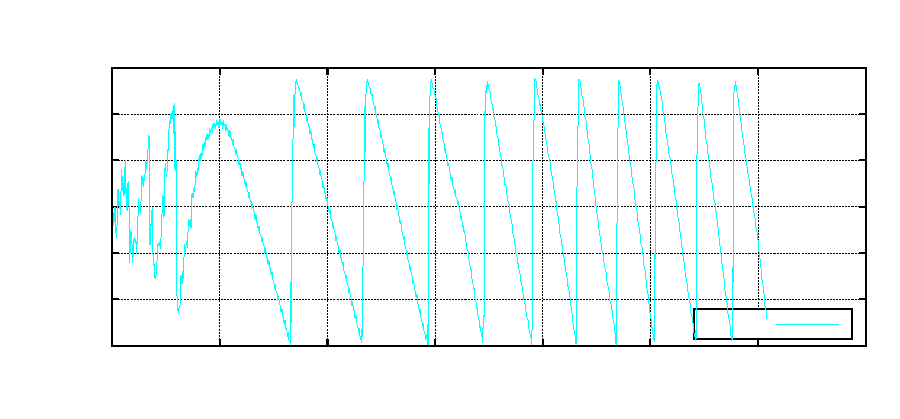
\includegraphics{diskperiastronh004q06}}%
    \gplfronttext
  \end{picture}%
\endgroup

	\end{center}
\end {figure}
\clearpage
\begin {figure}
	\begin{center}
		% GNUPLOT: LaTeX picture with Postscript
\begingroup
  \makeatletter
  \providecommand\color[2][]{%
    \GenericError{(gnuplot) \space\space\space\@spaces}{%
      Package color not loaded in conjunction with
      terminal option `colourtext'%
    }{See the gnuplot documentation for explanation.%
    }{Either use 'blacktext' in gnuplot or load the package
      color.sty in LaTeX.}%
    \renewcommand\color[2][]{}%
  }%
  \providecommand\includegraphics[2][]{%
    \GenericError{(gnuplot) \space\space\space\@spaces}{%
      Package graphicx or graphics not loaded%
    }{See the gnuplot documentation for explanation.%
    }{The gnuplot epslatex terminal needs graphicx.sty or graphics.sty.}%
    \renewcommand\includegraphics[2][]{}%
  }%
  \providecommand\rotatebox[2]{#2}%
  \@ifundefined{ifGPcolor}{%
    \newif\ifGPcolor
    \GPcolortrue
  }{}%
  \@ifundefined{ifGPblacktext}{%
    \newif\ifGPblacktext
    \GPblacktexttrue
  }{}%
  % define a \g@addto@macro without @ in the name:
  \let\gplgaddtomacro\g@addto@macro
  % define empty templates for all commands taking text:
  \gdef\gplbacktext{}%
  \gdef\gplfronttext{}%
  \makeatother
  \ifGPblacktext
    % no textcolor at all
    \def\colorrgb#1{}%
    \def\colorgray#1{}%
  \else
    % gray or color?
    \ifGPcolor
      \def\colorrgb#1{\color[rgb]{#1}}%
      \def\colorgray#1{\color[gray]{#1}}%
      \expandafter\def\csname LTw\endcsname{\color{white}}%
      \expandafter\def\csname LTb\endcsname{\color{black}}%
      \expandafter\def\csname LTa\endcsname{\color{black}}%
      \expandafter\def\csname LT0\endcsname{\color[rgb]{1,0,0}}%
      \expandafter\def\csname LT1\endcsname{\color[rgb]{0,1,0}}%
      \expandafter\def\csname LT2\endcsname{\color[rgb]{0,0,1}}%
      \expandafter\def\csname LT3\endcsname{\color[rgb]{1,0,1}}%
      \expandafter\def\csname LT4\endcsname{\color[rgb]{0,1,1}}%
      \expandafter\def\csname LT5\endcsname{\color[rgb]{1,1,0}}%
      \expandafter\def\csname LT6\endcsname{\color[rgb]{0,0,0}}%
      \expandafter\def\csname LT7\endcsname{\color[rgb]{1,0.3,0}}%
      \expandafter\def\csname LT8\endcsname{\color[rgb]{0.5,0.5,0.5}}%
    \else
      % gray
      \def\colorrgb#1{\color{black}}%
      \def\colorgray#1{\color[gray]{#1}}%
      \expandafter\def\csname LTw\endcsname{\color{white}}%
      \expandafter\def\csname LTb\endcsname{\color{black}}%
      \expandafter\def\csname LTa\endcsname{\color{black}}%
      \expandafter\def\csname LT0\endcsname{\color{black}}%
      \expandafter\def\csname LT1\endcsname{\color{black}}%
      \expandafter\def\csname LT2\endcsname{\color{black}}%
      \expandafter\def\csname LT3\endcsname{\color{black}}%
      \expandafter\def\csname LT4\endcsname{\color{black}}%
      \expandafter\def\csname LT5\endcsname{\color{black}}%
      \expandafter\def\csname LT6\endcsname{\color{black}}%
      \expandafter\def\csname LT7\endcsname{\color{black}}%
      \expandafter\def\csname LT8\endcsname{\color{black}}%
    \fi
  \fi
  \setlength{\unitlength}{0.0500bp}%
  \begin{picture}(8640.00,4032.00)%
    \gplgaddtomacro\gplbacktext{%
      \csname LTb\endcsname%
      \put(946,704){\makebox(0,0)[r]{\strut{}-3}}%
      \csname LTb\endcsname%
      \put(946,1149){\makebox(0,0)[r]{\strut{}-2}}%
      \csname LTb\endcsname%
      \put(946,1593){\makebox(0,0)[r]{\strut{}-1}}%
      \csname LTb\endcsname%
      \put(946,2038){\makebox(0,0)[r]{\strut{} 0}}%
      \csname LTb\endcsname%
      \put(946,2483){\makebox(0,0)[r]{\strut{} 1}}%
      \csname LTb\endcsname%
      \put(946,2927){\makebox(0,0)[r]{\strut{} 2}}%
      \csname LTb\endcsname%
      \put(946,3372){\makebox(0,0)[r]{\strut{} 3}}%
      \csname LTb\endcsname%
      \put(1078,484){\makebox(0,0){\strut{} 0}}%
      \csname LTb\endcsname%
      \put(2111,484){\makebox(0,0){\strut{} 20}}%
      \csname LTb\endcsname%
      \put(3144,484){\makebox(0,0){\strut{} 40}}%
      \csname LTb\endcsname%
      \put(4177,484){\makebox(0,0){\strut{} 60}}%
      \csname LTb\endcsname%
      \put(5211,484){\makebox(0,0){\strut{} 80}}%
      \csname LTb\endcsname%
      \put(6244,484){\makebox(0,0){\strut{} 100}}%
      \csname LTb\endcsname%
      \put(7277,484){\makebox(0,0){\strut{} 120}}%
      \csname LTb\endcsname%
      \put(8310,484){\makebox(0,0){\strut{} 140}}%
      \put(440,2038){\rotatebox{90}{\makebox(0,0){\strut{}Disk Periastron}}}%
      \put(4694,154){\makebox(0,0){\strut{}Time [$P_{\text{Orb}}$]}}%
      \put(4694,3702){\makebox(0,0){\strut{}h = 0.04}}%
    }%
    \gplgaddtomacro\gplfronttext{%
      \csname LTb\endcsname%
      \put(7323,910){\makebox(0,0)[r]{\strut{}q=0.7}}%
    }%
    \gplbacktext
    \put(0,0){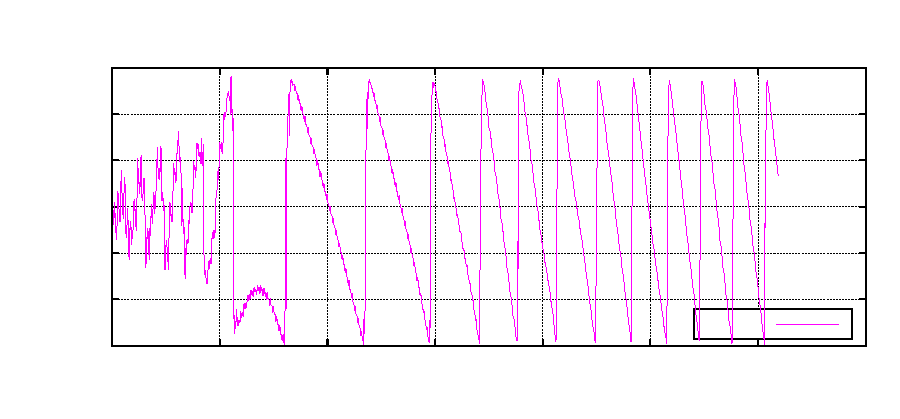
\includegraphics{diskperiastronh004q07}}%
    \gplfronttext
  \end{picture}%
\endgroup

	\end{center}
\end {figure}
\begin {figure}
	\begin{center}
		% GNUPLOT: LaTeX picture with Postscript
\begingroup
  \makeatletter
  \providecommand\color[2][]{%
    \GenericError{(gnuplot) \space\space\space\@spaces}{%
      Package color not loaded in conjunction with
      terminal option `colourtext'%
    }{See the gnuplot documentation for explanation.%
    }{Either use 'blacktext' in gnuplot or load the package
      color.sty in LaTeX.}%
    \renewcommand\color[2][]{}%
  }%
  \providecommand\includegraphics[2][]{%
    \GenericError{(gnuplot) \space\space\space\@spaces}{%
      Package graphicx or graphics not loaded%
    }{See the gnuplot documentation for explanation.%
    }{The gnuplot epslatex terminal needs graphicx.sty or graphics.sty.}%
    \renewcommand\includegraphics[2][]{}%
  }%
  \providecommand\rotatebox[2]{#2}%
  \@ifundefined{ifGPcolor}{%
    \newif\ifGPcolor
    \GPcolortrue
  }{}%
  \@ifundefined{ifGPblacktext}{%
    \newif\ifGPblacktext
    \GPblacktexttrue
  }{}%
  % define a \g@addto@macro without @ in the name:
  \let\gplgaddtomacro\g@addto@macro
  % define empty templates for all commands taking text:
  \gdef\gplbacktext{}%
  \gdef\gplfronttext{}%
  \makeatother
  \ifGPblacktext
    % no textcolor at all
    \def\colorrgb#1{}%
    \def\colorgray#1{}%
  \else
    % gray or color?
    \ifGPcolor
      \def\colorrgb#1{\color[rgb]{#1}}%
      \def\colorgray#1{\color[gray]{#1}}%
      \expandafter\def\csname LTw\endcsname{\color{white}}%
      \expandafter\def\csname LTb\endcsname{\color{black}}%
      \expandafter\def\csname LTa\endcsname{\color{black}}%
      \expandafter\def\csname LT0\endcsname{\color[rgb]{1,0,0}}%
      \expandafter\def\csname LT1\endcsname{\color[rgb]{0,1,0}}%
      \expandafter\def\csname LT2\endcsname{\color[rgb]{0,0,1}}%
      \expandafter\def\csname LT3\endcsname{\color[rgb]{1,0,1}}%
      \expandafter\def\csname LT4\endcsname{\color[rgb]{0,1,1}}%
      \expandafter\def\csname LT5\endcsname{\color[rgb]{1,1,0}}%
      \expandafter\def\csname LT6\endcsname{\color[rgb]{0,0,0}}%
      \expandafter\def\csname LT7\endcsname{\color[rgb]{1,0.3,0}}%
      \expandafter\def\csname LT8\endcsname{\color[rgb]{0.5,0.5,0.5}}%
    \else
      % gray
      \def\colorrgb#1{\color{black}}%
      \def\colorgray#1{\color[gray]{#1}}%
      \expandafter\def\csname LTw\endcsname{\color{white}}%
      \expandafter\def\csname LTb\endcsname{\color{black}}%
      \expandafter\def\csname LTa\endcsname{\color{black}}%
      \expandafter\def\csname LT0\endcsname{\color{black}}%
      \expandafter\def\csname LT1\endcsname{\color{black}}%
      \expandafter\def\csname LT2\endcsname{\color{black}}%
      \expandafter\def\csname LT3\endcsname{\color{black}}%
      \expandafter\def\csname LT4\endcsname{\color{black}}%
      \expandafter\def\csname LT5\endcsname{\color{black}}%
      \expandafter\def\csname LT6\endcsname{\color{black}}%
      \expandafter\def\csname LT7\endcsname{\color{black}}%
      \expandafter\def\csname LT8\endcsname{\color{black}}%
    \fi
  \fi
  \setlength{\unitlength}{0.0500bp}%
  \begin{picture}(8640.00,4032.00)%
    \gplgaddtomacro\gplbacktext{%
      \csname LTb\endcsname%
      \put(946,704){\makebox(0,0)[r]{\strut{}-4}}%
      \csname LTb\endcsname%
      \put(946,1085){\makebox(0,0)[r]{\strut{}-3}}%
      \csname LTb\endcsname%
      \put(946,1466){\makebox(0,0)[r]{\strut{}-2}}%
      \csname LTb\endcsname%
      \put(946,1847){\makebox(0,0)[r]{\strut{}-1}}%
      \csname LTb\endcsname%
      \put(946,2229){\makebox(0,0)[r]{\strut{} 0}}%
      \csname LTb\endcsname%
      \put(946,2610){\makebox(0,0)[r]{\strut{} 1}}%
      \csname LTb\endcsname%
      \put(946,2991){\makebox(0,0)[r]{\strut{} 2}}%
      \csname LTb\endcsname%
      \put(946,3372){\makebox(0,0)[r]{\strut{} 3}}%
      \csname LTb\endcsname%
      \put(1078,484){\makebox(0,0){\strut{} 0}}%
      \csname LTb\endcsname%
      \put(2283,484){\makebox(0,0){\strut{} 20}}%
      \csname LTb\endcsname%
      \put(3489,484){\makebox(0,0){\strut{} 40}}%
      \csname LTb\endcsname%
      \put(4694,484){\makebox(0,0){\strut{} 60}}%
      \csname LTb\endcsname%
      \put(5899,484){\makebox(0,0){\strut{} 80}}%
      \csname LTb\endcsname%
      \put(7105,484){\makebox(0,0){\strut{} 100}}%
      \csname LTb\endcsname%
      \put(8310,484){\makebox(0,0){\strut{} 120}}%
      \put(440,2038){\rotatebox{90}{\makebox(0,0){\strut{}Disk Periastron}}}%
      \put(4694,154){\makebox(0,0){\strut{}Time [$P_{\text{Orb}}$]}}%
      \put(4694,3702){\makebox(0,0){\strut{}h = 0.04}}%
    }%
    \gplgaddtomacro\gplfronttext{%
      \csname LTb\endcsname%
      \put(7323,910){\makebox(0,0)[r]{\strut{}q=0.8}}%
    }%
    \gplbacktext
    \put(0,0){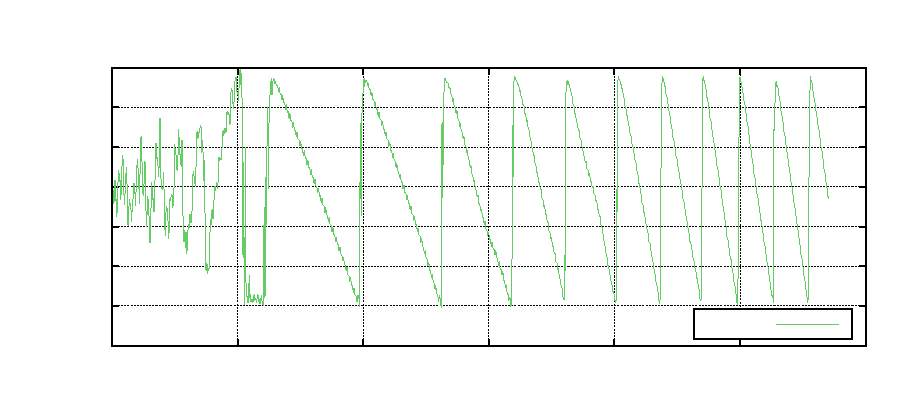
\includegraphics{diskperiastronh004q08}}%
    \gplfronttext
  \end{picture}%
\endgroup

	\end{center}
\end {figure}
\begin {figure}
	\begin{center}
		% GNUPLOT: LaTeX picture with Postscript
\begingroup
  \makeatletter
  \providecommand\color[2][]{%
    \GenericError{(gnuplot) \space\space\space\@spaces}{%
      Package color not loaded in conjunction with
      terminal option `colourtext'%
    }{See the gnuplot documentation for explanation.%
    }{Either use 'blacktext' in gnuplot or load the package
      color.sty in LaTeX.}%
    \renewcommand\color[2][]{}%
  }%
  \providecommand\includegraphics[2][]{%
    \GenericError{(gnuplot) \space\space\space\@spaces}{%
      Package graphicx or graphics not loaded%
    }{See the gnuplot documentation for explanation.%
    }{The gnuplot epslatex terminal needs graphicx.sty or graphics.sty.}%
    \renewcommand\includegraphics[2][]{}%
  }%
  \providecommand\rotatebox[2]{#2}%
  \@ifundefined{ifGPcolor}{%
    \newif\ifGPcolor
    \GPcolortrue
  }{}%
  \@ifundefined{ifGPblacktext}{%
    \newif\ifGPblacktext
    \GPblacktexttrue
  }{}%
  % define a \g@addto@macro without @ in the name:
  \let\gplgaddtomacro\g@addto@macro
  % define empty templates for all commands taking text:
  \gdef\gplbacktext{}%
  \gdef\gplfronttext{}%
  \makeatother
  \ifGPblacktext
    % no textcolor at all
    \def\colorrgb#1{}%
    \def\colorgray#1{}%
  \else
    % gray or color?
    \ifGPcolor
      \def\colorrgb#1{\color[rgb]{#1}}%
      \def\colorgray#1{\color[gray]{#1}}%
      \expandafter\def\csname LTw\endcsname{\color{white}}%
      \expandafter\def\csname LTb\endcsname{\color{black}}%
      \expandafter\def\csname LTa\endcsname{\color{black}}%
      \expandafter\def\csname LT0\endcsname{\color[rgb]{1,0,0}}%
      \expandafter\def\csname LT1\endcsname{\color[rgb]{0,1,0}}%
      \expandafter\def\csname LT2\endcsname{\color[rgb]{0,0,1}}%
      \expandafter\def\csname LT3\endcsname{\color[rgb]{1,0,1}}%
      \expandafter\def\csname LT4\endcsname{\color[rgb]{0,1,1}}%
      \expandafter\def\csname LT5\endcsname{\color[rgb]{1,1,0}}%
      \expandafter\def\csname LT6\endcsname{\color[rgb]{0,0,0}}%
      \expandafter\def\csname LT7\endcsname{\color[rgb]{1,0.3,0}}%
      \expandafter\def\csname LT8\endcsname{\color[rgb]{0.5,0.5,0.5}}%
    \else
      % gray
      \def\colorrgb#1{\color{black}}%
      \def\colorgray#1{\color[gray]{#1}}%
      \expandafter\def\csname LTw\endcsname{\color{white}}%
      \expandafter\def\csname LTb\endcsname{\color{black}}%
      \expandafter\def\csname LTa\endcsname{\color{black}}%
      \expandafter\def\csname LT0\endcsname{\color{black}}%
      \expandafter\def\csname LT1\endcsname{\color{black}}%
      \expandafter\def\csname LT2\endcsname{\color{black}}%
      \expandafter\def\csname LT3\endcsname{\color{black}}%
      \expandafter\def\csname LT4\endcsname{\color{black}}%
      \expandafter\def\csname LT5\endcsname{\color{black}}%
      \expandafter\def\csname LT6\endcsname{\color{black}}%
      \expandafter\def\csname LT7\endcsname{\color{black}}%
      \expandafter\def\csname LT8\endcsname{\color{black}}%
    \fi
  \fi
  \setlength{\unitlength}{0.0500bp}%
  \begin{picture}(8640.00,4032.00)%
    \gplgaddtomacro\gplbacktext{%
      \csname LTb\endcsname%
      \put(946,704){\makebox(0,0)[r]{\strut{}-4}}%
      \csname LTb\endcsname%
      \put(946,1085){\makebox(0,0)[r]{\strut{}-3}}%
      \csname LTb\endcsname%
      \put(946,1466){\makebox(0,0)[r]{\strut{}-2}}%
      \csname LTb\endcsname%
      \put(946,1847){\makebox(0,0)[r]{\strut{}-1}}%
      \csname LTb\endcsname%
      \put(946,2229){\makebox(0,0)[r]{\strut{} 0}}%
      \csname LTb\endcsname%
      \put(946,2610){\makebox(0,0)[r]{\strut{} 1}}%
      \csname LTb\endcsname%
      \put(946,2991){\makebox(0,0)[r]{\strut{} 2}}%
      \csname LTb\endcsname%
      \put(946,3372){\makebox(0,0)[r]{\strut{} 3}}%
      \csname LTb\endcsname%
      \put(1078,484){\makebox(0,0){\strut{} 0}}%
      \csname LTb\endcsname%
      \put(2283,484){\makebox(0,0){\strut{} 20}}%
      \csname LTb\endcsname%
      \put(3489,484){\makebox(0,0){\strut{} 40}}%
      \csname LTb\endcsname%
      \put(4694,484){\makebox(0,0){\strut{} 60}}%
      \csname LTb\endcsname%
      \put(5899,484){\makebox(0,0){\strut{} 80}}%
      \csname LTb\endcsname%
      \put(7105,484){\makebox(0,0){\strut{} 100}}%
      \csname LTb\endcsname%
      \put(8310,484){\makebox(0,0){\strut{} 120}}%
      \put(440,2038){\rotatebox{90}{\makebox(0,0){\strut{}Disk Periastron}}}%
      \put(4694,154){\makebox(0,0){\strut{}Time [$P_{\text{Orb}}$]}}%
      \put(4694,3702){\makebox(0,0){\strut{}h = 0.04}}%
    }%
    \gplgaddtomacro\gplfronttext{%
      \csname LTb\endcsname%
      \put(7323,910){\makebox(0,0)[r]{\strut{}q=0.9}}%
    }%
    \gplbacktext
    \put(0,0){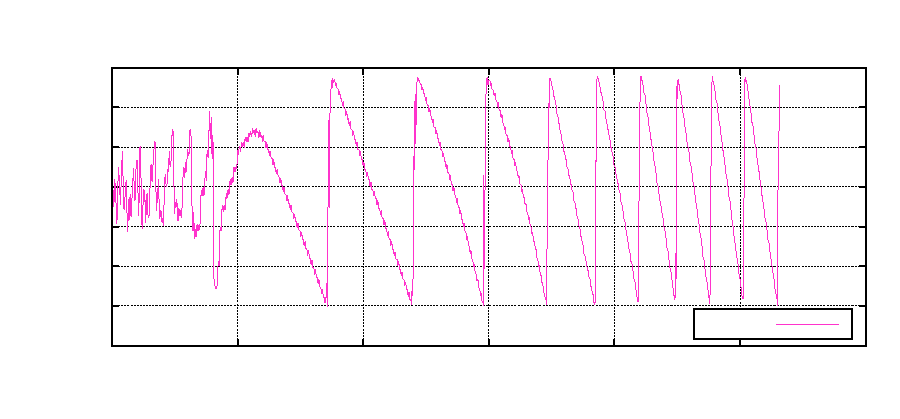
\includegraphics{diskperiastronh004q09}}%
    \gplfronttext
  \end{picture}%
\endgroup

	\end{center}
\end {figure}
\begin {figure}
	\begin{center}
		% GNUPLOT: LaTeX picture with Postscript
\begingroup
  \makeatletter
  \providecommand\color[2][]{%
    \GenericError{(gnuplot) \space\space\space\@spaces}{%
      Package color not loaded in conjunction with
      terminal option `colourtext'%
    }{See the gnuplot documentation for explanation.%
    }{Either use 'blacktext' in gnuplot or load the package
      color.sty in LaTeX.}%
    \renewcommand\color[2][]{}%
  }%
  \providecommand\includegraphics[2][]{%
    \GenericError{(gnuplot) \space\space\space\@spaces}{%
      Package graphicx or graphics not loaded%
    }{See the gnuplot documentation for explanation.%
    }{The gnuplot epslatex terminal needs graphicx.sty or graphics.sty.}%
    \renewcommand\includegraphics[2][]{}%
  }%
  \providecommand\rotatebox[2]{#2}%
  \@ifundefined{ifGPcolor}{%
    \newif\ifGPcolor
    \GPcolortrue
  }{}%
  \@ifundefined{ifGPblacktext}{%
    \newif\ifGPblacktext
    \GPblacktexttrue
  }{}%
  % define a \g@addto@macro without @ in the name:
  \let\gplgaddtomacro\g@addto@macro
  % define empty templates for all commands taking text:
  \gdef\gplbacktext{}%
  \gdef\gplfronttext{}%
  \makeatother
  \ifGPblacktext
    % no textcolor at all
    \def\colorrgb#1{}%
    \def\colorgray#1{}%
  \else
    % gray or color?
    \ifGPcolor
      \def\colorrgb#1{\color[rgb]{#1}}%
      \def\colorgray#1{\color[gray]{#1}}%
      \expandafter\def\csname LTw\endcsname{\color{white}}%
      \expandafter\def\csname LTb\endcsname{\color{black}}%
      \expandafter\def\csname LTa\endcsname{\color{black}}%
      \expandafter\def\csname LT0\endcsname{\color[rgb]{1,0,0}}%
      \expandafter\def\csname LT1\endcsname{\color[rgb]{0,1,0}}%
      \expandafter\def\csname LT2\endcsname{\color[rgb]{0,0,1}}%
      \expandafter\def\csname LT3\endcsname{\color[rgb]{1,0,1}}%
      \expandafter\def\csname LT4\endcsname{\color[rgb]{0,1,1}}%
      \expandafter\def\csname LT5\endcsname{\color[rgb]{1,1,0}}%
      \expandafter\def\csname LT6\endcsname{\color[rgb]{0,0,0}}%
      \expandafter\def\csname LT7\endcsname{\color[rgb]{1,0.3,0}}%
      \expandafter\def\csname LT8\endcsname{\color[rgb]{0.5,0.5,0.5}}%
    \else
      % gray
      \def\colorrgb#1{\color{black}}%
      \def\colorgray#1{\color[gray]{#1}}%
      \expandafter\def\csname LTw\endcsname{\color{white}}%
      \expandafter\def\csname LTb\endcsname{\color{black}}%
      \expandafter\def\csname LTa\endcsname{\color{black}}%
      \expandafter\def\csname LT0\endcsname{\color{black}}%
      \expandafter\def\csname LT1\endcsname{\color{black}}%
      \expandafter\def\csname LT2\endcsname{\color{black}}%
      \expandafter\def\csname LT3\endcsname{\color{black}}%
      \expandafter\def\csname LT4\endcsname{\color{black}}%
      \expandafter\def\csname LT5\endcsname{\color{black}}%
      \expandafter\def\csname LT6\endcsname{\color{black}}%
      \expandafter\def\csname LT7\endcsname{\color{black}}%
      \expandafter\def\csname LT8\endcsname{\color{black}}%
    \fi
  \fi
  \setlength{\unitlength}{0.0500bp}%
  \begin{picture}(8640.00,4032.00)%
    \gplgaddtomacro\gplbacktext{%
      \csname LTb\endcsname%
      \put(946,704){\makebox(0,0)[r]{\strut{}-4}}%
      \csname LTb\endcsname%
      \put(946,1085){\makebox(0,0)[r]{\strut{}-3}}%
      \csname LTb\endcsname%
      \put(946,1466){\makebox(0,0)[r]{\strut{}-2}}%
      \csname LTb\endcsname%
      \put(946,1847){\makebox(0,0)[r]{\strut{}-1}}%
      \csname LTb\endcsname%
      \put(946,2229){\makebox(0,0)[r]{\strut{} 0}}%
      \csname LTb\endcsname%
      \put(946,2610){\makebox(0,0)[r]{\strut{} 1}}%
      \csname LTb\endcsname%
      \put(946,2991){\makebox(0,0)[r]{\strut{} 2}}%
      \csname LTb\endcsname%
      \put(946,3372){\makebox(0,0)[r]{\strut{} 3}}%
      \csname LTb\endcsname%
      \put(1078,484){\makebox(0,0){\strut{} 0}}%
      \csname LTb\endcsname%
      \put(1801,484){\makebox(0,0){\strut{} 10}}%
      \csname LTb\endcsname%
      \put(2524,484){\makebox(0,0){\strut{} 20}}%
      \csname LTb\endcsname%
      \put(3248,484){\makebox(0,0){\strut{} 30}}%
      \csname LTb\endcsname%
      \put(3971,484){\makebox(0,0){\strut{} 40}}%
      \csname LTb\endcsname%
      \put(4694,484){\makebox(0,0){\strut{} 50}}%
      \csname LTb\endcsname%
      \put(5417,484){\makebox(0,0){\strut{} 60}}%
      \csname LTb\endcsname%
      \put(6140,484){\makebox(0,0){\strut{} 70}}%
      \csname LTb\endcsname%
      \put(6864,484){\makebox(0,0){\strut{} 80}}%
      \csname LTb\endcsname%
      \put(7587,484){\makebox(0,0){\strut{} 90}}%
      \csname LTb\endcsname%
      \put(8310,484){\makebox(0,0){\strut{} 100}}%
      \put(440,2038){\rotatebox{90}{\makebox(0,0){\strut{}Disk Periastron}}}%
      \put(4694,154){\makebox(0,0){\strut{}Time [$P_{\text{Orb}}$]}}%
      \put(4694,3702){\makebox(0,0){\strut{}h = 0.04}}%
    }%
    \gplgaddtomacro\gplfronttext{%
      \csname LTb\endcsname%
      \put(7323,910){\makebox(0,0)[r]{\strut{}q=1.0}}%
    }%
    \gplbacktext
    \put(0,0){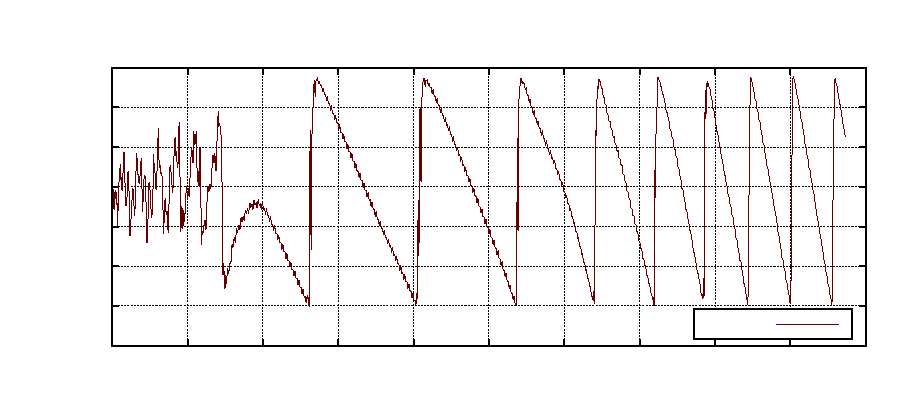
\includegraphics{diskperiastronh004q10}}%
    \gplfronttext
  \end{picture}%
\endgroup

	\end{center}
\end {figure}


\subsubsection{h = 0.03}
Bei einem h von 0.03 konnte nicht fuer alle MassRatios ein Gleichgewichtszustand der Exzentrizitaet erreicht werden. Ab einem Wert von q=0.5 sind die Disks nicht mehr exzentrisch, somit schwingt das Periastron um 0. Fuer kleinere Werte von q ist die Einschwingzeit recht lange, nur fuer q= 0.3 und q=0.4 sieht die Kurve gut aus.


sadfasdfafas
\begin {figure}
	\begin{center}
		% GNUPLOT: LaTeX picture with Postscript
\begingroup
  \makeatletter
  \providecommand\color[2][]{%
    \GenericError{(gnuplot) \space\space\space\@spaces}{%
      Package color not loaded in conjunction with
      terminal option `colourtext'%
    }{See the gnuplot documentation for explanation.%
    }{Either use 'blacktext' in gnuplot or load the package
      color.sty in LaTeX.}%
    \renewcommand\color[2][]{}%
  }%
  \providecommand\includegraphics[2][]{%
    \GenericError{(gnuplot) \space\space\space\@spaces}{%
      Package graphicx or graphics not loaded%
    }{See the gnuplot documentation for explanation.%
    }{The gnuplot epslatex terminal needs graphicx.sty or graphics.sty.}%
    \renewcommand\includegraphics[2][]{}%
  }%
  \providecommand\rotatebox[2]{#2}%
  \@ifundefined{ifGPcolor}{%
    \newif\ifGPcolor
    \GPcolortrue
  }{}%
  \@ifundefined{ifGPblacktext}{%
    \newif\ifGPblacktext
    \GPblacktexttrue
  }{}%
  % define a \g@addto@macro without @ in the name:
  \let\gplgaddtomacro\g@addto@macro
  % define empty templates for all commands taking text:
  \gdef\gplbacktext{}%
  \gdef\gplfronttext{}%
  \makeatother
  \ifGPblacktext
    % no textcolor at all
    \def\colorrgb#1{}%
    \def\colorgray#1{}%
  \else
    % gray or color?
    \ifGPcolor
      \def\colorrgb#1{\color[rgb]{#1}}%
      \def\colorgray#1{\color[gray]{#1}}%
      \expandafter\def\csname LTw\endcsname{\color{white}}%
      \expandafter\def\csname LTb\endcsname{\color{black}}%
      \expandafter\def\csname LTa\endcsname{\color{black}}%
      \expandafter\def\csname LT0\endcsname{\color[rgb]{1,0,0}}%
      \expandafter\def\csname LT1\endcsname{\color[rgb]{0,1,0}}%
      \expandafter\def\csname LT2\endcsname{\color[rgb]{0,0,1}}%
      \expandafter\def\csname LT3\endcsname{\color[rgb]{1,0,1}}%
      \expandafter\def\csname LT4\endcsname{\color[rgb]{0,1,1}}%
      \expandafter\def\csname LT5\endcsname{\color[rgb]{1,1,0}}%
      \expandafter\def\csname LT6\endcsname{\color[rgb]{0,0,0}}%
      \expandafter\def\csname LT7\endcsname{\color[rgb]{1,0.3,0}}%
      \expandafter\def\csname LT8\endcsname{\color[rgb]{0.5,0.5,0.5}}%
    \else
      % gray
      \def\colorrgb#1{\color{black}}%
      \def\colorgray#1{\color[gray]{#1}}%
      \expandafter\def\csname LTw\endcsname{\color{white}}%
      \expandafter\def\csname LTb\endcsname{\color{black}}%
      \expandafter\def\csname LTa\endcsname{\color{black}}%
      \expandafter\def\csname LT0\endcsname{\color{black}}%
      \expandafter\def\csname LT1\endcsname{\color{black}}%
      \expandafter\def\csname LT2\endcsname{\color{black}}%
      \expandafter\def\csname LT3\endcsname{\color{black}}%
      \expandafter\def\csname LT4\endcsname{\color{black}}%
      \expandafter\def\csname LT5\endcsname{\color{black}}%
      \expandafter\def\csname LT6\endcsname{\color{black}}%
      \expandafter\def\csname LT7\endcsname{\color{black}}%
      \expandafter\def\csname LT8\endcsname{\color{black}}%
    \fi
  \fi
  \setlength{\unitlength}{0.0500bp}%
  \begin{picture}(8640.00,4032.00)%
    \gplgaddtomacro\gplbacktext{%
      \csname LTb\endcsname%
      \put(946,704){\makebox(0,0)[r]{\strut{}-3}}%
      \csname LTb\endcsname%
      \put(946,1149){\makebox(0,0)[r]{\strut{}-2}}%
      \csname LTb\endcsname%
      \put(946,1593){\makebox(0,0)[r]{\strut{}-1}}%
      \csname LTb\endcsname%
      \put(946,2038){\makebox(0,0)[r]{\strut{} 0}}%
      \csname LTb\endcsname%
      \put(946,2483){\makebox(0,0)[r]{\strut{} 1}}%
      \csname LTb\endcsname%
      \put(946,2927){\makebox(0,0)[r]{\strut{} 2}}%
      \csname LTb\endcsname%
      \put(946,3372){\makebox(0,0)[r]{\strut{} 3}}%
      \csname LTb\endcsname%
      \put(1078,484){\makebox(0,0){\strut{} 0}}%
      \csname LTb\endcsname%
      \put(1982,484){\makebox(0,0){\strut{} 20}}%
      \csname LTb\endcsname%
      \put(2886,484){\makebox(0,0){\strut{} 40}}%
      \csname LTb\endcsname%
      \put(3790,484){\makebox(0,0){\strut{} 60}}%
      \csname LTb\endcsname%
      \put(4694,484){\makebox(0,0){\strut{} 80}}%
      \csname LTb\endcsname%
      \put(5598,484){\makebox(0,0){\strut{} 100}}%
      \csname LTb\endcsname%
      \put(6502,484){\makebox(0,0){\strut{} 120}}%
      \csname LTb\endcsname%
      \put(7406,484){\makebox(0,0){\strut{} 140}}%
      \csname LTb\endcsname%
      \put(8310,484){\makebox(0,0){\strut{} 160}}%
      \put(440,2038){\rotatebox{90}{\makebox(0,0){\strut{}Disk Periastron}}}%
      \put(4694,154){\makebox(0,0){\strut{}Time [$P_{\text{Orb}}$]}}%
      \put(4694,3702){\makebox(0,0){\strut{}h = 0.03}}%
    }%
    \gplgaddtomacro\gplfronttext{%
      \csname LTb\endcsname%
      \put(7323,910){\makebox(0,0)[r]{\strut{}q=0.1}}%
    }%
    \gplbacktext
    \put(0,0){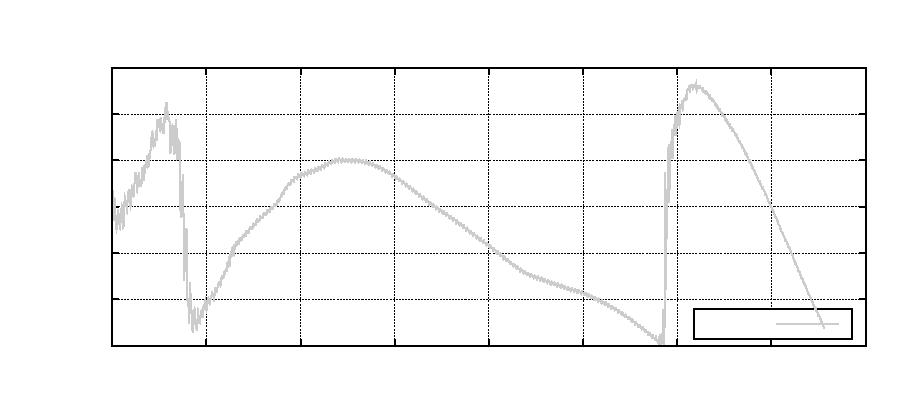
\includegraphics{diskperiastronh003q01}}%
    \gplfronttext
  \end{picture}%
\endgroup

	\end{center}
\end {figure}
\begin {figure}
	\begin{center}
		% GNUPLOT: LaTeX picture with Postscript
\begingroup
  \makeatletter
  \providecommand\color[2][]{%
    \GenericError{(gnuplot) \space\space\space\@spaces}{%
      Package color not loaded in conjunction with
      terminal option `colourtext'%
    }{See the gnuplot documentation for explanation.%
    }{Either use 'blacktext' in gnuplot or load the package
      color.sty in LaTeX.}%
    \renewcommand\color[2][]{}%
  }%
  \providecommand\includegraphics[2][]{%
    \GenericError{(gnuplot) \space\space\space\@spaces}{%
      Package graphicx or graphics not loaded%
    }{See the gnuplot documentation for explanation.%
    }{The gnuplot epslatex terminal needs graphicx.sty or graphics.sty.}%
    \renewcommand\includegraphics[2][]{}%
  }%
  \providecommand\rotatebox[2]{#2}%
  \@ifundefined{ifGPcolor}{%
    \newif\ifGPcolor
    \GPcolortrue
  }{}%
  \@ifundefined{ifGPblacktext}{%
    \newif\ifGPblacktext
    \GPblacktexttrue
  }{}%
  % define a \g@addto@macro without @ in the name:
  \let\gplgaddtomacro\g@addto@macro
  % define empty templates for all commands taking text:
  \gdef\gplbacktext{}%
  \gdef\gplfronttext{}%
  \makeatother
  \ifGPblacktext
    % no textcolor at all
    \def\colorrgb#1{}%
    \def\colorgray#1{}%
  \else
    % gray or color?
    \ifGPcolor
      \def\colorrgb#1{\color[rgb]{#1}}%
      \def\colorgray#1{\color[gray]{#1}}%
      \expandafter\def\csname LTw\endcsname{\color{white}}%
      \expandafter\def\csname LTb\endcsname{\color{black}}%
      \expandafter\def\csname LTa\endcsname{\color{black}}%
      \expandafter\def\csname LT0\endcsname{\color[rgb]{1,0,0}}%
      \expandafter\def\csname LT1\endcsname{\color[rgb]{0,1,0}}%
      \expandafter\def\csname LT2\endcsname{\color[rgb]{0,0,1}}%
      \expandafter\def\csname LT3\endcsname{\color[rgb]{1,0,1}}%
      \expandafter\def\csname LT4\endcsname{\color[rgb]{0,1,1}}%
      \expandafter\def\csname LT5\endcsname{\color[rgb]{1,1,0}}%
      \expandafter\def\csname LT6\endcsname{\color[rgb]{0,0,0}}%
      \expandafter\def\csname LT7\endcsname{\color[rgb]{1,0.3,0}}%
      \expandafter\def\csname LT8\endcsname{\color[rgb]{0.5,0.5,0.5}}%
    \else
      % gray
      \def\colorrgb#1{\color{black}}%
      \def\colorgray#1{\color[gray]{#1}}%
      \expandafter\def\csname LTw\endcsname{\color{white}}%
      \expandafter\def\csname LTb\endcsname{\color{black}}%
      \expandafter\def\csname LTa\endcsname{\color{black}}%
      \expandafter\def\csname LT0\endcsname{\color{black}}%
      \expandafter\def\csname LT1\endcsname{\color{black}}%
      \expandafter\def\csname LT2\endcsname{\color{black}}%
      \expandafter\def\csname LT3\endcsname{\color{black}}%
      \expandafter\def\csname LT4\endcsname{\color{black}}%
      \expandafter\def\csname LT5\endcsname{\color{black}}%
      \expandafter\def\csname LT6\endcsname{\color{black}}%
      \expandafter\def\csname LT7\endcsname{\color{black}}%
      \expandafter\def\csname LT8\endcsname{\color{black}}%
    \fi
  \fi
  \setlength{\unitlength}{0.0500bp}%
  \begin{picture}(8640.00,4032.00)%
    \gplgaddtomacro\gplbacktext{%
      \csname LTb\endcsname%
      \put(946,704){\makebox(0,0)[r]{\strut{}-4}}%
      \csname LTb\endcsname%
      \put(946,1085){\makebox(0,0)[r]{\strut{}-3}}%
      \csname LTb\endcsname%
      \put(946,1466){\makebox(0,0)[r]{\strut{}-2}}%
      \csname LTb\endcsname%
      \put(946,1847){\makebox(0,0)[r]{\strut{}-1}}%
      \csname LTb\endcsname%
      \put(946,2229){\makebox(0,0)[r]{\strut{} 0}}%
      \csname LTb\endcsname%
      \put(946,2610){\makebox(0,0)[r]{\strut{} 1}}%
      \csname LTb\endcsname%
      \put(946,2991){\makebox(0,0)[r]{\strut{} 2}}%
      \csname LTb\endcsname%
      \put(946,3372){\makebox(0,0)[r]{\strut{} 3}}%
      \csname LTb\endcsname%
      \put(1078,484){\makebox(0,0){\strut{} 0}}%
      \csname LTb\endcsname%
      \put(1982,484){\makebox(0,0){\strut{} 20}}%
      \csname LTb\endcsname%
      \put(2886,484){\makebox(0,0){\strut{} 40}}%
      \csname LTb\endcsname%
      \put(3790,484){\makebox(0,0){\strut{} 60}}%
      \csname LTb\endcsname%
      \put(4694,484){\makebox(0,0){\strut{} 80}}%
      \csname LTb\endcsname%
      \put(5598,484){\makebox(0,0){\strut{} 100}}%
      \csname LTb\endcsname%
      \put(6502,484){\makebox(0,0){\strut{} 120}}%
      \csname LTb\endcsname%
      \put(7406,484){\makebox(0,0){\strut{} 140}}%
      \csname LTb\endcsname%
      \put(8310,484){\makebox(0,0){\strut{} 160}}%
      \put(440,2038){\rotatebox{90}{\makebox(0,0){\strut{}Disk Periastron}}}%
      \put(4694,154){\makebox(0,0){\strut{}Time [$P_{\text{Orb}}$]}}%
      \put(4694,3702){\makebox(0,0){\strut{}h = 0.03}}%
    }%
    \gplgaddtomacro\gplfronttext{%
      \csname LTb\endcsname%
      \put(7323,910){\makebox(0,0)[r]{\strut{}q=0.2}}%
    }%
    \gplbacktext
    \put(0,0){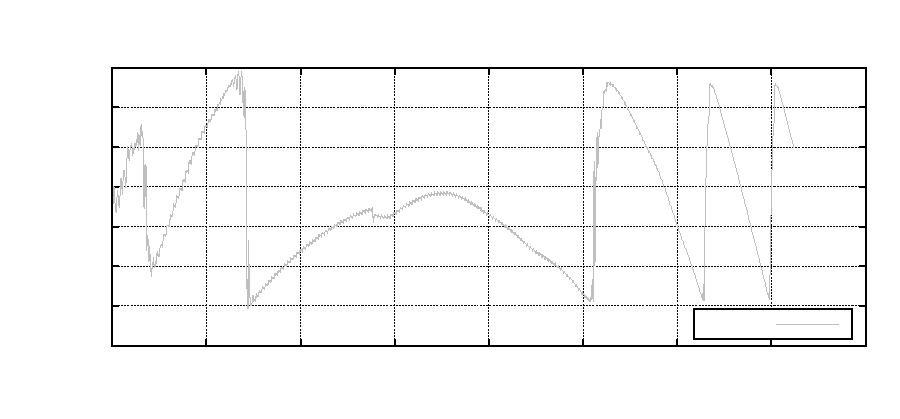
\includegraphics{diskperiastronh003q02}}%
    \gplfronttext
  \end{picture}%
\endgroup

	\end{center}
\end {figure}

\begin {figure}
	\begin{center}
		% GNUPLOT: LaTeX picture with Postscript
\begingroup
  \makeatletter
  \providecommand\color[2][]{%
    \GenericError{(gnuplot) \space\space\space\@spaces}{%
      Package color not loaded in conjunction with
      terminal option `colourtext'%
    }{See the gnuplot documentation for explanation.%
    }{Either use 'blacktext' in gnuplot or load the package
      color.sty in LaTeX.}%
    \renewcommand\color[2][]{}%
  }%
  \providecommand\includegraphics[2][]{%
    \GenericError{(gnuplot) \space\space\space\@spaces}{%
      Package graphicx or graphics not loaded%
    }{See the gnuplot documentation for explanation.%
    }{The gnuplot epslatex terminal needs graphicx.sty or graphics.sty.}%
    \renewcommand\includegraphics[2][]{}%
  }%
  \providecommand\rotatebox[2]{#2}%
  \@ifundefined{ifGPcolor}{%
    \newif\ifGPcolor
    \GPcolortrue
  }{}%
  \@ifundefined{ifGPblacktext}{%
    \newif\ifGPblacktext
    \GPblacktexttrue
  }{}%
  % define a \g@addto@macro without @ in the name:
  \let\gplgaddtomacro\g@addto@macro
  % define empty templates for all commands taking text:
  \gdef\gplbacktext{}%
  \gdef\gplfronttext{}%
  \makeatother
  \ifGPblacktext
    % no textcolor at all
    \def\colorrgb#1{}%
    \def\colorgray#1{}%
  \else
    % gray or color?
    \ifGPcolor
      \def\colorrgb#1{\color[rgb]{#1}}%
      \def\colorgray#1{\color[gray]{#1}}%
      \expandafter\def\csname LTw\endcsname{\color{white}}%
      \expandafter\def\csname LTb\endcsname{\color{black}}%
      \expandafter\def\csname LTa\endcsname{\color{black}}%
      \expandafter\def\csname LT0\endcsname{\color[rgb]{1,0,0}}%
      \expandafter\def\csname LT1\endcsname{\color[rgb]{0,1,0}}%
      \expandafter\def\csname LT2\endcsname{\color[rgb]{0,0,1}}%
      \expandafter\def\csname LT3\endcsname{\color[rgb]{1,0,1}}%
      \expandafter\def\csname LT4\endcsname{\color[rgb]{0,1,1}}%
      \expandafter\def\csname LT5\endcsname{\color[rgb]{1,1,0}}%
      \expandafter\def\csname LT6\endcsname{\color[rgb]{0,0,0}}%
      \expandafter\def\csname LT7\endcsname{\color[rgb]{1,0.3,0}}%
      \expandafter\def\csname LT8\endcsname{\color[rgb]{0.5,0.5,0.5}}%
    \else
      % gray
      \def\colorrgb#1{\color{black}}%
      \def\colorgray#1{\color[gray]{#1}}%
      \expandafter\def\csname LTw\endcsname{\color{white}}%
      \expandafter\def\csname LTb\endcsname{\color{black}}%
      \expandafter\def\csname LTa\endcsname{\color{black}}%
      \expandafter\def\csname LT0\endcsname{\color{black}}%
      \expandafter\def\csname LT1\endcsname{\color{black}}%
      \expandafter\def\csname LT2\endcsname{\color{black}}%
      \expandafter\def\csname LT3\endcsname{\color{black}}%
      \expandafter\def\csname LT4\endcsname{\color{black}}%
      \expandafter\def\csname LT5\endcsname{\color{black}}%
      \expandafter\def\csname LT6\endcsname{\color{black}}%
      \expandafter\def\csname LT7\endcsname{\color{black}}%
      \expandafter\def\csname LT8\endcsname{\color{black}}%
    \fi
  \fi
  \setlength{\unitlength}{0.0500bp}%
  \begin{picture}(8640.00,4032.00)%
    \gplgaddtomacro\gplbacktext{%
      \csname LTb\endcsname%
      \put(1210,704){\makebox(0,0)[r]{\strut{}-1.5}}%
      \csname LTb\endcsname%
      \put(1210,1149){\makebox(0,0)[r]{\strut{}-1}}%
      \csname LTb\endcsname%
      \put(1210,1593){\makebox(0,0)[r]{\strut{}-0.5}}%
      \csname LTb\endcsname%
      \put(1210,2038){\makebox(0,0)[r]{\strut{} 0}}%
      \csname LTb\endcsname%
      \put(1210,2483){\makebox(0,0)[r]{\strut{} 0.5}}%
      \csname LTb\endcsname%
      \put(1210,2927){\makebox(0,0)[r]{\strut{} 1}}%
      \csname LTb\endcsname%
      \put(1210,3372){\makebox(0,0)[r]{\strut{} 1.5}}%
      \csname LTb\endcsname%
      \put(1342,484){\makebox(0,0){\strut{} 0}}%
      \csname LTb\endcsname%
      \put(2503,484){\makebox(0,0){\strut{} 20}}%
      \csname LTb\endcsname%
      \put(3665,484){\makebox(0,0){\strut{} 40}}%
      \csname LTb\endcsname%
      \put(4826,484){\makebox(0,0){\strut{} 60}}%
      \csname LTb\endcsname%
      \put(5987,484){\makebox(0,0){\strut{} 80}}%
      \csname LTb\endcsname%
      \put(7149,484){\makebox(0,0){\strut{} 100}}%
      \csname LTb\endcsname%
      \put(8310,484){\makebox(0,0){\strut{} 120}}%
      \put(440,2038){\rotatebox{90}{\makebox(0,0){\strut{}Disk Periastron}}}%
      \put(4826,154){\makebox(0,0){\strut{}Time [$P_{\text{Orb}}$]}}%
      \put(4826,3702){\makebox(0,0){\strut{}h = 0.03}}%
    }%
    \gplgaddtomacro\gplfronttext{%
      \csname LTb\endcsname%
      \put(7323,910){\makebox(0,0)[r]{\strut{}q=0.9}}%
    }%
    \gplbacktext
    \put(0,0){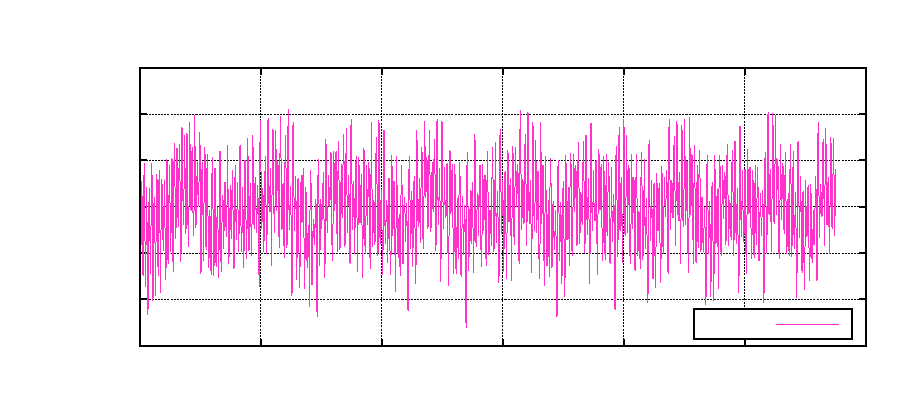
\includegraphics{diskperiastronh003q09}}%
    \gplfronttext
  \end{picture}%
\endgroup

	\end{center}
\end {figure}
\begin {figure}
	\begin{center}
		% GNUPLOT: LaTeX picture with Postscript
\begingroup
  \makeatletter
  \providecommand\color[2][]{%
    \GenericError{(gnuplot) \space\space\space\@spaces}{%
      Package color not loaded in conjunction with
      terminal option `colourtext'%
    }{See the gnuplot documentation for explanation.%
    }{Either use 'blacktext' in gnuplot or load the package
      color.sty in LaTeX.}%
    \renewcommand\color[2][]{}%
  }%
  \providecommand\includegraphics[2][]{%
    \GenericError{(gnuplot) \space\space\space\@spaces}{%
      Package graphicx or graphics not loaded%
    }{See the gnuplot documentation for explanation.%
    }{The gnuplot epslatex terminal needs graphicx.sty or graphics.sty.}%
    \renewcommand\includegraphics[2][]{}%
  }%
  \providecommand\rotatebox[2]{#2}%
  \@ifundefined{ifGPcolor}{%
    \newif\ifGPcolor
    \GPcolortrue
  }{}%
  \@ifundefined{ifGPblacktext}{%
    \newif\ifGPblacktext
    \GPblacktexttrue
  }{}%
  % define a \g@addto@macro without @ in the name:
  \let\gplgaddtomacro\g@addto@macro
  % define empty templates for all commands taking text:
  \gdef\gplbacktext{}%
  \gdef\gplfronttext{}%
  \makeatother
  \ifGPblacktext
    % no textcolor at all
    \def\colorrgb#1{}%
    \def\colorgray#1{}%
  \else
    % gray or color?
    \ifGPcolor
      \def\colorrgb#1{\color[rgb]{#1}}%
      \def\colorgray#1{\color[gray]{#1}}%
      \expandafter\def\csname LTw\endcsname{\color{white}}%
      \expandafter\def\csname LTb\endcsname{\color{black}}%
      \expandafter\def\csname LTa\endcsname{\color{black}}%
      \expandafter\def\csname LT0\endcsname{\color[rgb]{1,0,0}}%
      \expandafter\def\csname LT1\endcsname{\color[rgb]{0,1,0}}%
      \expandafter\def\csname LT2\endcsname{\color[rgb]{0,0,1}}%
      \expandafter\def\csname LT3\endcsname{\color[rgb]{1,0,1}}%
      \expandafter\def\csname LT4\endcsname{\color[rgb]{0,1,1}}%
      \expandafter\def\csname LT5\endcsname{\color[rgb]{1,1,0}}%
      \expandafter\def\csname LT6\endcsname{\color[rgb]{0,0,0}}%
      \expandafter\def\csname LT7\endcsname{\color[rgb]{1,0.3,0}}%
      \expandafter\def\csname LT8\endcsname{\color[rgb]{0.5,0.5,0.5}}%
    \else
      % gray
      \def\colorrgb#1{\color{black}}%
      \def\colorgray#1{\color[gray]{#1}}%
      \expandafter\def\csname LTw\endcsname{\color{white}}%
      \expandafter\def\csname LTb\endcsname{\color{black}}%
      \expandafter\def\csname LTa\endcsname{\color{black}}%
      \expandafter\def\csname LT0\endcsname{\color{black}}%
      \expandafter\def\csname LT1\endcsname{\color{black}}%
      \expandafter\def\csname LT2\endcsname{\color{black}}%
      \expandafter\def\csname LT3\endcsname{\color{black}}%
      \expandafter\def\csname LT4\endcsname{\color{black}}%
      \expandafter\def\csname LT5\endcsname{\color{black}}%
      \expandafter\def\csname LT6\endcsname{\color{black}}%
      \expandafter\def\csname LT7\endcsname{\color{black}}%
      \expandafter\def\csname LT8\endcsname{\color{black}}%
    \fi
  \fi
  \setlength{\unitlength}{0.0500bp}%
  \begin{picture}(8640.00,4032.00)%
    \gplgaddtomacro\gplbacktext{%
      \csname LTb\endcsname%
      \put(1210,704){\makebox(0,0)[r]{\strut{}-1.5}}%
      \csname LTb\endcsname%
      \put(1210,1149){\makebox(0,0)[r]{\strut{}-1}}%
      \csname LTb\endcsname%
      \put(1210,1593){\makebox(0,0)[r]{\strut{}-0.5}}%
      \csname LTb\endcsname%
      \put(1210,2038){\makebox(0,0)[r]{\strut{} 0}}%
      \csname LTb\endcsname%
      \put(1210,2483){\makebox(0,0)[r]{\strut{} 0.5}}%
      \csname LTb\endcsname%
      \put(1210,2927){\makebox(0,0)[r]{\strut{} 1}}%
      \csname LTb\endcsname%
      \put(1210,3372){\makebox(0,0)[r]{\strut{} 1.5}}%
      \csname LTb\endcsname%
      \put(1342,484){\makebox(0,0){\strut{} 0}}%
      \csname LTb\endcsname%
      \put(2503,484){\makebox(0,0){\strut{} 20}}%
      \csname LTb\endcsname%
      \put(3665,484){\makebox(0,0){\strut{} 40}}%
      \csname LTb\endcsname%
      \put(4826,484){\makebox(0,0){\strut{} 60}}%
      \csname LTb\endcsname%
      \put(5987,484){\makebox(0,0){\strut{} 80}}%
      \csname LTb\endcsname%
      \put(7149,484){\makebox(0,0){\strut{} 100}}%
      \csname LTb\endcsname%
      \put(8310,484){\makebox(0,0){\strut{} 120}}%
      \put(440,2038){\rotatebox{90}{\makebox(0,0){\strut{}Disk Periastron}}}%
      \put(4826,154){\makebox(0,0){\strut{}Time [$P_{\text{Orb}}$]}}%
      \put(4826,3702){\makebox(0,0){\strut{}h = 0.03}}%
    }%
    \gplgaddtomacro\gplfronttext{%
      \csname LTb\endcsname%
      \put(7323,910){\makebox(0,0)[r]{\strut{}q=1.0}}%
    }%
    \gplbacktext
    \put(0,0){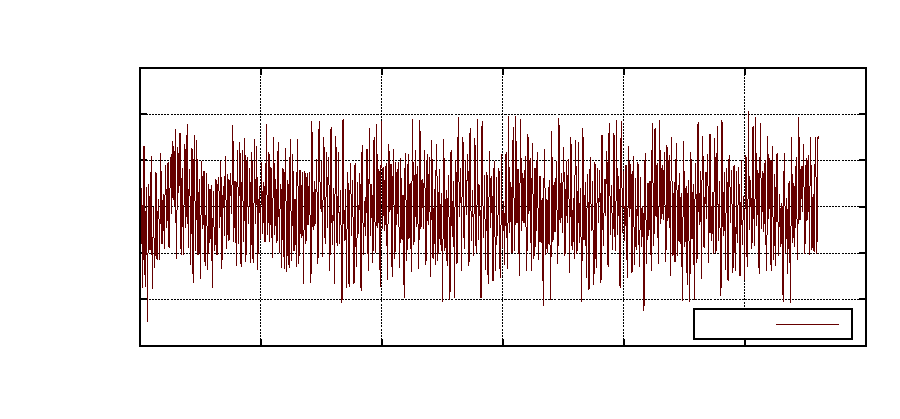
\includegraphics{diskperiastronh003q10}}%
    \gplfronttext
  \end{picture}%
\endgroup

	\end{center}
\end {figure}

\end{document}

